\documentclass{article}
% Commands
\newcommand{\ASSNMT}{Project Necromancer}
\newcommand{\CLASS}{Design Document}
\newcommand{\Footer}{Grand Valley State University}

\newcommand{\DATE}{July 2015}

% Packages
\usepackage[utf8]{inputenc}
\usepackage[T1]{fontenc}
\usepackage{lmodern}
\usepackage{pdflscape}
\usepackage{geometry}
\usepackage[usenames,dvipsnames]{xcolor}
\usepackage{graphicx}
\usepackage{mathtools}
\usepackage[justification=centering]{caption}
\usepackage{amssymb}
\usepackage[pdftex, pdfborderstyle={/S/U/W 0}]{hyperref} % this disables the boxes around links]
\usepackage{float}
\usepackage{listings}
% \usepackage{color}
\usepackage{enumitem}
\usepackage{fancyhdr}
\usepackage{caption}
\numberwithin{figure}{section}
\usepackage{amsmath}


\numberwithin{equation}{section}
% lstlisting
\definecolor{dkgreen}{rgb}{0,0.6,0}
\definecolor{gray}{rgb}{0.5,0.5,0.5}
\definecolor{mauve}{rgb}{0.58,0,0.82}
\lstset
{
  frame=single,
  frameround=tttt,
  language=C,
  numberstyle=\tiny\color{gray},
  keywordstyle=\color{blue},
  commentstyle=\color{dkgreen},
  stringstyle=\color{mauve},
  tabsize=3,
  breaklines=true,
  basicstyle={\small\ttfamily},
  xleftmargin=\fboxsep,
  xrightmargin=-\fboxsep,
  numbers = left,
  stepnumber = 5,
  firstnumber = 1
}

% macro for appendix to be printed as "Appendix A {name of appendix}"
% instead of "A {name of appendix}"
% From: http://tex.stackexchange.com/questions/160839/having-appendix-a-instead-of-a-appendix
\makeatletter
%% The "\@seccntformat" command is an auxiliary command
%% (see pp. 26f. of 'The LaTeX Companion,' 2nd. ed.)
\def\@seccntformat#1{\@ifundefined{#1@cntformat}%
   {\csname the#1\endcsname\quad}  % default
   {\csname #1@cntformat\endcsname}% enable individual control
}
\let\oldappendix\appendix %% save current definition of \appendix
\renewcommand\appendix{%
    \oldappendix
    \newcommand{\section@cntformat}{\appendixname~\thesection\quad}
}
\makeatother
% Sign and Date command
\newcommand{\namesigdate}[2][5cm]{%
  \begin{tabular}{@{}p{#1}@{}}
    #2 \\[2\normalbaselineskip] \hrule \\[0pt]
    {\small \textit{Signature}} \\[2\normalbaselineskip] \hrule \\[0pt]
    {\small \textit{Date}}
  \end{tabular}
}


\begin{document}
% =====----- Initial Set Up -----=====
% Title Page
\newgeometry{top=2cm,left=1cm,bottom=1cm,right=1cm}
\begin{flushleft}
\pagenumbering{gobble}

\textsc{\LARGE \bfseries \ASSNMT}\\

\textsc{\Large \CLASS}\\[0.2cm]
\linethickness{0.5mm}
{\color{ForestGreen}\line(1,0){350}} \\ [1.0cm]

\begin{flushleft} \large
\begin{tabular}{lll}
  Sponsored By: & The Rainforest Connection (RFCx) 
\includegraphics[height=0.4cm]{rfcxlogo} & \\
                &               & \\
  Submitted By: & Joe Gibson    & \href{mailto:gibsjose@mail.gvsu.edu}{gibsjose@mail.gvsu.edu}\\
              & David Adlof     & \href{mailto:adlofd@mail.gvsu.edu}{adlofd@mail.gvsu.edu}\\
              & Kalee Stutzman  & \href{mailto:stutzmak@mail.gvsu.edu}{stutzmak@mail.gvsu.edu}\\
              & Jesse Millwood  & \href{mailto:millwooj@mail.gvsu.edu}{millwooj@mail.gvsu.edu}\\
\end{tabular}

\bigskip

\bigskip
Date Submitted: \DATE
\end{flushleft}

\smallskip
{\color{ForestGreen}\line(1,0){350}} \\ [1.0cm]
\section*{Executive Summary} \label{sect:execsum}
Software, electrical, and hardware enhancements to Rainforest Connection’s currently used device are proposed in this paper. The electrical enhancements include the addition of a new PCB that contains power regulation and battery charging circuitry, along with current, voltage, temperature, and humidity sensors. The software enhancements include sending sensor measurements to an Android cellphone. Sending measurements from the PCB to the phone will allow for diagnostic feedback that can be used for laboratory testing and verification as well as field statistics. The point of this project is not to entirely redesign the existing device but rather to provide modular enhancements and improvements to specific components.

\bigskip
Power consumption is a major concern and a key area for improvement on the existing device. We will use \textit{Max Point Power Tracking}(MPPT) ICs in the design of the power regulation and solar panel interface to ensure maximum efficiency from the solar panels. In addition we will use Lithium-Ion battery management ICs to ensure that the batteries are properly charged, properly discharged, and to prevent overheating. A switching power regulator will boost the voltage from either the batteries or the solar panel to charge the phone and a linear dropout regulator will provide 3.3V to the regulation and diagnostic circuitry on the PCB.

\bigskip
Temperature is another major concern. To mitigate the heat produced by the phone, the power circuitry, and the environment, a heatsink will be attached to the PCB with direct thermal contact with the phone. The heatsink will extend outside of the enclosure, transferring heat outside of the device enclosure.

\bigskip
Sending diagnostics will be achieved using an 8-bit Atmel ATmega328P microcontroller. Power, temperature, and humidity data will be sent from the microcontroller to the cell phone via USB, where it will be received and displayed by an Android application.

\section*{Keywords} \label{sect:keywords}
Rain forest, Recycling, RFCx, Rainforest Connection, cellphone, Android, logging

\vfill

% Bottom of the page
\begin{center}
{\large \Footer}
\end{center}
\begin{figure}[H]
  \centering
  
\includegraphics[width=.1\textwidth]{small_gvsu}
\end{figure}
\end{flushleft}
\restoregeometry
\newpage
% Define Page Geometry for rest of report
{\newgeometry{left=0.8in, right=0.8in, top=1in, bottom=1in}
% Page Numbers
\pagenumbering{arabic}
\pagestyle{fancy}
\fancyhf{}
\lhead{\ASSNMT}
\rhead{\leftmark}
\rfoot{Page \thepage}
% No paragraph indents
\setlength{\parindent}{0cm}
% =====----- Rest of Report -----=====
\newpage
\tableofcontents
\newpage
%%%%%%%%%%%%%%%%%%%%%%%%%%%%%%%%%%%%%%%%%%%%%%%%%%%%%%%%%% BACKGROUND %%%%%%%%%%%%%%%%%%%%%%%%%%%%%%%%%%%%%%%%%%%%%%%%%%%%%%%%%%
\section{RFCx Background} \label{sect:background}
Rainforest Connection (RFCx) is a non-profit organization that is dedicated to stopping illegal logging and deforestation in rainforests throughout the world. The destruction of tropical rainforests is a leading cause of carbon dioxide emission, and much of it is caused by illegal activities. RFCx combats illegal logging with devices using re-purposed cell-phones strategically placed in trees in remote areas. A picture of the entire device is shown below in Figure \ref{fig:device}.

\begin{figure}[H]
  \centering
  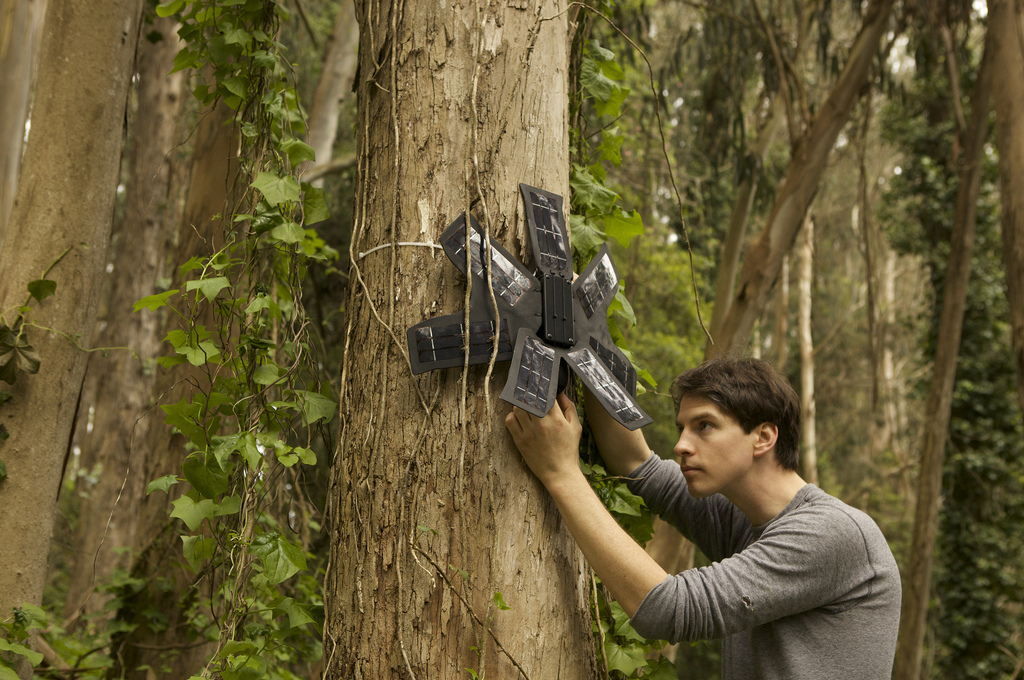
\includegraphics[width=0.8\textwidth]{device}
  \caption{RFCx President Topher White installing an existing device in the rainforests of Borneo}
  \label{fig:device}
\end{figure}
\newpage

These devices record and analyze audio, using their data connection to periodically send audio data to the RFCx server. Digital signal processing algorithms are used to detect the sound of chainsaws and engines at a distance of up to $\frac{2}{3}$ of a mile. If a chainsaw is detected, an alert is sent to pre-existing ground patrols, who can react to the situation and combat the threat. In addition to man-made sounds, the RFCx platform is also used to record the sounds of animals in the forest. These sounds can be used to gain information about certain species of animals and are open to anyone to use and analyze. Because of the sheer size of the area, it is impractical, if not impossible, for foot patrols to properly monitor the forests for illegal activities without the aid of technology. The flow of data, from audio collection to human intervention, is shown below in Figure \ref{fig:infographic}.

\begin{figure}[H]
  \centering
  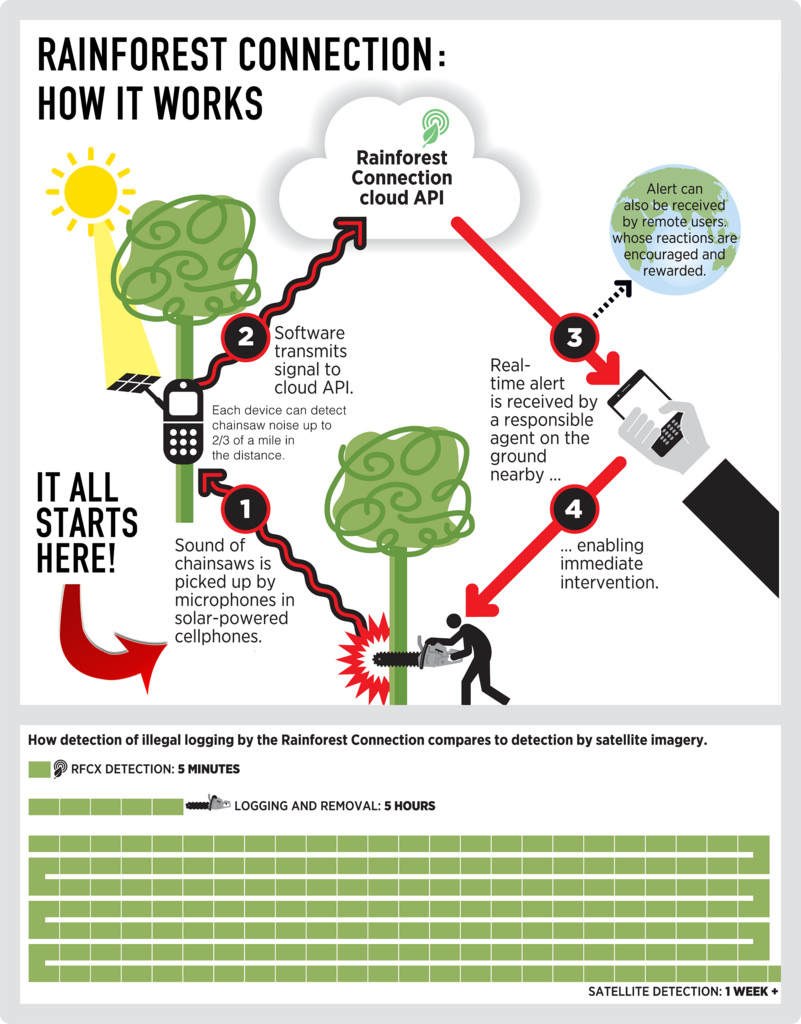
\includegraphics[height=0.76\textwidth]{infographic}
  \caption{Infographic from RFCx website (\href{www.rfcx.org}{www.rfcx.org}) showing the flow of data}
  \label{fig:infographic}
\end{figure}
\newpage

%%%%%%%%%%%%%%%%%%%%%%%%%%%%%%%%%%%%%%%%%%%%%%%%%%%%%%%%% INTRODUCTION %%%%%%%%%%%%%%%%%%%%%%%%%%%%%%%%%%%%%%%%%%%%%%%%%%%%%%%%%
\section{Project Introduction} \label{sect:intro}
RFCx Project Necromancer is primarily comprised of enhancements to the existing system in the areas of power consumption, power efficiency, temperature concerns, and overall modularity of components. The devices currently consist of an Android phone, Radioshack enclosure, off-the-shelf external microhpone and antenna, RFCx solar petals, two dual-cell Lithium-Ion batteries, and  various off-the-shelf PCBs and individual electrical components comprising the power regulation and solar and battery management control. The external microphone, antenna, solar petals, batteries (Appendix \ref{fig:batdat}), and Android phone will remain the same. A view inside of the device is shown in Figure \ref{fig:device_inside}.

\begin{figure}[H]
  \centering
  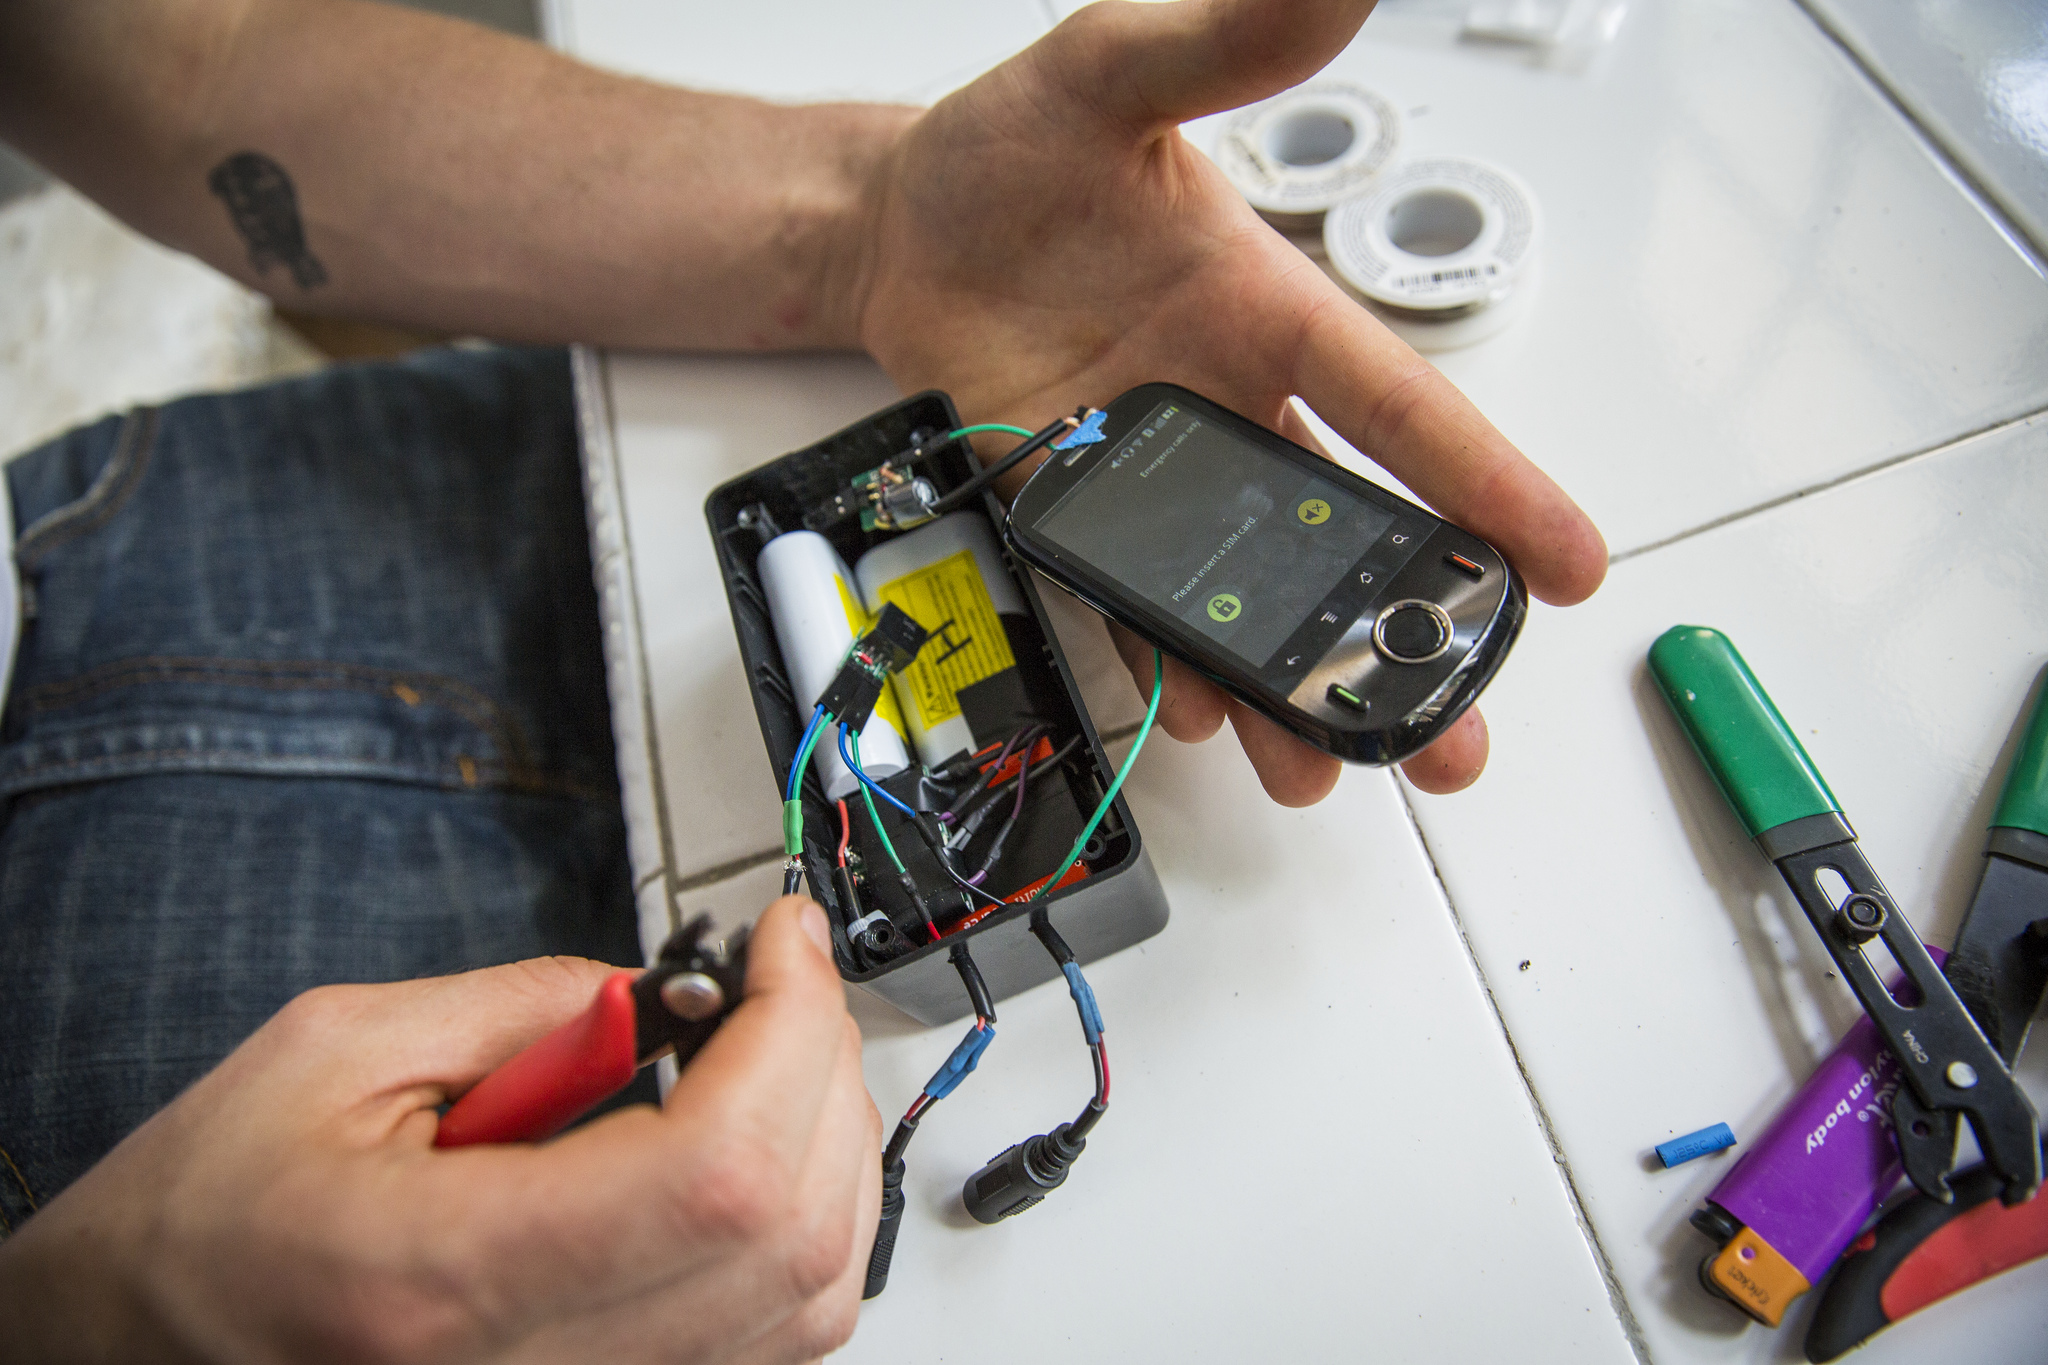
\includegraphics[width=0.8\textwidth]{device_inside}
  \caption{Inside of a device: Android phone, batteries, and various electrical components. Some solar charge controller PCBs can be seen in red at the bottom of the enclosure}
  \label{fig:device_inside}
\end{figure}
\newpage

The solar panel array consists of four petals, each of which has two solar panels on it. The panels are designed and patented by RFCx to work well under low light conditions such as those under the tree canopy. A single petal produces 1.5W of power under laboratory conditions. An individual petal can be seen in Figure \ref{fig:solar_petal}

\begin{figure}[H]
  \centering
  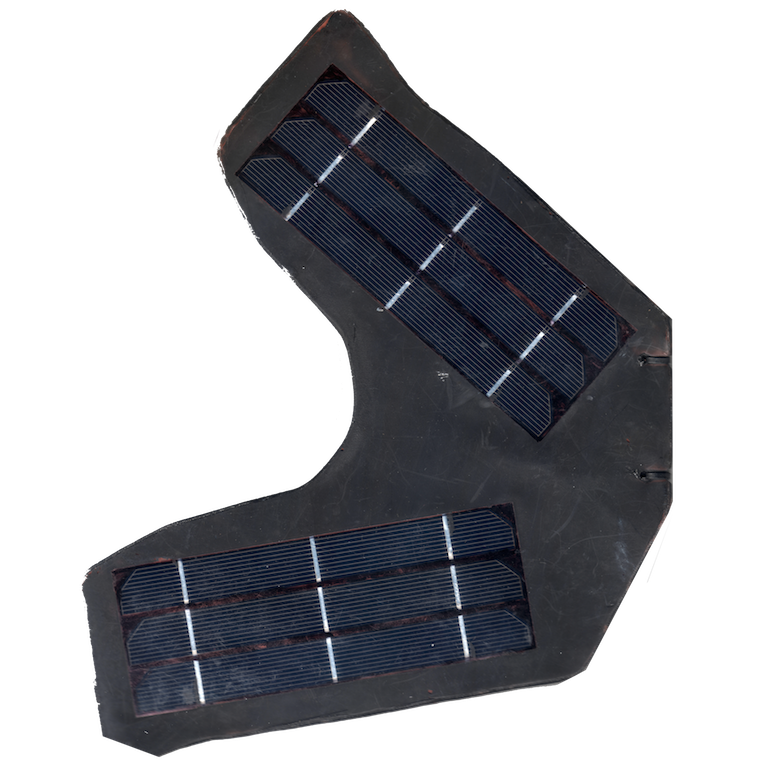
\includegraphics[width=0.8\textwidth]{solar_petal}
  \caption{A single solar petal consisting of two panels. Each panel is made from three strips of panel scraps left over from manufacturing at major solar panel companies, connected in series to produce a 1.5V output on each panel}
  \label{fig:solar_petal}
\end{figure}
\newpage

In regards to device enhancements, the principal objective of Project Necromancer is to merge all of the external electronics into a custom printed circuit board. This involves integrating the regulation circuitry and photovoltaic battery charge controller into a single board, and also introducing sensors for temperature, humidity, and power, a microcontroller, and other supporting electronics. The power, temperature, and humidity diagnostics will be sent from the microcontroller to the Android phone via a USB connection. Relaying the collected diagnostic data to the server is possible with the existing framework but is outside of the scope of this project. Instead, the collected data will be displayed for testing and verification purposes. A block diagram of the designed system is shown below in Figure \ref{fig:hldia}.

\begin{figure}[H]
  \centering
  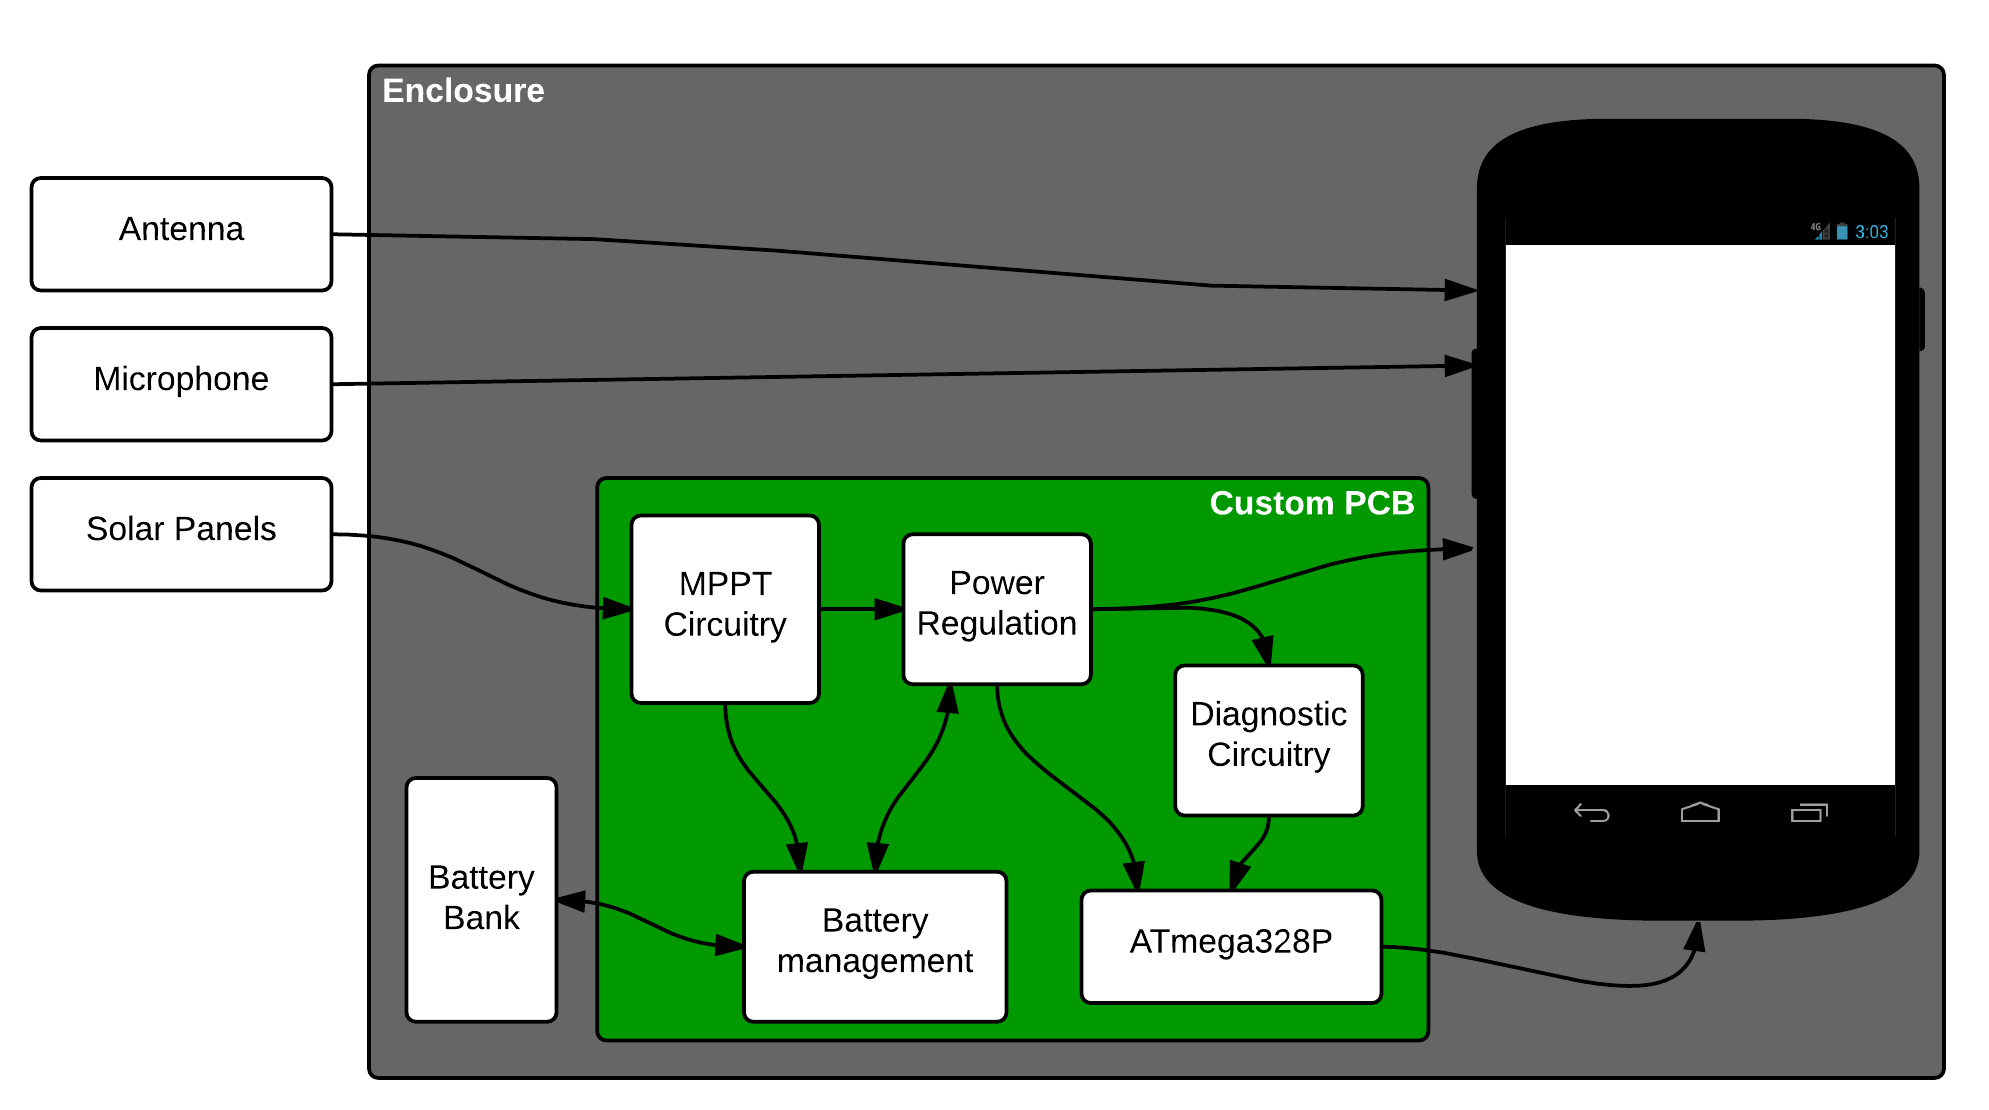
\includegraphics[width=0.8\textwidth]{Highlevel}
  \caption{High Level Functional Diagram of the Major Components}
  \label{fig:hldia}
\end{figure}
\newpage

On the phone, an app called RFCx Sentinel monitors the incoming diagnostics, displaying them to a screen, logging them to a file, and perhaps in the future transmitting them along with the audio data to the server. The RFCx Sentinel Application was developed by our team for the purpose of this project. An actual screenshot of the Sentinel application receiving data from a microcontroller is shown below in Figure \ref{fig:sentscrn}. In addition, although outside of the scope of this project, different audio compression schemes may be investigated if time allows.

\begin{figure}[H]
	\centering
	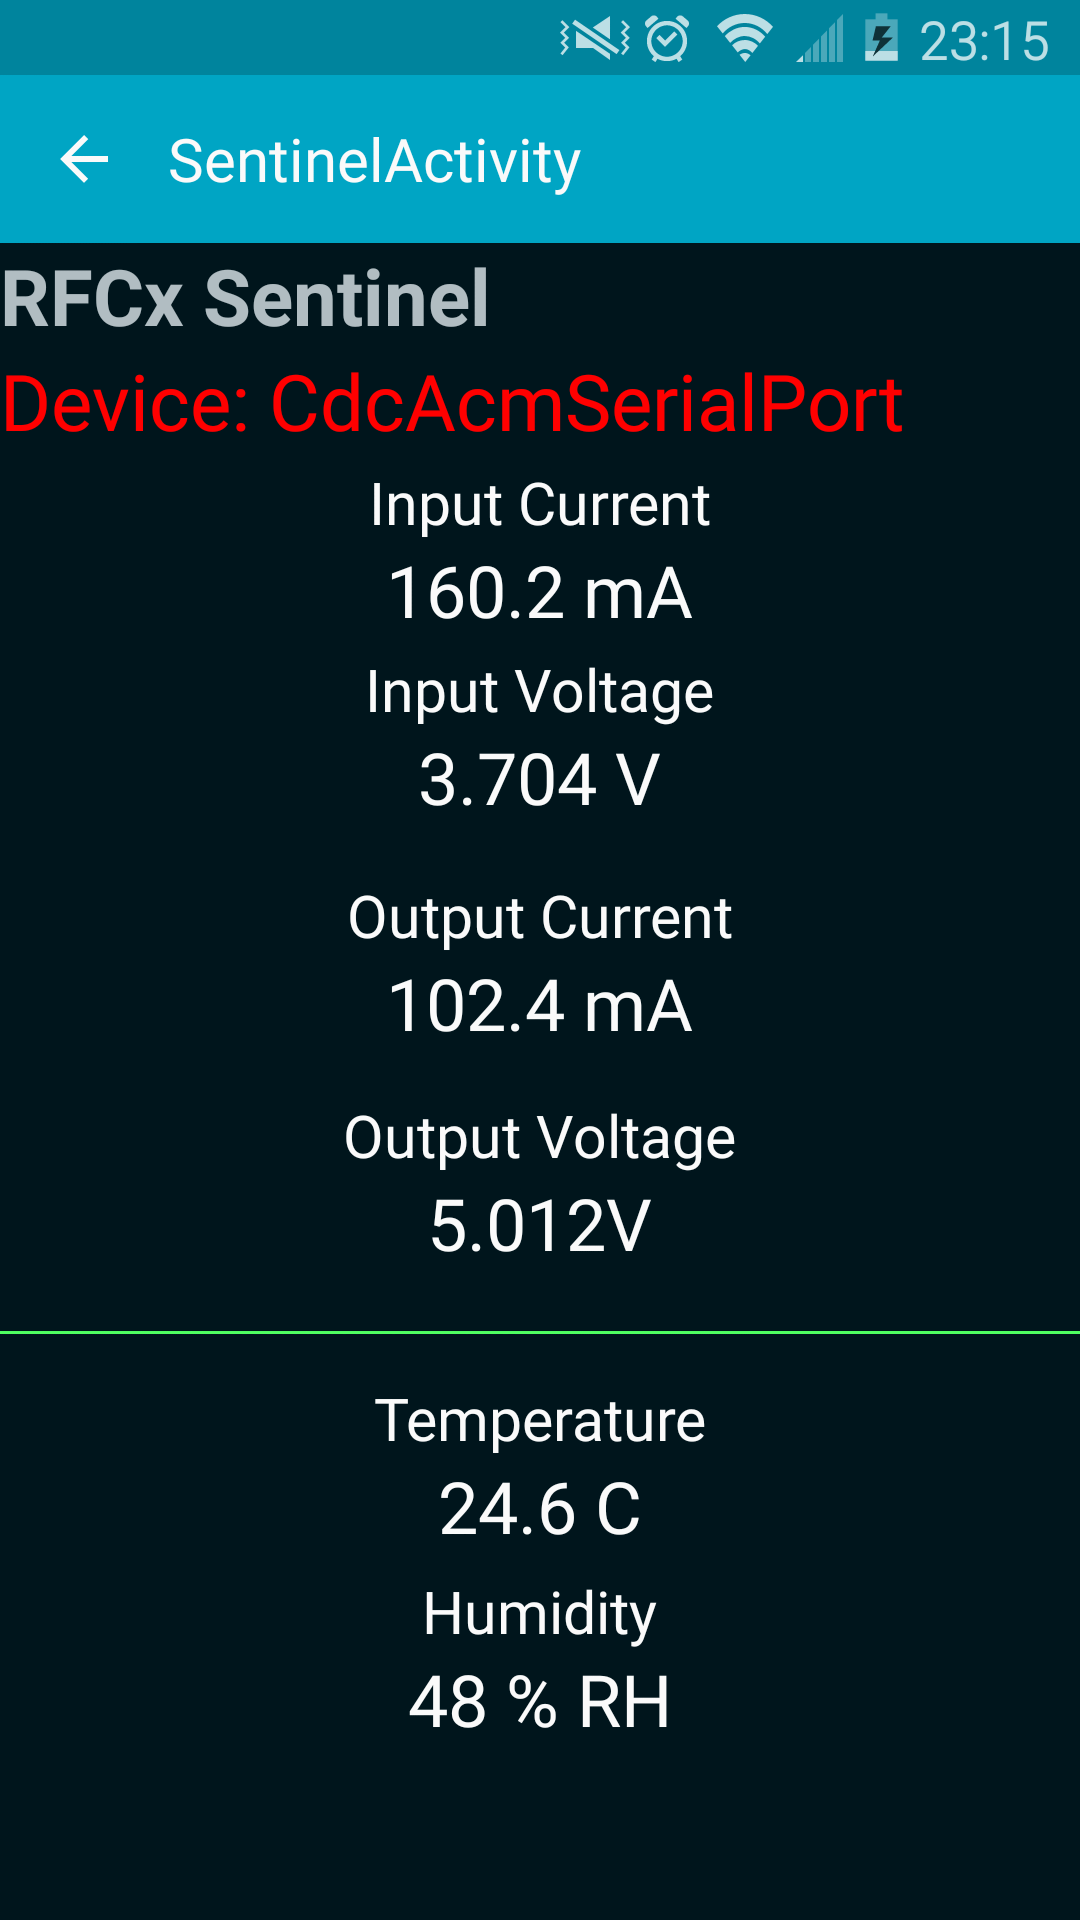
\includegraphics[width=0.4\textwidth]{RFCxSentinelScreenshot}
	\caption{Actual RFCx Sentinel App Screenshot}
	\label{fig:sentscrn}
\end{figure}
\newpage

%%%%%%%%%%%%%%%%%%%%%%%%%%%%%%%%%%%%%%%%%%%%%%%%%%%%%%%%% REQUIREMENTS %%%%%%%%%%%%%%%%%%%%%%%%%%%%%%%%%%%%%%%%%%%%%%%%%%%%%%%%%
\section{Requirements and Functional Specifications} \label{sect:requirementsandspec}
This section is organized by external and internal interfaces, with subsections in each for both hardware and software requirements.

\subsection{External Interfaces Requirements} \label{sect:externinterface}
This section addresses the requirements of the enhanced device pertaining to its external interfaces. External interfaces are defined as components of the device interacting with something outside of the device enclosure, including the antenna, microphone, solar panels, and GSM data communication. The possibility of compression is included under external interfaces because it directly relates to the sending of data outside of the device to the server.

\subsubsection{Hardware} \label{sect:hardware1}
\begin{enumerate}[align=left,leftmargin=*, labelindent= 0em, label=\textbf{Requirement \thesubsubsection.\arabic*.}, itemindent=0em]

\item \label{HWa} The device shall not exceed the existing power consumption and should reduce power consumption by at least 10\%.
\item \label{HWb} The interface with the phone shall consist of a USB connection for power and data, a 3.5mm microphone connection via the standard audio jack, and a connection to the external antenna via the existing antenna cable.
\item \label{HWc}The device shall use the existing external microphone and antennae
\item \label{HWd} Shielding techniques should be investigated to reduce the GSM audio interference noted by Topher White in the audio recordings.
\item \label{HWf} Camouflage color scheme may be used to conceal the device from loggers.  Additional camouflage features may be added so long as those features do not cover the solar panels.
\item \label{HWg} A simple assembly process shall be well documented with illustrations.

\baselinestretch
To verify \ref{HWg}. a sample group of people with varying skill levels will be asked to provide feedback on the assembly process and will be timed. The assembly times will be compared with current assembly times.

\item \label{HWh} The assembly and installation documentation may be translated into Spanish, French, and/or Portuguese.
\end{enumerate}
\subsubsection{Software} \label{sect:software1}
\begin{enumerate}[align=left,leftmargin=*, labelindent= 0em, label=\textbf{Requirement \thesubsubsection.\arabic*.}, itemindent=0em]
\item \label{SWa} The algorithm used to compress the audio signal may be compared to other existing algorithms and may be changed as such depending on the outcomes of comparative testing.

\baselinestretch
To verify \ref{SWa}, audio will be recorded and compressed using multiple algorithms including the current algorithm. An infographic hosted on RFCx’s website, shown in Figure 2 illustrates the flow of data that is collected from the phone and analyzed on the server.
\end{enumerate}

\subsection{Internal Device Requirements} \label{sect:internaldev}
This section addresses the requirements of the enhanced device pertaining to its internal interfaces and software. Internal here is defined as anything inside of the device enclosure, including but not limited to the Android phone, batteries, custom PCB, and supporting electronics.

\subsubsection{Hardware} \label{sect:hardware2}
\begin{enumerate}[align=left,leftmargin=*, labelindent= 0em, label=\textbf{Requirement \thesubsubsection.\arabic*.}, itemindent=0em]
\item \label{HW1}The PCB shall consist of battery management circuitry, the power regulation circuitry, power interface to the phone, power monitoring circuitry, as well as the microphone interface.

\baselinestretch
To verify \ref{HW1}, SPICE will be used to simulate the power charging circuitry to obtain power consumption and efficiency calculations. The manufactured and assembled board will then be subjected to a load test in a lab setting.

\item \label{HW3}There should be a low power microcontroller included on the PCB that communicates with the Android phone, sending it diagnostic information about components on the PCB. This will be used to monitor power consumption and provide external control of peripherals through the Android Debug Bridge protocol over USB. Extra general purpose pins of the microcontroller should be easily accessible for interfacing with future hardware.

\baselinestretch
To verify \ref{HW3}, simple packets will be sent from the microcontroller to the phone. These packets can be verified with debug tools or simple programs on the microcontroller and the phone. A debug serial port may be included as a peripheral to the microcontroller to aid in debugging. Any analog values read by the microcontroller will be verified with shop equipment.

\item \label{HW4} The monetary cost of the device, not including the solar panels, shall not exceed 25\% more than the current device cost, also not including the solar panels. The current cost of the solar panels has been quoted at \$200 and the rest of the device has been quoted at \$200. Increases in monetary cost above the current cost and below 125\% of the current cost are for enhancements in functionality (i.e. the PCB, etc.) and reductions in assembly time.

\end{enumerate}
\subsubsection{Software} \label{sect:software2}
\begin{enumerate}[align=left,leftmargin=*, labelindent= 0em, label=\textbf{Requirement \thesubsubsection.\arabic*.}, itemindent=0em]
\item \label{SW1}The microcontroller software should be capable of bi-directional communication between itself and the Android phone.
\item \label{SW2}The microcontroller software should be capable of communicating power usage diagnostics to the phone over the ADB protocol.
\item \label{SW3}An Android companion application may be capable of reporting power diagnostics from the microcontroller for testing and debugging.
\item \label{SW4}There shall be a header on the PCB to program the microcontroller.
\end{enumerate}

%%%%%%%%%%%%%%%%%%%%%%%%%%%%%%%%%%%%%%%%%%%%%%%%%%%%%%%% JUSTIFICATION %%%%%%%%%%%%%%%%%%%%%%%%%%%%%%%%%%%%%%%%%%%%%%%%%%%%%%%%%
\section{Component Justification} \label{sect:justification}
This section describes each component of the PCB in detail and gives justifications for their selection and a discussion of alternative choices that were considered. Along with the individual requirements of each device, a driving factor in device selection was the physical package of the IC; there should be no component that the end user cannot afix to the PCB without common soldering equipment.

\bigskip
The following is a list of the main ICs that comprise the PCB and are outlined in this section:
\begin{description}[font=$\bullet$\scshape\bfseries]
\item[Atmel ATMega328P]: 8-bit AVR microcontroller (Appendix \ref{fig:atmeldat})
\item[SPV1040 Max Point Power Tracker]: Solar power controller and lithium-ion battery charger (Appendix \ref{fig:spvdat})
\item[ADS1015]: External 4-input 12-bit Analog-to-Digital Converter, $I^2 C$ communication (Appendix \ref{fig:adsdat})
\item[LM75BD]: Ultra Low Power Temperature Sensor,$\pm 2^{\circ}C$, $I^2 C$ communication (Appendix \ref{fig:lm75dat})
\item[(Optional) HIH6130]: 14-bit resolution Humidity and Temperature Sensor with accuracy of $\pm5$\% Relative Humidity and $\pm 1^{\circ}C$, $I^2 C$ communication (Appendix \ref{fig:hihdat})
\item[FT230X]: FTDI USB-UART interface for USB serial communication (Appendix \ref{fig:ftdidat})
\item[BQ2057CTS]: Linear Battery Charge Management IC (Appendix \ref{fig:bq2057dat})
\item[LM61428]: Simple Switcher Boost Controller IC (Appendix \ref{fig:lmrdat})
\item[SM72238]: Micropower Fixed 3.3V LDO (Appendix \ref{fig:sm72dat})
\item[LTC6800]: Rail-To-Rail Input and Output Instrumentation Amplifier (Appendix \ref{fig:ltc6800dat})
\item[LTC4412]: Low loss powerpath controller (Appendix \ref{fig:ltc4412dat})
\end{description}

\subsection{Microcontroller} \label{sect:micro_just}
The ATmega328P microcontroller (Appendix \ref{fig:atmeldat}) was chosen as the microcontroller for the PCB. Many aspects were considered when choosing a microcontroller, including power consumption, available interfaces, availability of code samples, community support, ease of programming, and package size.

\bigskip
To this end, the ATmega328P is a logical choice; it is the microcontroller used by the popular Arduino platform, which means there are a multitude of code samples to reference for most any project. In addition, the 328P has a \textit{picopower} deep sleep mode, which consumes under 0.1$\mu$A of current. Unlike many options, the 328P has an easy to solder TQFP package. It is also is easily programmed by the use of an ICSP interface and does not require expensive hardware programmers or debuggers, as is the case for the Freescale KL25Z, which was also considered but requires a JTAG programmer.

\bigskip
Another microcontroller considered was the Texas Instruments 16-bit RISC MSP430. This microcontroller is the most expensive, draws the highest current in active and sleep modes, and requires an external tool to program.

\bigskip
USB communication was another concern when choosing a microcontroller. Similar MCUs that included on-board USB interfaces were also considered, but none could be found that offered the simple package, deep sleep mode, and $I^2 C$ communication. $I^2 C$ communication is needed to communicate with the analog-to-digital converter and temperature/humidity sensors.

\subsection{MPPT} \label{sect:mppt_just}
The SPV1040 Max Point Power Tracker (MPPT) (Appendix \ref{fig:spvdat}) was chosen to perform the solar charge management. A driving factor in choosing the SPV1040 was that RFCx had already established a supplier and had many on-hand to ship us for prototyping. In addition, it has the advantage of being simpler to use than similar chips, like the Solar Magic SM72442, in that no $I^2 C$ communication is necessary to set and configure registers to perform the same function. Finally, the currently used MCP73871 chip (currently on an off-the-shelf Adafruit board) fails in both the physical package being difficult to assemble by hand (QFN package) when used alone, and being meant for only single-cell Lithium-Ion batteries. In addition, the MCP73871 does not use a true MPPT algorithm, but rather an approximation.

\subsection{MPPT Configuration} \label{sect:mppt_config_just}
The MPPT configuration makes a large difference in many aspects of the selection of other components. First, each MPPT can only handle 1.8A of current. Also, the input voltage of each MPPT must be much less than the desired output voltage for them to function properly. Depending on the configuration, the number of MPPT ICs can vary from 1 to 8, increasing cost, and the voltage and current characterstics vary depending on whether they are connected in series or in parallel.

\bigskip
The following figure (Figure \ref{fig:mppt_config2}) describes the chosen MPPT configuration. In this configuration, each petal, which consists of two 1.5V panels, has its panels connected in series, giving an output of 3.0V, at 1.5W. This results in a current of 500mA for each MPPT, which is well below the maximum. Each petal (four total) is then connected to its own MPPT, which is set to boost to 5.2V. The MPPTs are then connected in parallel.

\bigskip
Connecting multiple regulators in parallel can sometimes cause problems if one source is outputting a slightly smaller or larger voltage than the others. In most cases, the use of ballast resistors solves this problem. The footprint for a ballast resistor was chosen to be included in series with the output of each MPPT. The footprint will be first populated with a 0$\Omega$ resistor, and the current will be monitored from each MPPT to ensure they are sharing the load correctly. If they are not, the footprint will be populated with a $25m\Omega$ ballast resistor, and the same test will be performed.

\begin{figure}[H]
  \centering
  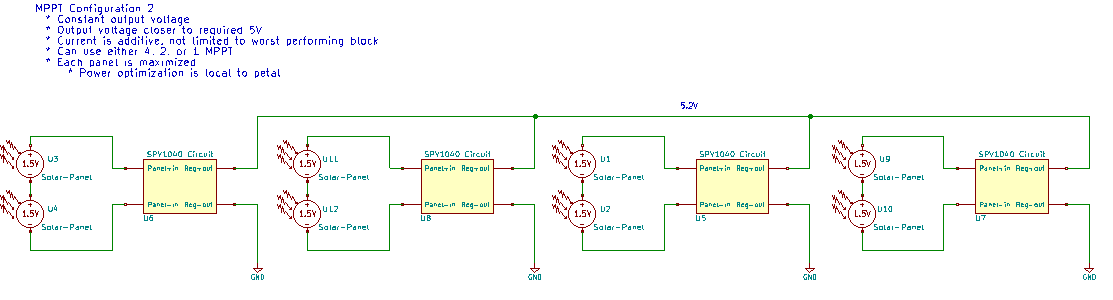
\includegraphics[width=1.0\textwidth]{MPPTConfig2}
  \caption{Four MPPTs are connected in parallel with the input being the series connection of each panel within a single petal}
  \label{fig:mppt_config2}
\end{figure}

This configuration offers many benefits. First, the panels on a single petal can be either connected in series or in parallel. Since the SPV1040 can handle up to 1.8A, even when connected in parallel the petal will only produce a maximum of 1A. The input voltage to the MPPT can be either 1.5V (panels in parallel) or 3.0V (series), and the MPPT's internal boost regulator will still produce 5.2V. This allows for testing configurations where all petals have their panels connected in parallel, all in series, or a combination of both under different lighting conditions to see which performs the best without modifying the PCB in any way.

\bigskip
In addition, this configuration localizes the power tracking to an individual petal. Rather than maximizing the entire array, localizing to each petal allows for some petals to be in direct sunlight while others are in shade and each MPPT will react accoringly.

\bigskip
Furthermore, this configuration could be easily adapted to using less MPPTs if needed (to reduce cost, for example). To use two MPPTs, for example, instead of four, two of the ICs would simply not be populated and pairs of petals would be connected in parallel externally and connected to the two populated MPPTs. This is shown in Figure \ref{fig:mppt_config3}.

\bigskip
Finally, as required by the SPV1040, the input voltage will always be much less than the output in this configuration. The input voltage will be either 1.5V (parallel panels) or 3.0V (series), well below the 5.2V output.

\bigskip
Two other configurations that were considered are shown below. In the first alterate configuration, in Figure \ref{fig:mppt_config1}, two pairs of MPPTs connected in series are then connected in parallel. This has many drawbacks, including requiring a higher output voltage when it is not needed, and requiring the use of diodes to prevent current from backfeeding into the other MPPTs.

\begin{figure}[H]
  \centering
  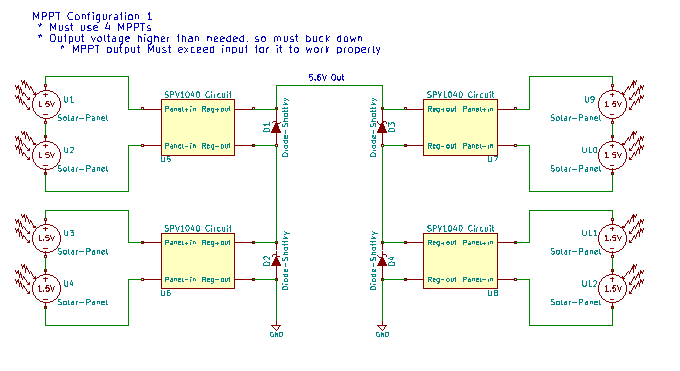
\includegraphics[width=1.0\textwidth]{MPPTConfig1}
  \caption{Two pairs of MPPTs are first connected in series, then in parallel, requiring the use of feedback diode protection and resulting in a higher than needed output voltage which must then be bucked down}
  \label{fig:mppt_config1}
\end{figure}

The second alternate configuration, in Figure \ref{fig:mppt_config3}, is really the same as the chosen one, but using two MPPTs instead of four as described above.

\begin{figure}[H]
  \centering
  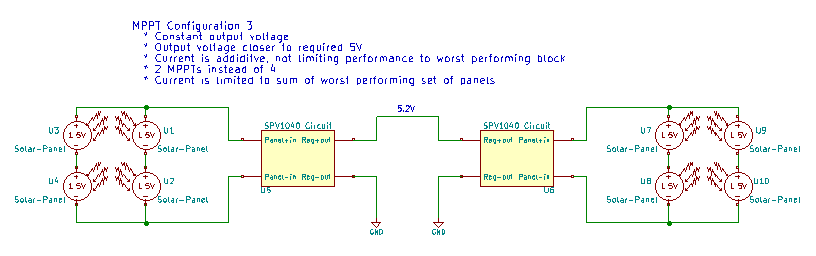
\includegraphics[width=1.0\textwidth]{MPPTConfig3}
  \caption{Chosen configuration but with two MPPTs instead of four. Results in less control but saves the cost of two ICs and the supporting circuitry of each}
  \label{fig:mppt_config3}
\end{figure}

\subsection{ADC} \label{sect:adc_just}
The ADS1015 external ADC (Appendix \ref{fig:adsdat}) was chosen to perform analog-to-digital conversions for the power sensing. The ATmega328P does not have a strong internal ADC, being only 10-bit resolution, and the ADS1015 is easy to communicate with via $I^2 C$. The ADS1015 consumes less than 150$\mu$A, has 12-bit resolution, and supports four single-ended analog inputs, which will be used to monitor input current, input voltage, output current, and output voltage on the PCB.

\bigskip
$I^2 C$ supports multiple devices in parallel, so only two of the ATmega328P's six analog pins are used. This frees the other four for future use, which is a major advantage of using an external ADC.

\subsection{Temperature and Humidity Sensor} \label{sect:temp_just}
The LM75BD (Appendix \ref{fig:lm75dat}) was chosen as the temperature sensor.  The LM75 is a super low power temperature sensor with an accuracy of $\pm2^{\circ}C$. It uses less than 300uA during peak transmission, and costs under \$1.

\bigskip
An alternative sensor prodiving both temperature and humidity measurements, the HIH6130 (Appendix \ref{fig:hihdat}), was also considered. Also using $I^2 C$ and also being low-power, the only real drawback is the price, at nearly \$14. For this reason the LM75BD was chosen, but the footprint for the HIH6130 will be included but unpopulated on the board as an option to the end user.

\bigskip
Other lower-cost humidity and temperature sensors were investigated, such as the DHT11 and DHT22. The DHT11 is affordable, at around \$5, but has a limited range of 0-50$^{\circ}C$. The DHT22 has the range required and is accurate, but costs almost as much as as the HIH6130 at around \$9. Both the DHT11 and DHT22 are not $I^2 C$, but rather use the one-wire-interface which requires elaborate timing to get the correct data, and take up another pin on the microcontroller. In addition, Adafruit and Amazon were the only places that stock the DHT22, neither of which offer the reliability or quantity of sources like Digikey or Mouser.

\bigskip
In addition to other $I^2 C$ temperature sensors, traditional analog sensors were also considered. The popular LM35 analog sensor, despite having less features than the LM75BD, costs over twice as much, at \$1.75.

\bigskip
The LM75BD is accurate within $\pm3^{\circ}C$ from $-25$ to $+100^{\circ}C$ and within $\pm2^{\circ}C$ from $-55$ to $+125^{\circ}C$. The HIH6130 can operate in the temperature range of $-25^{\circ}C$ to $85^{\circ}C$ and from 10\% to 90\% Relative Humidity (RH) with an accuracy of $\pm1^{\circ}C$ and $\pm5$\% RH.

\subsection{FTDI} \label{sect:ftdi_just}
The FT230X FTDI chip (Appendix \ref{fig:ftdidat}) was chosen for the UART to USB interface between the microcontroller and the Android phone. FTDI is widely used and supported, and, unlike similar devices like the Arduino's CDCACM, does not require another microcontroller to be added, configured, and flashed with software. In addition, the RFCx Sentinel application, which uses the open source usb-serial-for-android library, readily supports FTDI. Serial USB communication has already been achieved using an ATmega328P MCU, a similar FTDI chip, and the Sentinel app.

\subsection{Battery Management} \label{sect:battery_just}
Battery management is important for the ability to reclaim and potentially fix a damaged battery, and also to prevent potential fire hazards. Being in a hot climate and surrounded by ample fuel for a large-scale forest fire, battery management was chosen to be included in the design. The bq2057CTS battery charge management IC (Appendix \ref{fig:bq2057dat}) was thus chosen to control the charging of the Lithium-Ion batteries. It is designed for both single and dual-cell battery packs, and combines current and voltage regulation, charge status indication, and charge rate auto compensation.

\bigskip
Although battery management \textit{can} be done in software with the microcontroller, the amount of work required to do so is disproportional to any benefits you may gain. In fact, by performing battery management on the microcontroller, those writing the software take responsibility for any damage to the batteries, or even substantial damage such as a fire. This is in contrast to using an off-the-shelf, proven solution such as the bq2057CTS.

\subsection{Power Path Management} \label{sect_pow_just}
To manage the power selection between the solar panels and the batteries, a power path management solution was required. This was required because while the batteries are being charged the rest of the circuit should not draw from them. If the rest of the circuit draws from them while they are being charged, the battery charge management IC could get confused and damage the batteries by over charging or under charging. A diode-ORed configuration, in which power sources are ORed together via a near ideal diode($0.02V_f$), selects the source with the higher voltage. The LTC4412 (Appendix \ref{fig:ltc4412dat}) was chosen to perform this power path management. The ideal diodes are implemented externally with a FZT788B P-Channel MOSFET (Appendix \ref{fig:ftzdat}). This IC also has a very low quiescent current, below $1.15\mu A$.

\subsection{Power Regulation} \label{sect:reg_just}
The LMR61428(Appendix \ref{fig:lmrdat}) Step-Up Voltage regulator was chosen because of its price, package, and performance. It is important for all of the ICs on this board to be in a package that the end user can assemble with without the aid of more advanced PCB assembly equipment such as solder paste/stencils and ovens. Also, some of the other buck/boost controllers required a much higher input voltage when the load current was around 500mA. The LMR61428 requires less than 2V, which is possible even when drawing from the batteries. Since this is design is for a remote device powered from batteries and solar power, quiecent current is a concern as well. The LM61428 only draws 80mA during operation.

\bigskip
The Texas Instruments SM72238 Micropower fixed 3.3V linear voltage regulator was chosen to regulate the 3.3V line because it has a very low dropout voltage of around 380mV at the max current draw of 100mA.

\subsection{Current Sensing} \label{sect:cur_just}
The LTC6800 precision instrumentation amplifier (Appendix \ref{fig:ltc6800dat}) was chosen to perform current sensing. This instrumentation amplifier operates rail-to-rail on the input and output, which provides a larger window to sense the voltage across the sense resistor. A sense resistor value of 0.010$\Omega$ was chosen to provide minimal power dissipation. Although very small, since the leakage current into the opamp is also extremely small (on the order of 1nA), the trace resistance, which is approximately 0.035$\Omega$, is not a concern. The LTC6800 also draws very little current. Under no load the LTC6800 draws a maximum of 1.3mA.

\subsection{PCB Size} \label{sect:pcb_just}
Two options were considered for the physical form of the PCB. The first was only large enough for the components on the board, and would be mounted in the enclosure alongside the batteries and phone. The second design, which was chosen, uses a PCB slightly larger than the size of the phone itself. This allows for the entire phone and PCB to be attached and easily removed/inserted into the enclosure as one piece. The PCB design is shown in Section \ref{sect:pcbdesign}.

\subsection{Heat Dissipation} \label{sect:heat_just}
Multiple solutions were explored for dissipating heat inside the enclosure. These include drilling holes into the enclosure, putting fans in the enclosure to control airflow in and out of the enclosure, and using a heat sink.

\bigskip
Using a heat sink was chosen as the best design alternative for heat dissipation. Drilling holes in the enclosure can allow water, insects and dust to enter the enclosure. A wire mesh over the holes could be used to keep insects out of the enclosure, but water and dust could still get into the enclosure and damage the electronics. Running fans in the device creates a sound in a similar frequency range to the chainsaw noise the device is trying to detect. This can cause false detection of a chainsaw by the RFCx server.

\bigskip
A heat sink also requires a hole to be drilled into the enclosure for the heat sink to reach outside of the enclosure. This opening will be sealed with caulk or by other methods to prevent water, insects and dust from entering the enclosure. The battery cover on the phone will be removed and thermal paste will be used between the phone battery and the PBC, and between the PCB and the heat sink. This will allow heat to dissipate out of the enclosure and help keep the phone attached to the PCB and the PCB attached to the heat sink. Vias in the PCB will help heat to transfer through from the phone to the heatsink. The heatsink implementation is shown in Section \ref{sect:heatsinkimplementation}.

%%%%%%%%%%%%%%%%%%%%%%%%%%%%%%%%%%%%%%%%%%%%%%%%%%%%%%%%%%%% DESIGN %%%%%%%%%%%%%%%%%%%%%%%%%%%%%%%%%%%%%%%%%%%%%%%%%%%%%%%%%%%%
\section{System Design} \label{sect:sysarch}
\subsection{Hardware Design} \label{sect:hardwaredesign}

\subsubsection{Power Sources}
The system is powered from eight solar cells that have been manufactured by RFCx. These solar panels have been reported to have an open circuit voltage of 1.6V and produce an average of 0.75W each under laboratory conditions. The other power sources on board are two dual-cell 4400mA/Hr lithium-ion (Li-ion) battery packs. As discussed in the MPPT configuration justification, the solar panels will be configured in a way that a pair on an individual petal may be wired in either series or parallel. The pairs will be wired how the end user would like them and the remaining wires will be connected to a terminal block with screw/leaf spring wire termination on the PCB, which will be powering the MPPT controllers. This is illustrated in Figure \ref{fig:mpptsol}.

\begin{figure}[H]
	\centering
	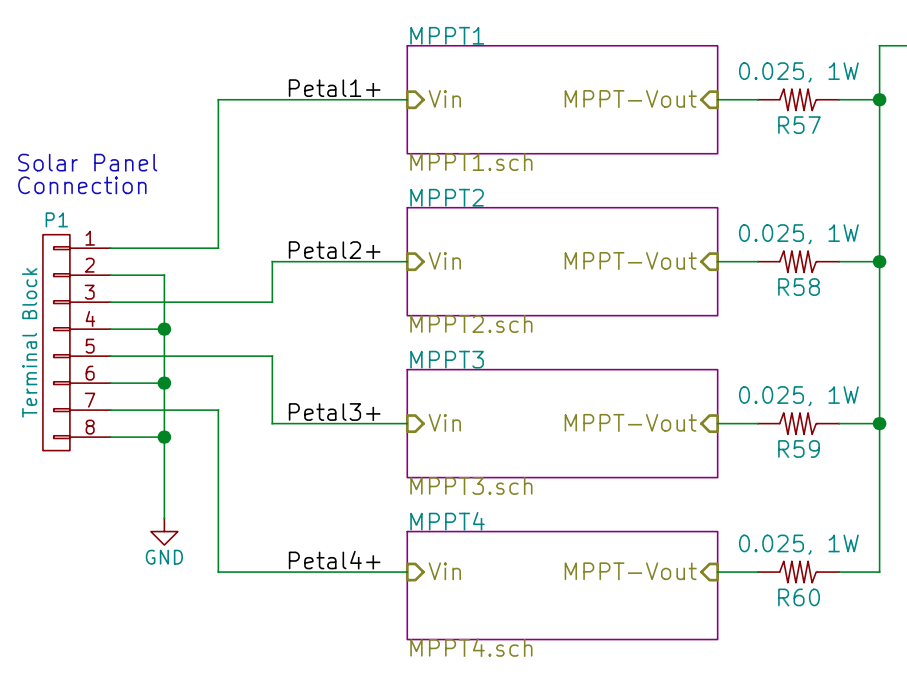
\includegraphics[width=0.8\textwidth]{MPPTblocks}
	\caption{MPPT and Solar Panel Interface}
	\label{fig:mpptsol}
\end{figure}

With this configuration a configurable output voltage of 5.2V, the maximum of the SPV1040, will be obtained at an average of about 1.15A, yeilding an input power of about 6W.

\subsubsection{Solar Charging}

A Max Point Power Tracker (MPPT) increases efficiency by adjusting the current and voltage of the output to achieve the maximum power. The SPV1040 will regulate the solar cell voltage up to 5.2V. From the MPPT the battery management circuitry, the 3.3V line, and the 5V line is powered. The MPPT circuit is shown in Figure \ref{fig:singlemppt}.

\begin{figure}[H]
	\centering
	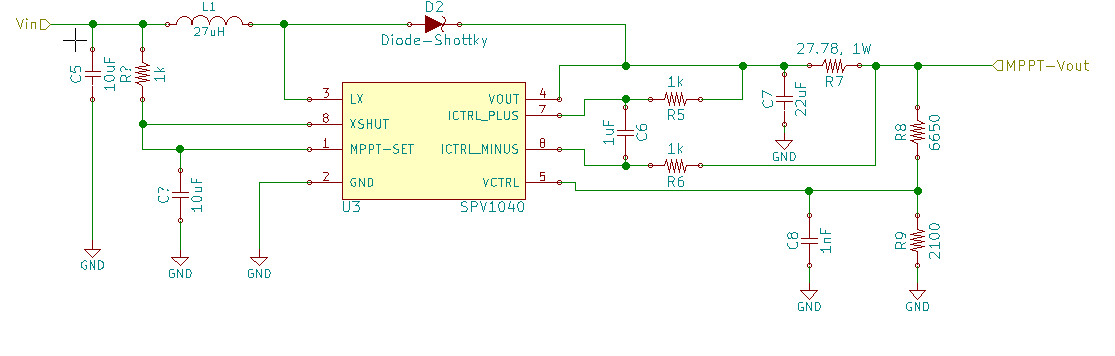
\includegraphics[width=0.8\textwidth]{singlempptcircuit}
	\caption{Single SPV1040 MPPT Circuit}
	\label{fig:singlemppt}
\end{figure}

\bigskip
The input capacitor's purpose is to reduce voltage ripple. It was calculated that this capacitor must be greater than $14.3\mu F$. The time constant of the resistor and capacitor on the \textit{MPPT SET} pin of the SPV1040 IC must be less than or equal to the maximum power point tracking time ($T_{MPPT} \cong 1ms$). It is recommended that the resistor be set to $1k\Omega$. This means that the capacitor must be less than $10\mu F$. The inductor selected was based on the maximum input voltage and current produced by the solar petals. The inductor value was calculated to being greater than or equal to $8.5\mu H$. The saturation current for the inductor must also be greater than 1.8A, which is the limit of the SPV1040. The output voltage capacitor was chosen based on the short circuit current of the solar petals and the maximum voltage ripple. The output voltage capacitor must be greater than $142\mu F$ so $150 \mu F$ was chosen. This was calculated with a maximum output ripple voltage of 0.01V. There are two resistors that divide the output of the SPV1040 and provide feedback to the controller. These resistors were calculated to be $76.8k\Omega$ and $24.3k\Omega$. This divides the desired maximum output voltage of 5.2V to 1.25 at the voltage sensing pin. The capacitor on the $V_{CTRL}$ pin of the SPV1040 is needed to reject noise sensed by the pin. This was calculated to be around $45.2\mu F$. The voltage drop across the sense resistor is compared to the 50mV internal reference. The sense resistor is calculated to be around $27m\Omega$. Since there may be some noise from the switching, there is a filter on the sense pins, \textit{Ictrl\_+} and \textit{Ictrl\_-}. It is recomended that the inline resistors are $1k\Omega$ and the capacitor between the two is $1\mu F$. A Schottky diode is placed between the \textit{Lx} and \textit{Vout} pins of the SPV1040. The \textit{Diodes Incorporated} 1N5819HW Schottky diode meets the suggested criteria. It has a forward voltage drop of 450mV and a non repetitive peak current of 25A. The calculations for these components can be found in Appendix \ref{app:spvcalcs}.

\subsubsection{Battery Management}

The two dual-cell Lithium-Ion batteries are each managed by a bq2057CTS. Figure \ref{fig:batman} shows the battery management circuitry for one of the 2-cell battery packs. This IC provides voltage and current regulation, battery conditioning, temperature monitoring, charge termination, charge status indication, as well as charge-rate compensation. The charging is started in the constant voltage phase and stops when the current falls bellow the current termination threshold. The bq2057 inhibits charging until the battery temperature is in the user defined range. This range is defined in this circuit with the $49.9k\Omega$ resistor \textit{R24} as an upper bound of 50$^{\circ}C$. The PNP BJT pass transistor controls voltage and current regulation as well as providing protection from backfed current. Only the upper temperature bound is set because the device is not intended for cold environments. The charge rate compensation is set by resistors \textit{R18} and \textit{R22}. These values are outlined in the datasheet (Appendix \ref{fig:bq2057dat}) to set a proprietary charge compensation algorithm. The automatic charge compensation helps to charge the batteries faster and compensate for the battery pack's internal impedance.

\begin{figure}[H]
	\centering
	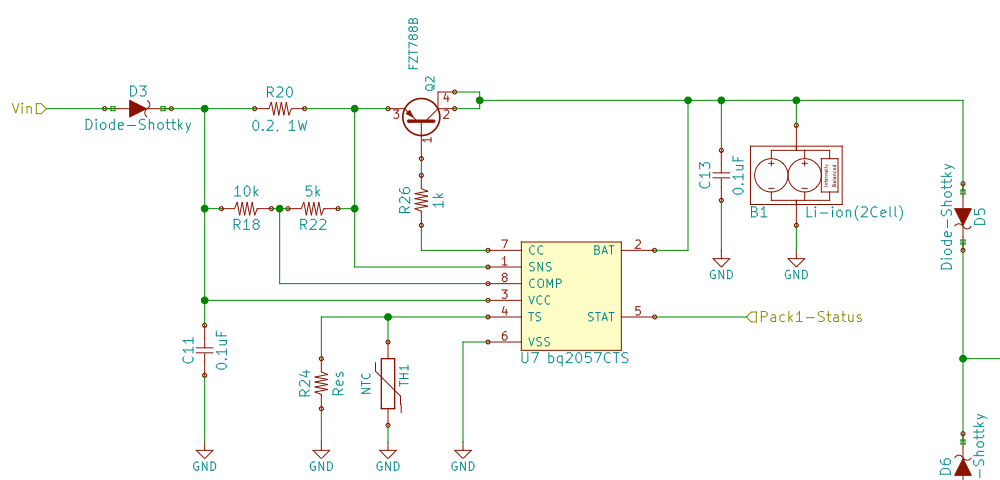
\includegraphics[width=0.8\textwidth]{BatteryManage}
	\caption{Battery Management Circuitry}
	\label{fig:batman}
\end{figure}

The calculations for the component selection for the battery management circuitry is included in Appendix \ref{sect:bqcalcs}.

\subsubsection{Voltage Regulation}

A diode-ORed power path management circuit was used to switch the power source that feeds the 3.3V and 5V regulation circuitry. This circuit is shown in figure \ref{fig:dored}.

\begin{figure}[H]
	\centering
	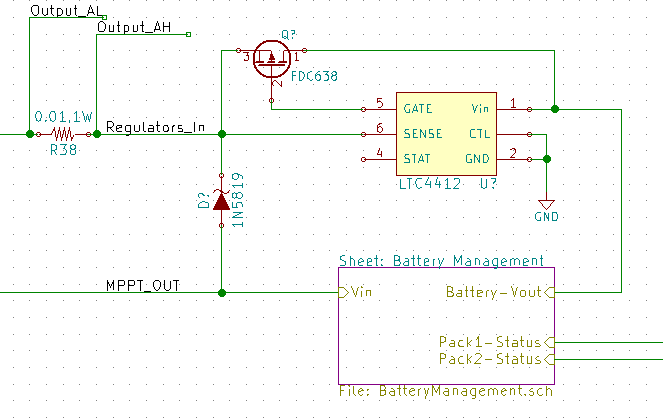
\includegraphics[width=0.8\textwidth]{DiodeOR}
	\caption{Diode Ored Circuit}
	\label{fig:dored}
\end{figure}

This circuit provides power path switching in under 100 $\mu$s, and there is virtually no dip in the output voltage during the switch. A dip of approximately 500mV was observed when using a transistor alone to simply switch between the two sources, as shown in the simulation figure in Appendix \ref{fig:doredsimres1}. With the diode-ORed topology, the switch is clean, as seen in the simulation figure in Appendix \ref{fig:doredsimres2}.

\bigskip
The LM61428 is a step-up voltage regulator that is configured to boost the input voltage to 5V at an output current of up to 1A. The output voltage of 5V is used to power the Android phone.

\bigskip
The layout of the 5V boost regulator can be seen in figure \ref{fig:ps5}.
\begin{figure}[H]
	\centering
	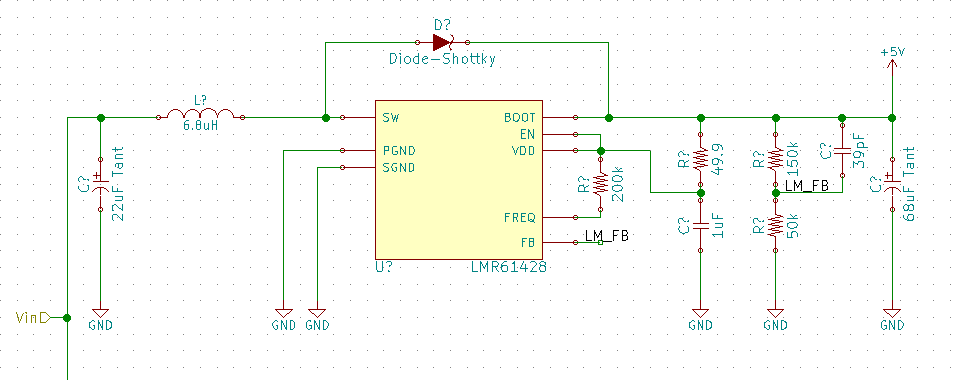
\includegraphics[width=0.8\textwidth]{PS5V}
	\caption{5V Voltage Regulation}
	\label{fig:ps5}
\end{figure}

\bigskip
A Texas Instruments SM72238 Micropower fixed 3.3V LDO is used to regulate the 3.3V line. The SM72238 has very low dropout, which is in range for the need of this application. The only external components required by the LDO are two low ESR 1uF capacitors on the input and output. The circuit can be seen in figure \ref{fig:sm722}.

\begin{figure}[H]
	\centering
	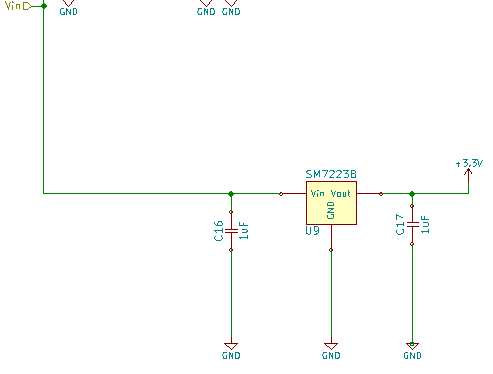
\includegraphics[width=0.8\textwidth]{PS33V}
	\caption{3.3V Voltage Regulation}
	\label{fig:sm722}
\end{figure}

\subsubsection{Input and Output Current and Voltage Sensing}

The ADS1015 is a 12-bit ADC that can communicate over $I^2 C$ with the microcontroller. This ADC will operate in single shot mode and then go back to sleep. The ADS1015 uses a $\delta\sigma$ ADC and can perform conversions at rates up to 3300 samples per second. The microcontroller will initiate a conversion over $I^2 C$ and be able to send the diagnostic to the phone for further processing. A code snippet can be seen below in Section \ref{sect:softwaredes}.

The LTC6800 instrumentation amplifier is used to sense the voltage across a known sense resistor. The input current sense circuit is configured to have a gain of around 80.5. The sense resistor has been selected to be 0.01$\Omega$. With this configuration the ADC will be able to sense the current with a resolution of 1mA/bit. The calculations for this section can be seen in Appendix \ref{app:cvsense}. The configuration of the current sense amplifier can be seen in Figure \ref{fig:AV}. The input and output voltage are sensed with simple resistor dividers that are fed to the ADC.
\begin{figure}[H]
	\centering
	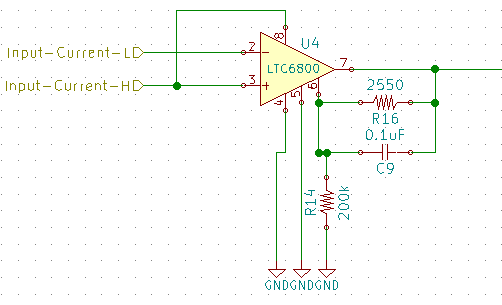
\includegraphics[width=0.8\textwidth]{AtoV}
	\caption{Current Sense Amplifier}
	\label{fig:AV}
\end{figure}

\subsubsection{Microcontroller}

The only supporting circuitry for the ATmega328P is the 6-pin in-circuit serial programming (ICSP) port, a 32kHz external crystal, and external pull up resistors on the $I^2 C$ communication lines. The 32kHz crystal is included for the real time clock. The real time clock is used so that the ATmega328P microcontroller can go into a sleep mode and wake up later to conserve power usage. The ATmega328P also requires an FTDI IC to communicate with the phone over USB. The microcontroller and surrounding circuitry is shown below in Figure \ref{fig:mcu}.
\begin{figure}[H]
	\centering
	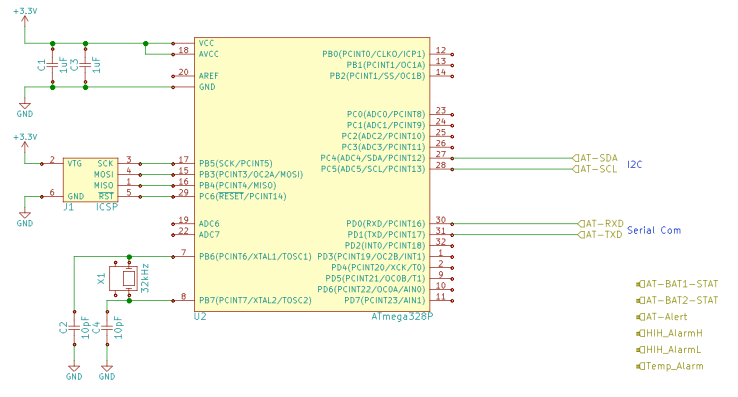
\includegraphics[width=0.8\textwidth]{Microcontroller}
	\caption{Microcontroller}
	\label{fig:mcu}
\end{figure}

\subsubsection{Temperature and Humidity}

Both the temperature sensor (LM75BD, Appendix \ref{fig:lm75dat}) and humidity/temperature sensor(HIH6130, Appendix \ref{fig:hihdat}) require minimum supporting circuitry to operate due to their internal clocks, internal analog-to-digital converters, and internal memory. The LM75, however, still requires a resistor network to set the $I^2 C$ address bits associated with the chip. As seen below in Figure \ref{fig:tandh}, resistors R51 to R56 are used to set the address bits. For each input, either the pull-up or pull-down resistor will be populated and the other will be populated with a 0$\Omega$ resistor to set the bit to either a logic 1 or 0.

\begin{figure}[H]
	\centering
	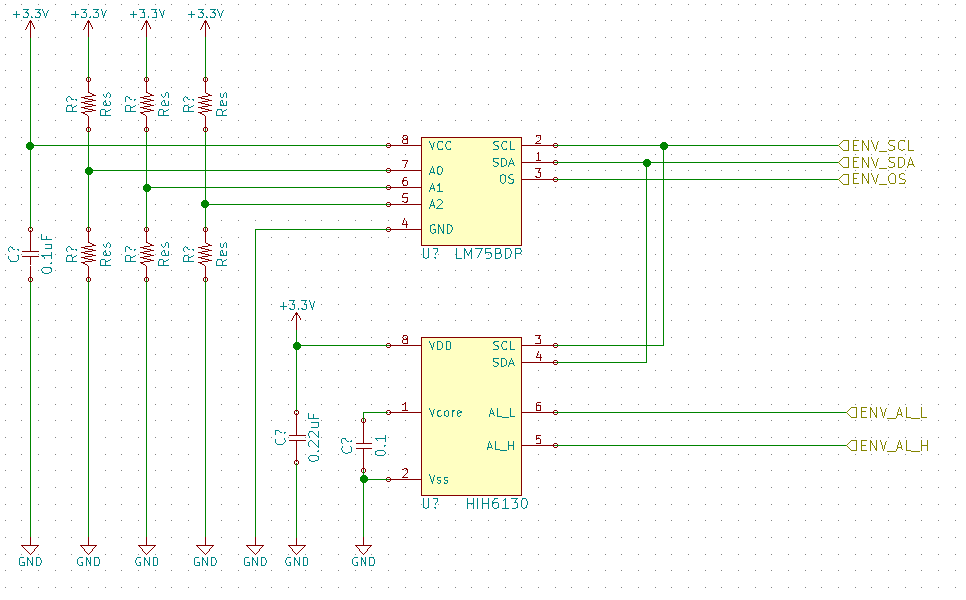
\includegraphics[width=0.8\textwidth]{temphumid}
	\caption{Temperature and Humidity Sensors}
	\label{fig:tandh}
\end{figure}

\subsubsection{PCB} \label{sect:pcbdesign}
The dimensions of the chosen PCB size is shown in Figure \ref{fig:pcbdimensions}. This size accomodates both the phone currently used, the Huawei Ideos U8180, with dimensions of \textit{4.09"} x \textit{2.16"} x \textit{0.54"}, as well as larger Android phones up to \textit{5"} x \textit{2.8"} x \textit{0.625"}. The dimensions of the phone relative to the PCB is shown in Figure \ref{fig:pcbphone}.

\begin{figure}[H]
	\centering
	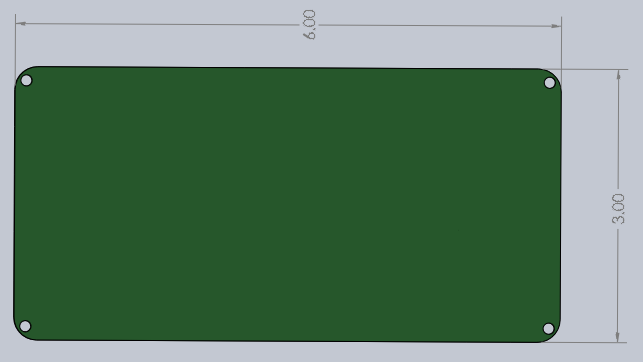
\includegraphics[width=0.8\textwidth]{PCB}
	\caption{PCB Dimensions}
	\label{fig:pcbdimensions}
\end{figure}

\begin{figure}[H]
	\centering
	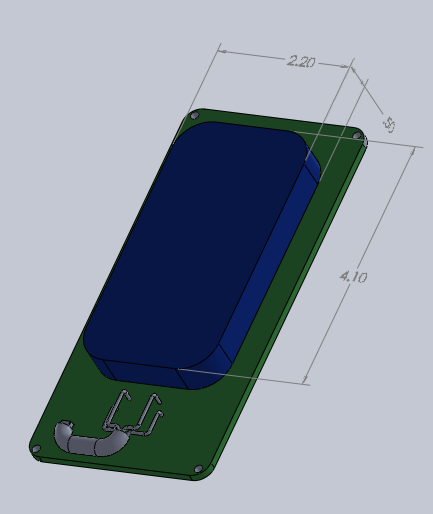
\includegraphics[width=0.8\textwidth]{PhoneAndPCB}
	\caption{PCB Dimensions}
	\label{fig:pcbphone}
\end{figure}

\subsubsection{Connectors}

The USB connection consists of a standard USB Micro A connector, soldered directly onto the board and is secured to the board as a strain-relief mechanism, which is shown in Figure \ref{fig:usbcable}. A standard 3.5mm audio cable is used to connect the microphone. The existing standard GSM antenna adapter is used to interface with the phone’s onboard GSM module.

\begin{figure}[H]
	\centering
	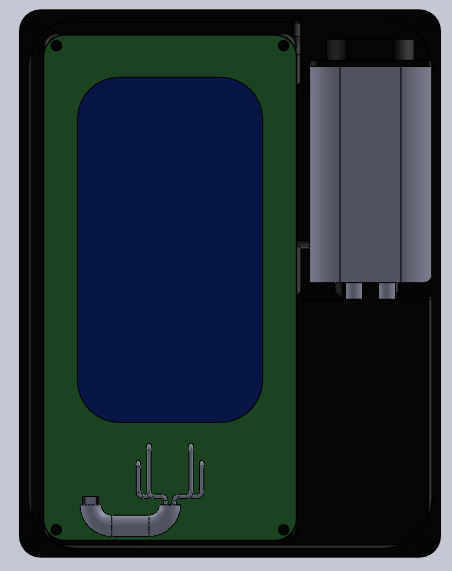
\includegraphics[width=0.8\textwidth]{Assembly1}
	\caption{USB Micro A Connector attached to the PCB with strain relief: A small flexible cable}
	\label{fig:usbcable}
\end{figure}

\subsubsection{GSM Interference}

The use of X2Y TDMA filtering capacitors will be tested to reduce the noise produced by the stopping and starting of GSM packets, which is in the audible range at ~217Hz. These capacitors are essentially a three node capacitive circuit that has two closely matched, low inductance capacitors in a single package. Manufacturer tests show a nearly flat response for a GSM handset close to an audio circuit. A pass-through 3.5mm microphone interface will be included to test the X2Y capacitors. The pass through circuit can be seen in figure \ref{fig:x2y}.

\begin{figure}[H]
	\centering
	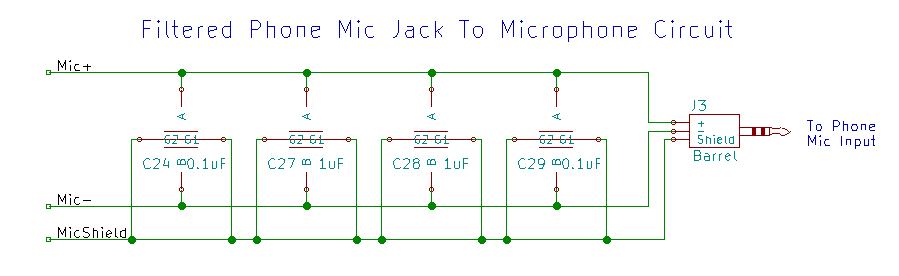
\includegraphics[width=0.7\textwidth]{X2Yfiltercircuit}
	\caption{Pass Through Microphone Filter Circuit}
	\label{fig:x2y}
\end{figure}

In addition, a heatsink will be attached to a large ground plane on one side of the board, and the phone will be attached to the same ground plane, to provide some shielding.

\subsubsection{Enclosure}

A new prototype enclosure is not a hard requirement, but is an essential part of prototyping the entire device, especially given the changes being made to the components inside the enclosure. The designed enclosure is shown in Figure \ref{fig:enclosurefront} and Figure \ref{fig:enclosureback} below.

\begin{figure}[H]
	\centering
	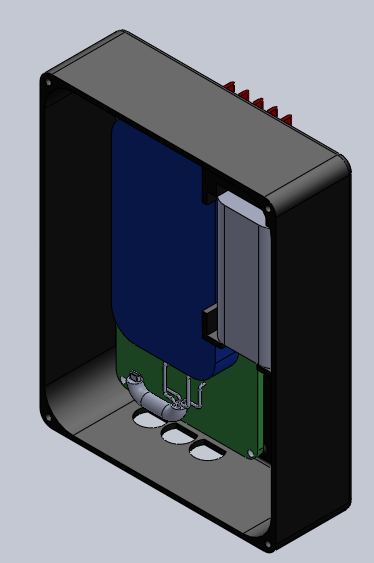
\includegraphics[width=0.8\textwidth]{Assembly2}
	\caption{Front View of the Enclosure}
	\label{fig:enclosurefront}
\end{figure}

\begin{figure}[H]
	\centering
	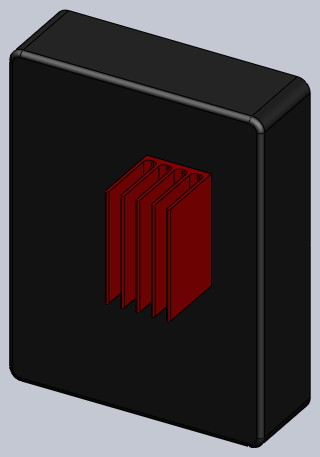
\includegraphics[width=0.8\textwidth]{Assembly3}
	\caption{Back View of the Enclosure}
	\label{fig:enclosureback}
\end{figure}

\subsection{Hardware Implementation} \label{sect:hardwareimp}

\subsubsection{Heatsink} \label{sect:heatsinkimplementation}

A heatsink, as described in Section \ref{sect:heat_just} is shown in Figure \ref{fig:heatsink}.  The current design calls for a rectangular opening to be cut into the front face of the enclosure so that the heatsink may pass through. The opening will be sealed with foam or rubber insulation.

\begin{figure}[H]
	\centering
	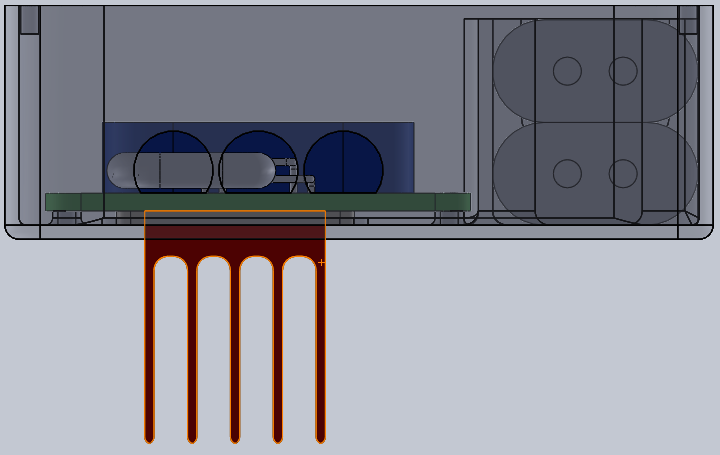
\includegraphics[width=0.8\textwidth]{Assembly4}
	\caption{Heatsink attached to PCB and protruding through the enclosure}
	\label{fig:heatsink}
\end{figure}

The open source thermal simulation tool \textit{Energy 2D} was used to simulate the benefits of a heatsink. The following image (Figure \ref{fig:thermal}) shows a simulation with an ambient temperature of 30$^{\circ}C$ and the phone (the white rectangle) starting at 125$^{\circ}C$ and dissipating into the enclosure (the grey box). In the simulation, the red areas are at around 30-40$^{\circ}C$ while the white areas are significantly hotter, at around 100-125$^{\circ}C$. The enclosure has the thermal properties of ABS plastic, while the heatsink has the thermal properties of aluminum. The simulation shows the heatsink dissipating heat outside of the enclosure, reducing the overall heat inside.

\begin{figure}[H]
	\centering
	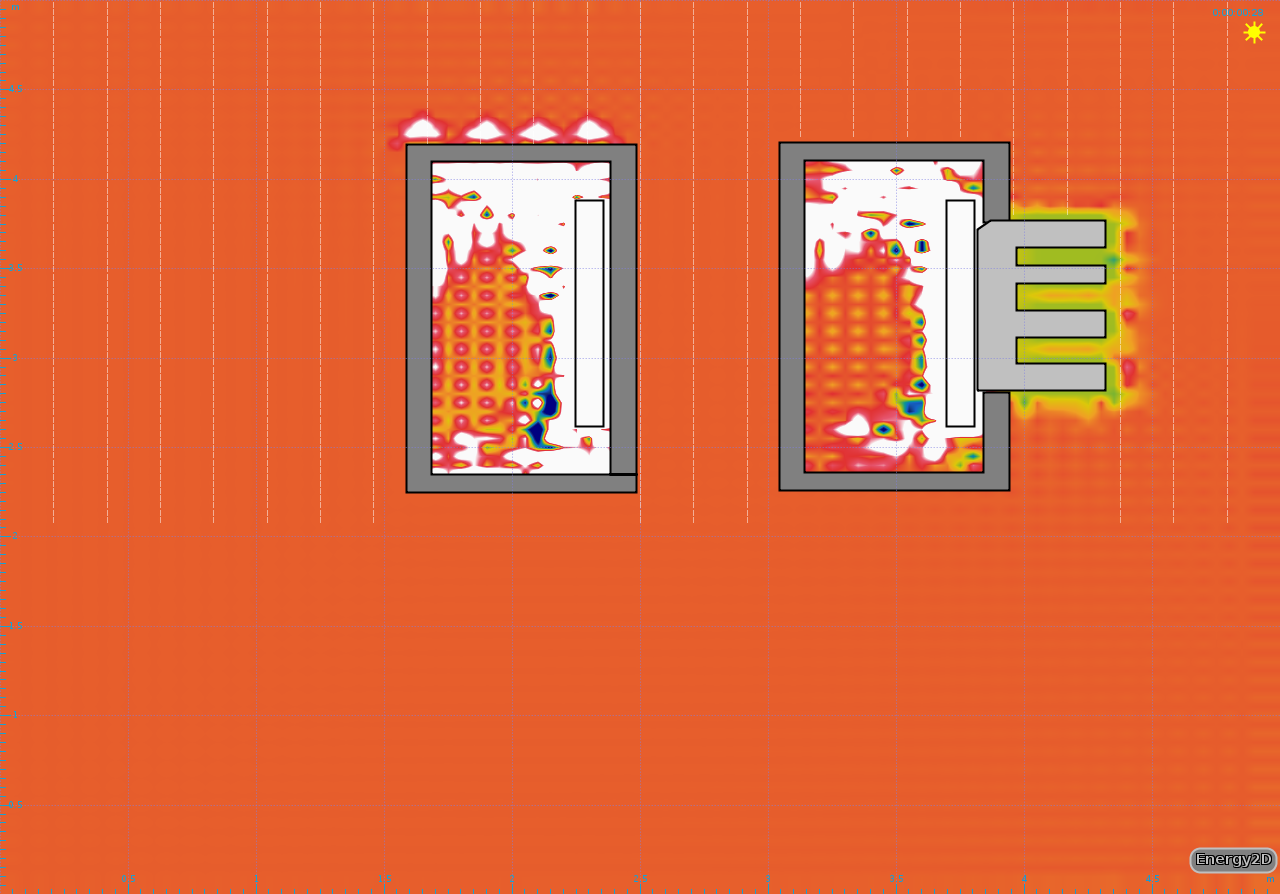
\includegraphics[width=0.8\textwidth]{thermal4}
	\caption{An Energy 2D simulation: On the left: Phone in enclosure with no heatsink. On the right: Phone in enclosure and attached to heatsink}
	\label{fig:thermal}
\end{figure}

\newpage
\subsection{Software Design} \label{sect:softwaredes}
The software used in the design will consists of C and C++ code running on the ATMega328P microcontroller, as well as a companion app (RFCx Sentinel) written in Java, running on the Android phone.
\begin{figure}[H]
	\centering
	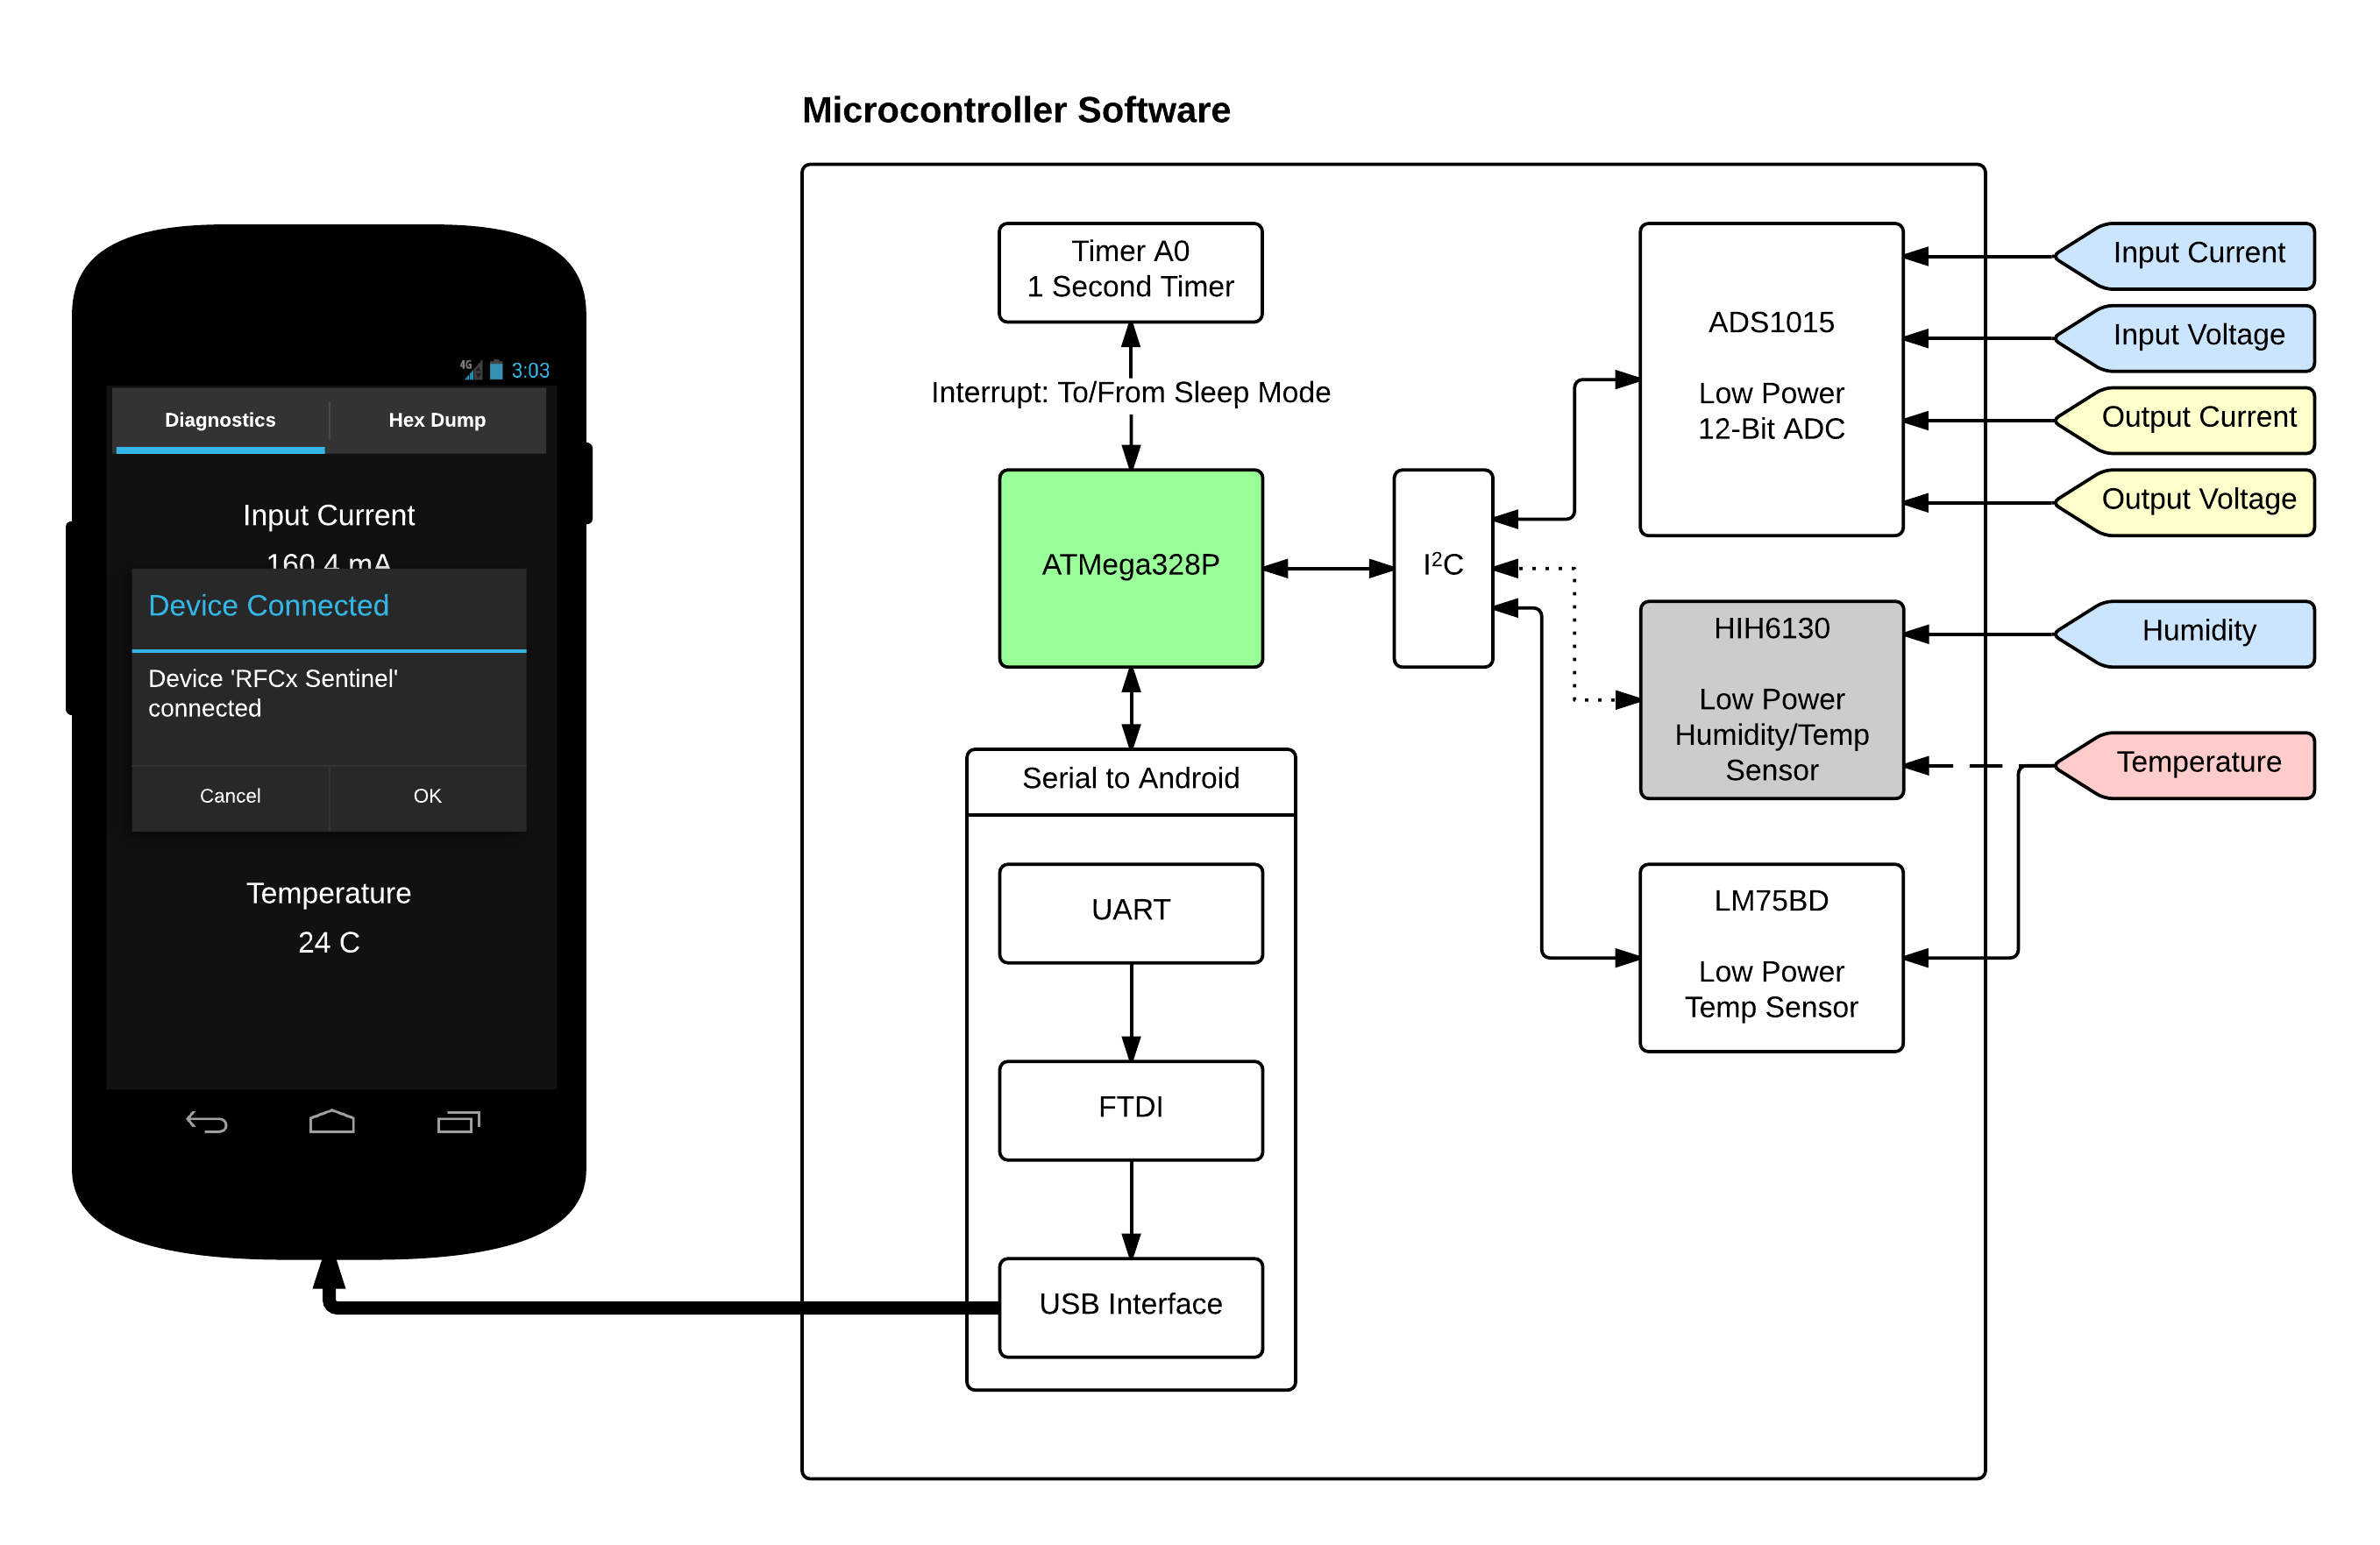
\includegraphics[width=0.8\textwidth]{SoftwareUMLV2}
	\caption{Software UML Diagram}
	\label{fig:swuml}
\end{figure}

The microcontroller software gathers data from a humidity/temperature sensor, and input/output current and voltage. This data is sent via the ATMega328P serial port to the Android phone via the FTDI chip on the PCB and the usb-serial-for-android libraries on the phone.
Listing \ref{lst:snip} describes the basic functionality of the microcontroller software.

\begin{lstlisting}[language=C,label=lst:snip,caption=MCU Flow Code Snippet]
void wakeFromSleep() {
    //Get sensor measurements
    GetDiagnostics(&Diagnostics);
    //Send sensor measurements to phone
    SendDiagnostics(Diagnostics);
    //Go to sleep
    enterSleep();
}
\end{lstlisting}

\subsection{Software Implementation} \label{sect:softwareimp}

An ATMega328P microcontroller will be used to take measurements from the sensors. The temperature (and possibly humidity) measurements are sent digitally via $I^2 C$ to the microcontroller. On the same $I^2 C$ bus is the ADS1015, which has four single-ended analog inputs for reading the input current, input voltage, output current, and output voltage. This data will be sent to the phone using the standard AVR UART serial library.

The data, once sent to the phone, will be monitored by the RFCx Sentinel app. This app is written in Java in Android Studio, and uses the open-source usb-serial-for-android library. The app opens a connection upon discovering a compatible device (FTDI is compatible), and allows the user to view a streamlined interface with relevant data, as well as a tab for the raw hex dump of incoming serial data.

\section{Verification} \label{sect:verification}
This section outlines the steps that are planned to verify that the hardware and software operate in the intended manner.
\subsection{Hardware Verification} \label{sect:hardwareverification}
To verify the power consumption of the devices in \ref{HWa}. the voltage applied and current drawn by the both the enhanced device and the current device will be measured over the course of 1 hour during a realistic usage scenario. The average power will be verified to not exceed 90\% of the existing device’s usage.

To verify \ref{HWf}. a visual inspection by volunteers will qualify camouflage schemes. A successful inspection will be one in which more than 80\% of the volunteers are unable to find the device within a 2 minute inspection window.

To verify \ref{HWg}. a sample group of people with varying skill levels will be asked to provide feedback the on assembly process.

\subsection{Software Verification} \label{sect:softwareverification}
To verify \ref{SWa}., audio will be recorded and compressed using multiple algorithms including the current algorithm. An infographic hosted on RFCx’s website, shown in Figure 2 illustrates the flow of data that is collected from the phone and analyzed on the server.

To verify \ref{HW3}, simple packets will be sent from the microcontroller to the phone. These packets can be verified with debug tools or simple programs on the microcontroller and the phone. A debug serial port may be included as a peripheral to the microcontroller to aid in debugging. Any analog values read by the microcontroller will be verified with shop equipment.

\section{Validation} \label{sect:validation}
\ref{HW3}, \ref{HWb}, and \ref{HWd} can be validated by inspecting the components on the PCB to ensure all required components are present on the board. Requirements \ref{HWg} and \ref{HWh} can be validated by handing the assembly instructions out to a sample group of people with varying skill levels and receiving feedback on the set of instructions from them. People with the ability to read other languages can be used if the documents have been translated from English into other languages.

\ref{HW4} can be validated by inspecting the total cost printed on the BOM for the enhanced device.

\ref{HW1}, \ref{HWa}, and \ref{HW3} can be validated by current and voltage measurements taken in the lab using a DMM. The power calculations made based on those measurements can be compared to similar calculations based on measurements taken from the current device. SPICE simulation data and values displayed on the RFCx Sentinel app will be compared to the actual power consumption of the new device.

\ref{SW1}, \ref{SW2}, \ref{SW3}, and \ref{HW3} can be validated by comparing the values reported in the RFCx Sentinel app to the calculated power consumption of the enhanced device.

\ref{HWc} can be validated by changing the scale factor in the microcontroller program, reprogramming the microcontroller from the PCB header and comparing the values displayed on the RFCx Sentinel app to the previous displayed values. The new values displayed on the RFCx Sentinel app should reflect the change to the scale factor in the microcontroller program.

\ref{HWc}, \ref{SW3}, and \ref{SWa} can be validated during a field test. The enhance device can be mounted at eye level in a tree and turned on to allow the device to start sending audio data to the RFCx server. Requirement \ref{HWf} can be validated by having a volunteer outside of the project search for the device in a wooded area without knowing what it looks like to see if it sticks out. A chainsaw can be turned on 0.25 miles from the device to trigger an alert and validate that the enhanced device can communicate with the RFCx server. The size of the audio recording sent to the RFCx server after employing the audio compression algorithm can be compared to the size of audio data sent to the RFCx server by the current device to determine the audio compression ratio of this algorithm. Both audio recordings can be played back to determine the level of audio interference created by GSM transmission.

\section{Conclusion}\label{conclusion}
This section describes the conclusion of the project including modifications performed on the hardware and software sides. These modifications include two revisions of the PCB, substantial additions to the microcontroller software, and changes to the enclosure, panel frame, and mounting hardware.

\subsection{PCB Modifications}
\subsubsection{1st Revision}\label{conclusion-pcb-rev1}
\paragraph{Design}
The first revision of the board was designed for a specific case in mind and was monolithic. A 3D rendering of the board can be seen in figure \ref{fig:b1}
\begin{figure}[H]
	\centering
	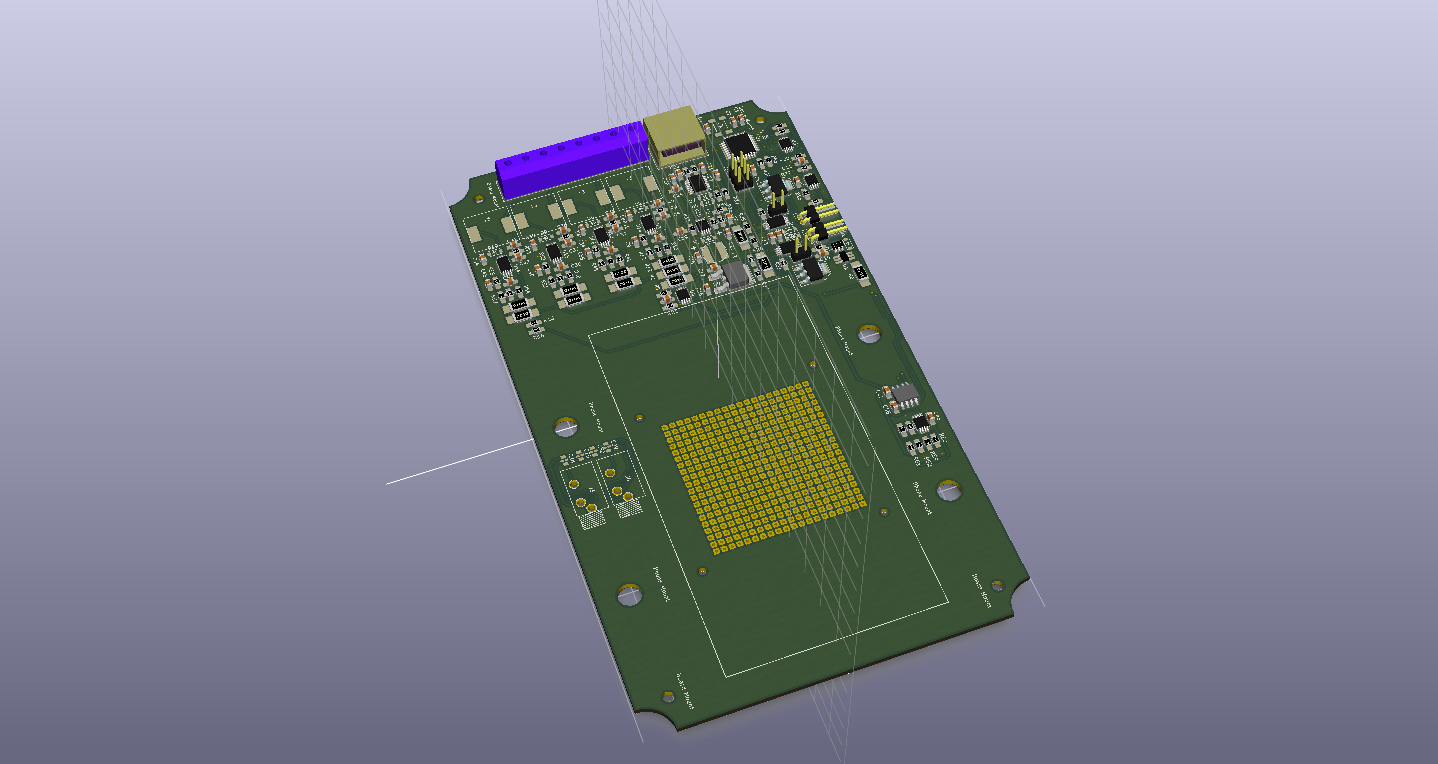
\includegraphics[width=0.8\textwidth]{RFCxrev1_top}
	\caption{First revision of PCB design}
	\label{fig:b1}
\end{figure}

\paragraph{Issues}
Several issues became apparent during assembly and construction of this revision of the design.
\begin{itemize}
\item Monolithic design meant that a problem on the board could render the whole board useless
\item Position of certain components interfered physically
\item An external pullup resistor on the RESET pin of the microcontroller was mistakenly omitted.
\item Footprint for the HIH humidity sensor was too big
\item Thermocouples were not long enough to reach the batteries
\item There was no LED on the ATmega328P to use as a status LED or for debugging
\item The sense resistor between the regulators and the power path management was too small
\item The ADS1015 required a pullup resistor on the ALERT GPIO pin
\item The capacitors on the XTAL were the wrong value, they should be around 6pF
\item The output capacitor of the 3.3V regulator was not connected to GND on the schematic
\end{itemize}
\paragraph{Solutions}
The monolithic board issue was resolved by breaking the board into two separate boards. One board contained the MPPT circuitry and the other board contained the regulation circuitry for the 3.3V and 5V rails, the microcontroller, environment sensors, and the usb interface. This way, the funtionality of the main board can be retained while the power source can be changed. The two boards were made smaller so that they can fit into a multitude of enclosures and be positioned in different ways. Parts that were mistakenly omitted were included for the design of the second revision, and footprints and other issues were corrected.
\subsubsection{2nd Revision}\label{conclusion-pcb-rev2}
\paragraph{Design}
The second revision of the board focused on modularity and compactability so that the enclosures that it fit in are not as constrained as the first revision. A 3D rendering of the second revision of the board can be seen in figure \ref{fig:b21} and \ref{fig:b22}. An LED was also added to the board to aid in rudimentary debugging.

\begin{figure}[H]
	\centering
	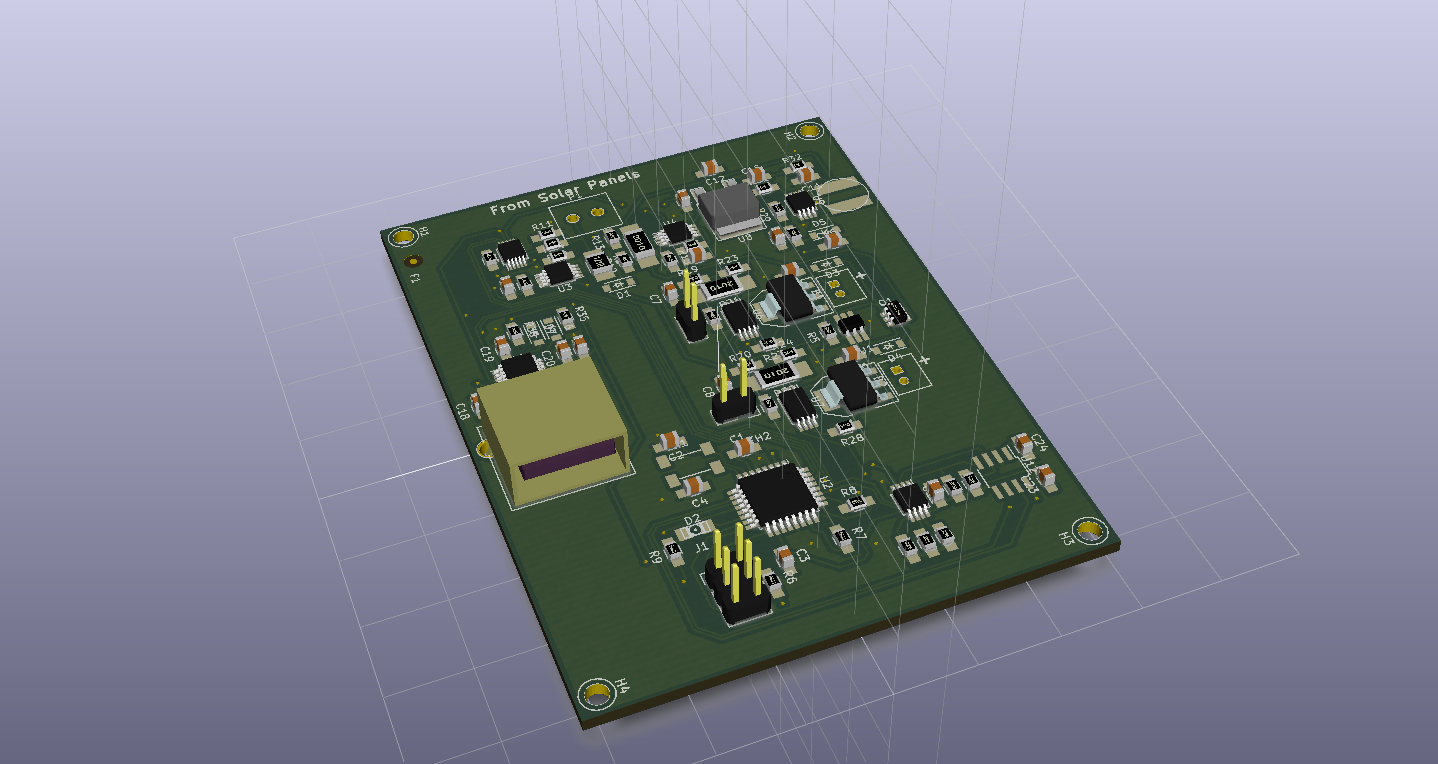
\includegraphics[width=0.8\textwidth]{Mainboard_top}
	\caption{Main Board of Revision 2}
	\label{fig:b21}
\end{figure}

\begin{figure}[H]
	\centering
	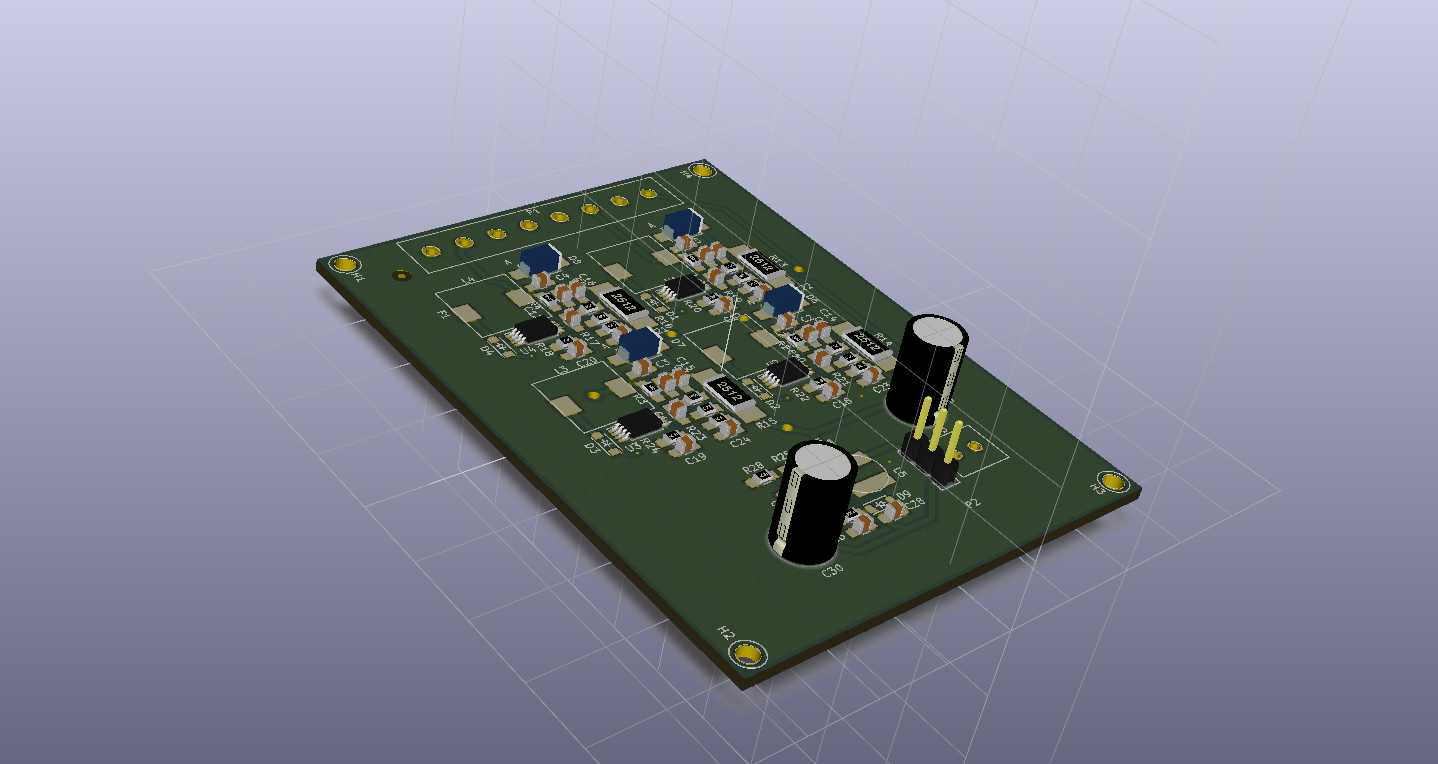
\includegraphics[width=0.8\textwidth]{MPPTboard_top}
	\caption{MPPT Board of Revision 2}
	\label{fig:b22}
\end{figure}

\paragraph{Issues}
The second revision of the board was not without issues. Certain subsystems were difficult to test on the first revision of the board, leading to untested systems moving through to the second revision of the board. Some of the issues include:
\begin{itemize}
\item Swapped D+ and D- signals on the usb Interface
\item FTDI needs a voltage sense divider
\item Footprint on external ADC is wrong, the address pin is unconnected (must be pulled up to VCC)
\item The output capacitor of the 5V regulator was rated at only 6.3V, which is not enough to cover voltage spikes
\item The GSM audio filtering board needs to be printed
\item The X2Y capacitors have a footprint that is very difficult to solder
\item The ICSP silkscreen should include a small tab where the connector has a tab so it is clear how to align it
\item There are +/- signs missing on the silkscreen for the terminal header connectors
\item The battery connector footprints are backwards
\item R1 and R2 (the input/output sense resistors) should use the same footprint
\item The main board terminal header label ``From Solar Panels'' should read ``From MPPT Board''
\item 0$\Omega$ resistors should be used instead of wires to pull up/down the address pins on the LM75BD
\item Some part labels are misleading or covered up by components
\end{itemize}
\paragraph{Solutions}
For a short term fix, the signals that were routed wrong were soldered with wire on the board so that tests could be carried out. For the third revision of the board, these issues will be fixed.
\subsubsection{Future 3rd Revision}\label{conclusion-pcb-rev3}
\paragraph{Design}
The next revision of the board will have the routing fixes that made it to revision 2. This revision of the board design is meant to be a version that can be field tested. All issues descibed in the section for the second revision will be fixed.
\subsection{Software Modifications}\label{conclusion-software}
The software modifications were almost exclusively done to the microcontroller software. The microcontroller software was taken from a very simple piece of code that generated random values and sent them over USART on the Arduino to a functional piece of microcontroller code running on the actual board that can read sensors and transmit them to the phone.
\subsubsection{Microcontroller Software}\label{conclusion-mcu-software}
The microcontroller software underwent substanital changes, and was basically completely rewritten. The code now includes functions to read the temperature from the LM75BD, read the temperature and humidity from the HIH6130, read the input and output voltages and currents from the ADS1015, and read the battery charging status from the BQ2057. The microcontroller code can be found in section \ref{sect:mcu-source}.

\subsection{Enclosure Modifications}\label{conclusion-enclosure}
The enclosure and mounting hardware were also modified. A new enclosure was chosen to be a smaller fit and also to include a weather-sealed rubber gasket on the lid. The new enclosure is shown in \ref{sect:appendixC} under \ref{fig:new_case}. The new assemblies are shown in the same appendix under \ref{fig:append_panel_assembly} and \ref{fig:append_panel_case_assembly}.

\subsection{Results of Verification and Validation}\label{conclusion-vv}

\section{Project Budget and Schedule} \label{sect:budgetandschedule}
\subsection{Budget} \label{sect:budget}
This project will require minor funding for manufacturing and populating the PCB, and the materials to construct a new enclosure, as well as general testing and component costs. As RFCx is a non-profit organization working solely on grant money, this budget is not expected to be covered by them.
\begin{itemize}
\item \$400 = 4 x \$100 for PCB manufacturing
\item \$320 = 4 x \$80 for PCB components
\item \$200 = 1 x \$200 for general needs
\item Estimated Total: \$920
\end{itemize}

RFCx

\begin{landscape}
\subsection{Schedule} \label{sect:schedule}
The schedule in Figure \ref{fig:gantt} is the proposed schedule for all phases of the project. This will be used as a general timeline for guidance throughout the project.

\begin{figure}[H]
  \centering
  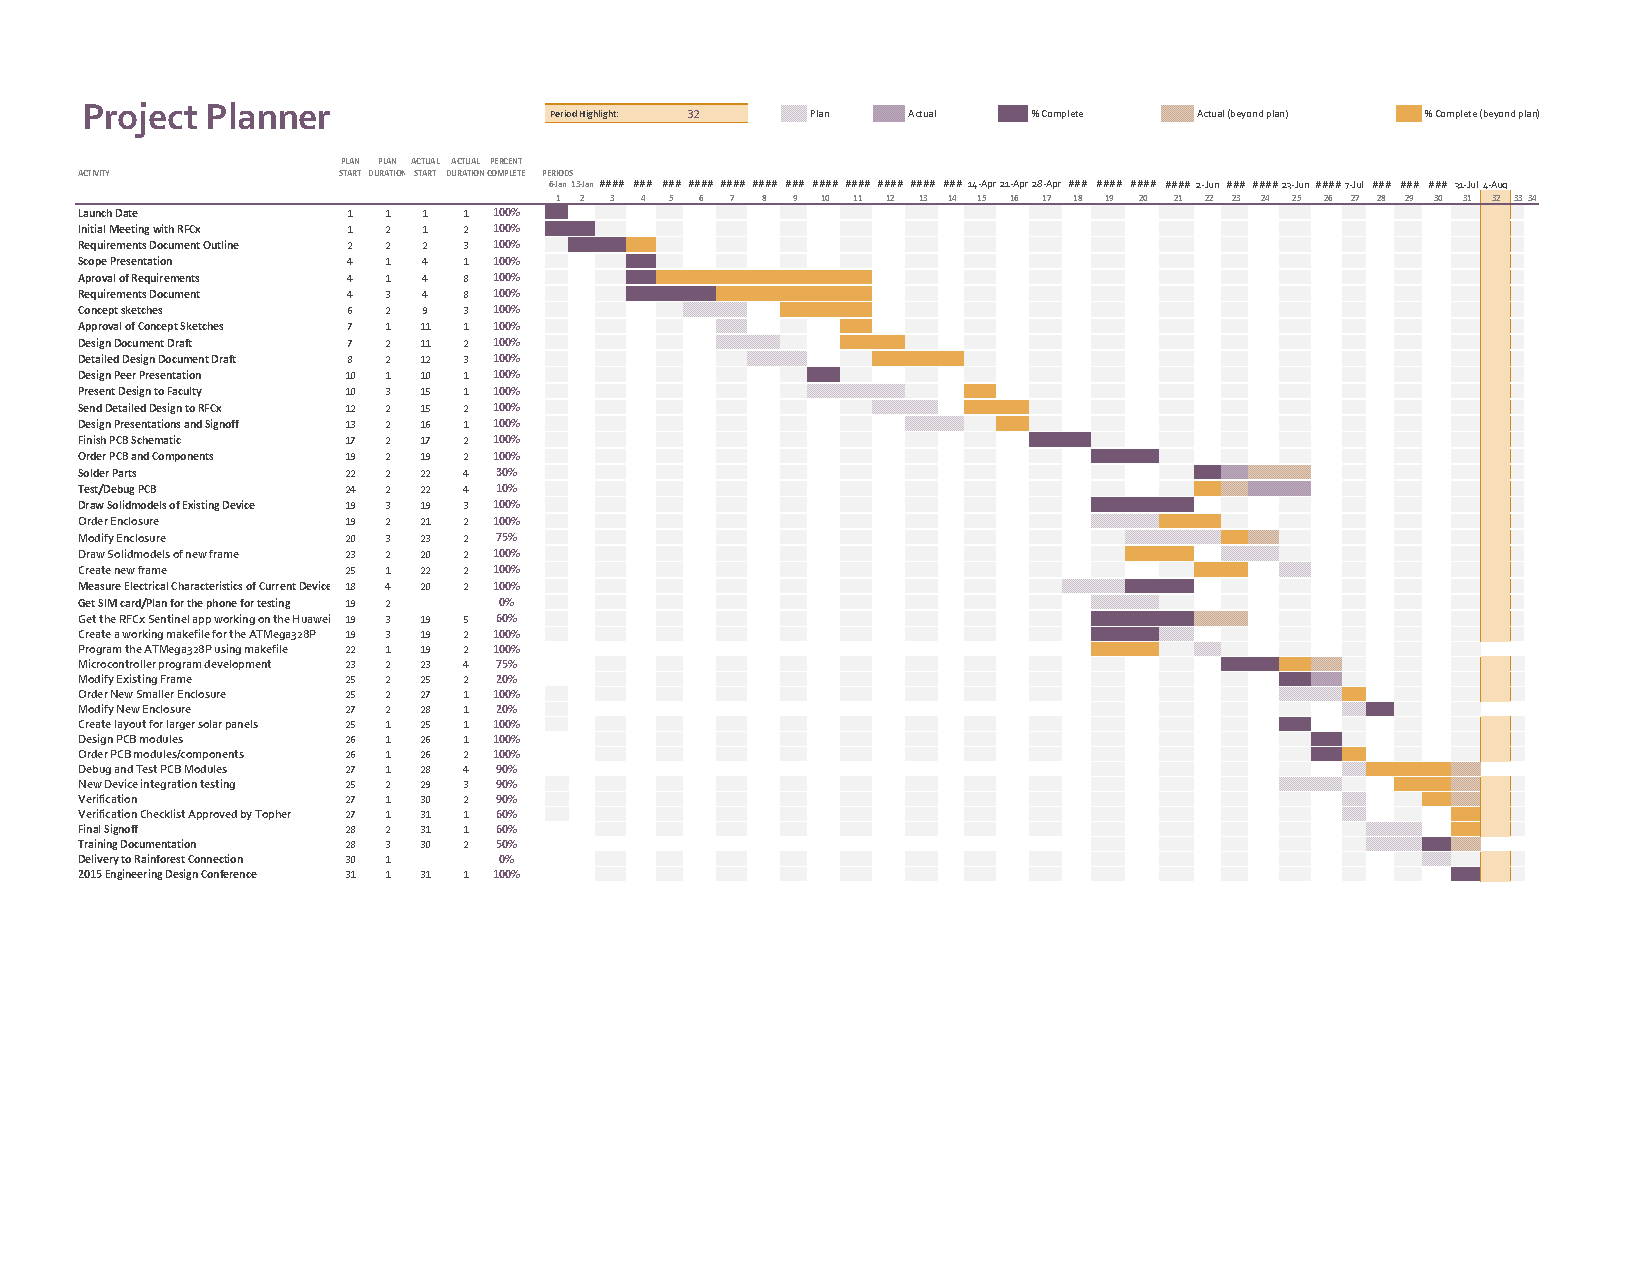
\includegraphics[scale=0.85, trim=0cm 12cm 0cm 0cm, clip=true]{Schedule.pdf}
  \caption{Gantt Chart for Schedule}
  \label{fig:gantt}
\end{figure}
\end{landscape}

\newpage
\section{Sponsor Sign-off}
On behalf of Rainforest Connection(RFCx), the undersigned  approves the functional requirements and design contained in this document that specify the project deliverables and functionality.

\bigskip

\bigskip
\noindent \namesigdate{Topher White} \hfill \namesigdate{Dave Grenell}


\newpage
\vspace*{\fill}
\section*{\centering{Appendices}}
\addcontentsline{toc}{section}{Appendices}
\vspace*{\fill}
\newpage
\appendix
\section{Electrical Schematics and Simulations} \label{sect:appendixA}
% \makeatletter
% \@addtoreset{figure}{section}
% \makeatother
% \renewcommand\thefigure{\current.\arabic{figure}}

\begin{figure}[H]
	\centering
	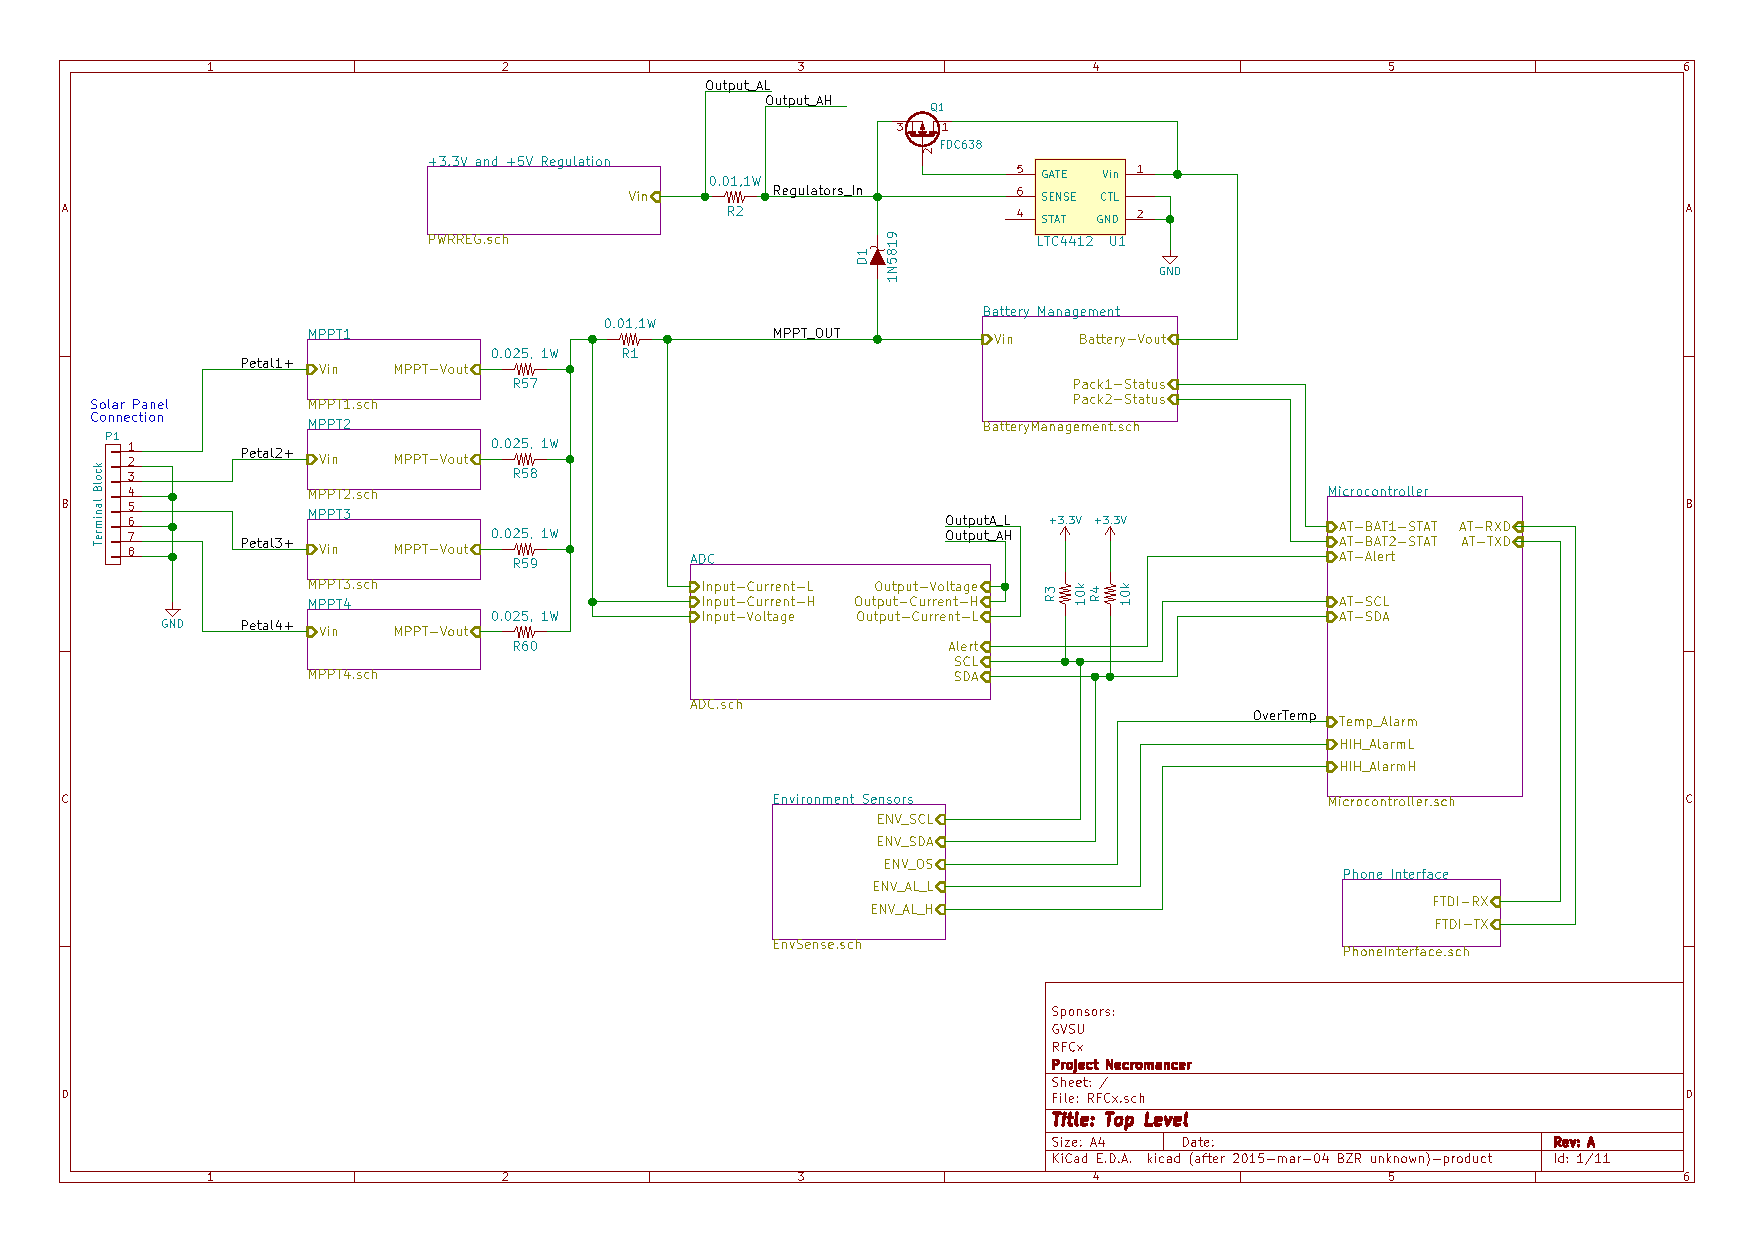
\includegraphics[page=1,width=0.9\textwidth]{RFCxSchematics.pdf}
	\caption{Top Level Schematic}
	\label{fig:schemp1}
\end{figure}

\begin{figure}[H]
	\centering
	\includegraphics[page=2,width=0.9\textwidth]{RFCxSchematics.pdf}
	\caption{ATmega328P Microcontroller}
	\label{fig:schemp2}
\end{figure}

\begin{figure}[H]
	\centering
	\includegraphics[page=3,width=0.9\textwidth]{RFCxSchematics.pdf}
	\caption{SPV1040 Max Point Power Tracker (MPPT)}
	\label{fig:schemp3}
\end{figure}

\begin{figure}[H]
	\centering
	\includegraphics[page=4,width=0.9\textwidth]{RFCxSchematics.pdf}
	\caption{ADS1015 External Analog-to-Digital Converter and Instrumentation Amplifiers}
	\label{fig:schemp4}
\end{figure}

\begin{figure}[H]
	\centering
	\includegraphics[page=5,width=0.9\textwidth]{RFCxSchematics.pdf}
	\caption{BQ2057CTS Battery Management Controllers}
	\label{fig:schemp5}
\end{figure}

\begin{figure}[H]
	\centering
	\includegraphics[page=6,width=0.9\textwidth]{RFCxSchematics.pdf}
	\caption{LMR61428 5V Regulator and SM72442 3.3V Regulator}
	\label{fig:schemp6}
\end{figure}

\begin{figure}[H]
	\centering
	\includegraphics[page=7,width=0.9\textwidth]{RFCxSchematics.pdf}
	\caption{Android Phone Interface: FT230X FTDI Serial to USB and Filtered Microphone Pass-through}
	\label{fig:schemp7}
\end{figure}

%@TODO These are just repeats of the MPPT schematic (since there are four... Either remove them from the RFCxSchematics.pdf document and the temp/humidity sensor will be on page 8, or keep them commented out like they are now.)

% \begin{figure}[H]
% 	\centering
% 	\includegraphics[page=8,width=0.9\textwidth]{RFCxSchematics.pdf}
% 	\caption{MPPT}
% 	\label{fig:schemp8}
% \end{figure}
%
% \begin{figure}[H]
% 	\centering
% 	\includegraphics[page=9,width=0.9\textwidth]{RFCxSchematics.pdf}
% 	\caption{}
% 	\label{fig:schemp9}
% \end{figure}
%
% \begin{figure}[H]
% 	\centering
% 	\includegraphics[page=10,width=0.9\textwidth]{RFCxSchematics.pdf}
% 	\caption{}
% 	\label{fig:schemp10}
% \end{figure}

\begin{figure}[H]
	\centering
	\includegraphics[page=11,width=0.9\textwidth]{RFCxSchematics.pdf}
	\caption{LM75BD Temperature Sensor and HIH6130 Temperature and Humidity Sensor}
	\label{fig:schemp11}
\end{figure}

\newpage
\textbf{Power Path Simulations}

The two different power path management circuits were simulated with LTSpice. The two different circuits can be seen below in Figure \ref{fig:doredsim}. On the left is the FET and diode topology. On the right is the chosen Diode-ORing topology. The same diode and transistor were used in each simulation. A load of 550mA was used because this is more than the calculated worst case current draw from the circuit.

\begin{figure}[H]
	\centering
	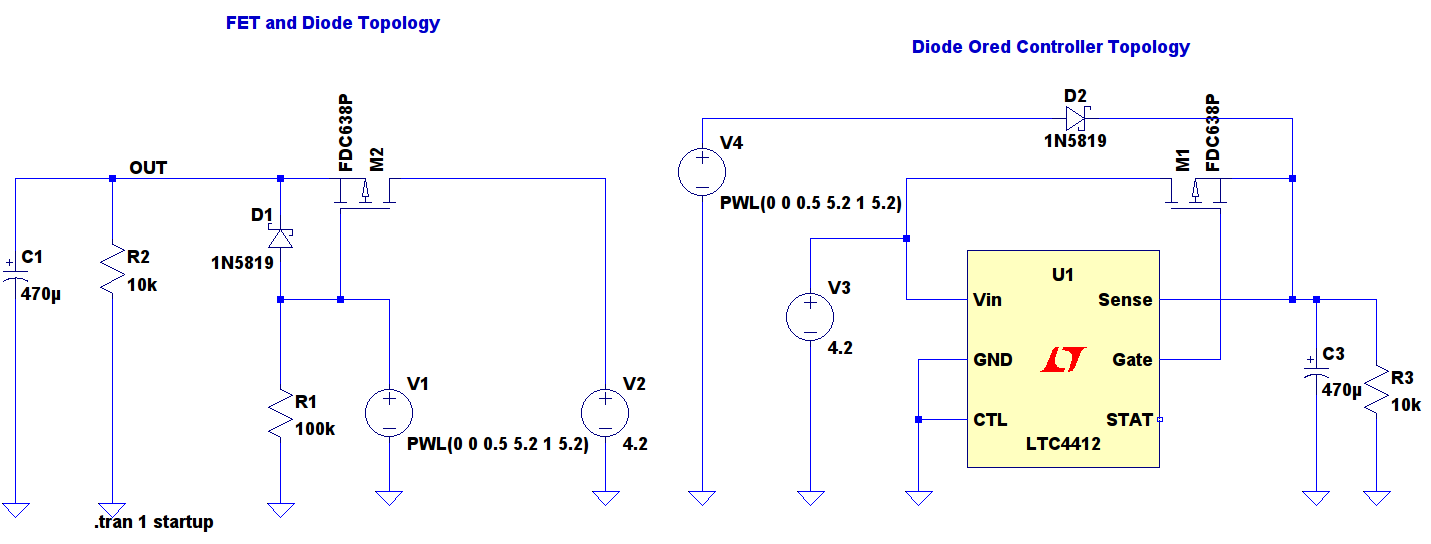
\includegraphics[width=0.8\textwidth]{DiodeORSIM}
	\caption{Two Power Path Management Circuits. Left: FET amd diode topology. Right: Diode-ORed topology}
	\label{fig:doredsim}
\end{figure}

In the simulation for the FET and diode topology, in Figure \ref{fig:doredsimres1}, it can be seen that as the panel voltage is rising, there is a considerable 500mV dip from 3.5V to around 3.0V. If this occured, the 3.3V linear drop out regulator would not be able to regulate properly and the 3.3V line would be deactivated.
\begin{figure}[H]
	\centering
	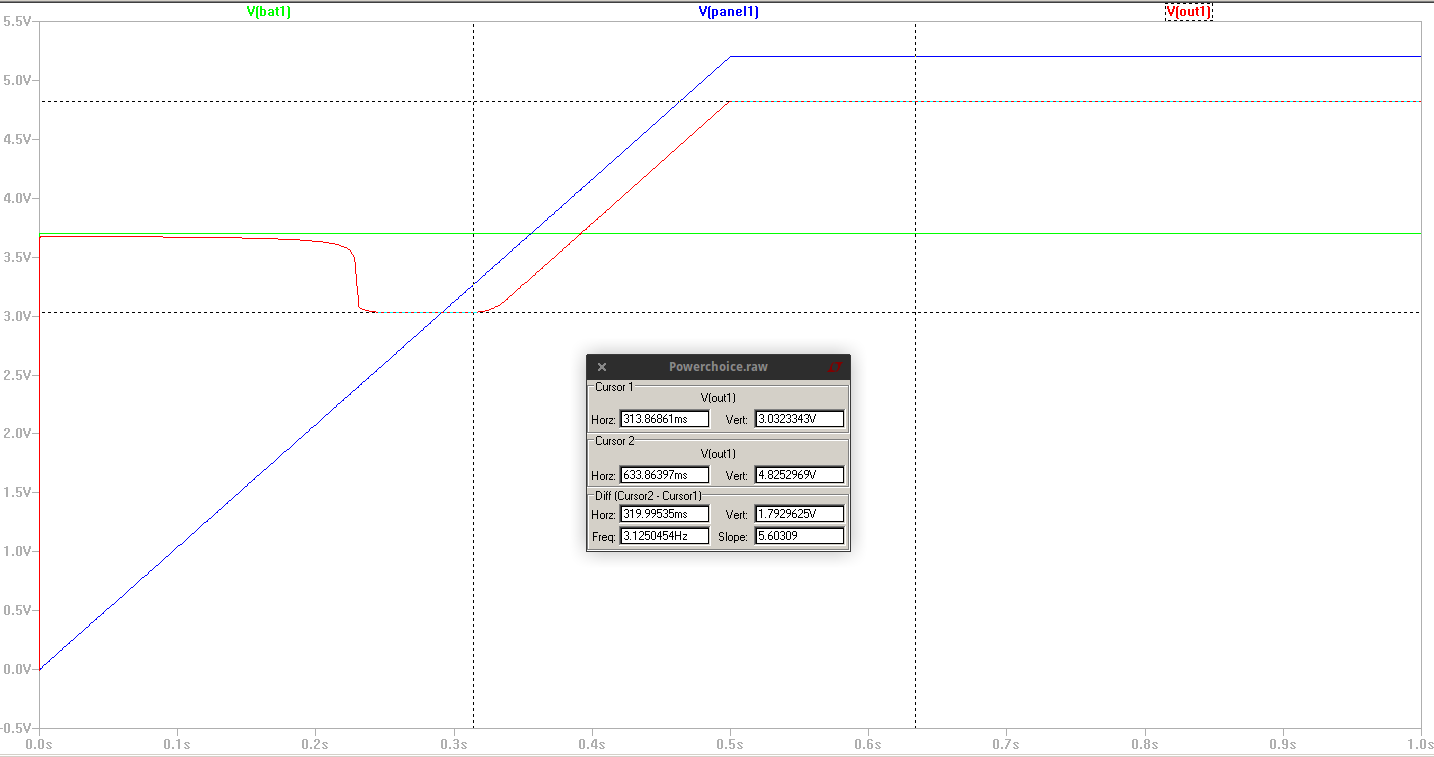
\includegraphics[width=0.6\textwidth]{DiodeORres1}
	\caption{Simulation Result of FET and Diode Topology}
	\label{fig:doredsimres1}
\end{figure}

Conversely, in Figure \ref{fig:doredsimres2} the Diode-ORed topology simulation shows an extremely small drop in voltage when powered from only the batteries and a reasonable drop when powered from the solar panel. This is the desired behavior.
\begin{figure}[H]
	\centering
	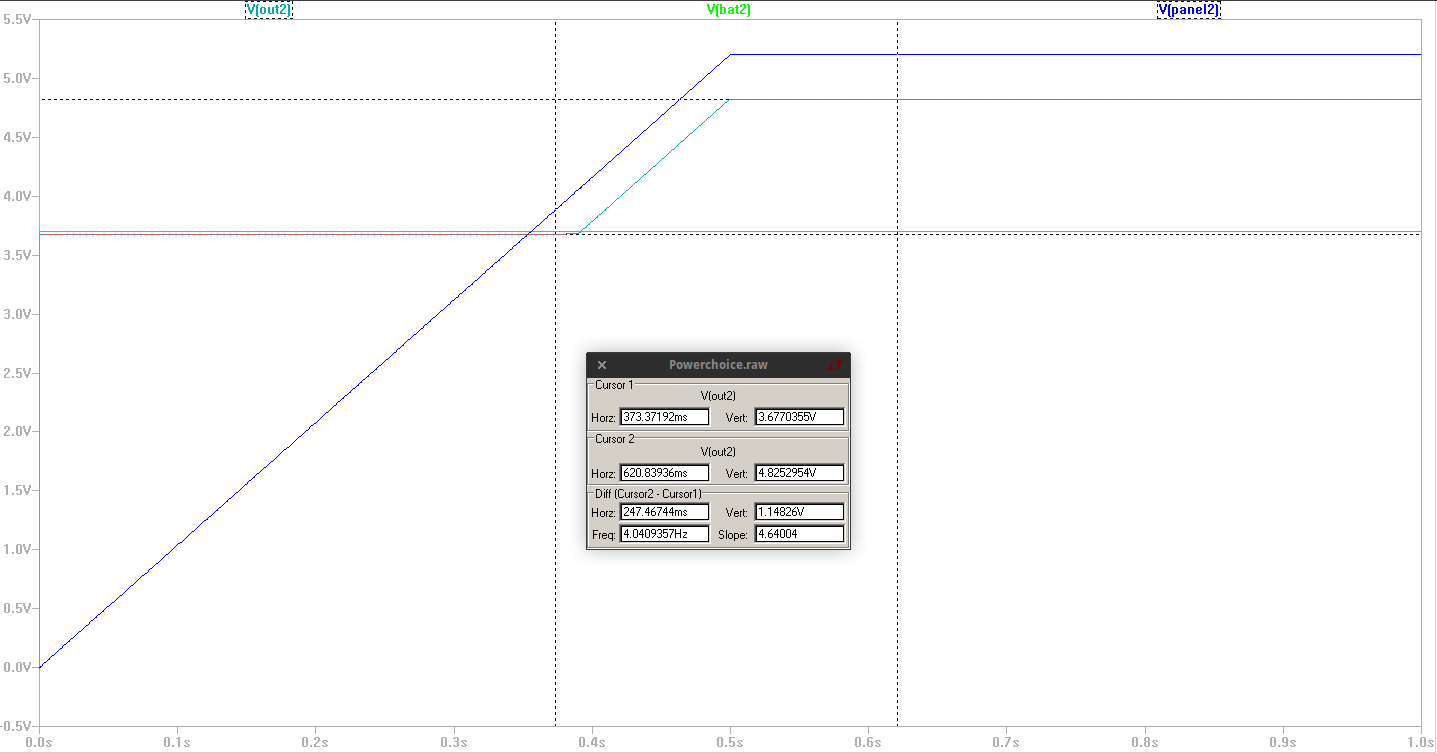
\includegraphics[width=0.8\textwidth]{DiodeORres2}
	\caption{Simulation Result of Current Diode-ORed Topology}
	\label{fig:doredsimres2}
\end{figure}

\newpage
\section{Bill Of Materials} \label{sect:appendixB}
\begin{figure}[H]
	\centering
	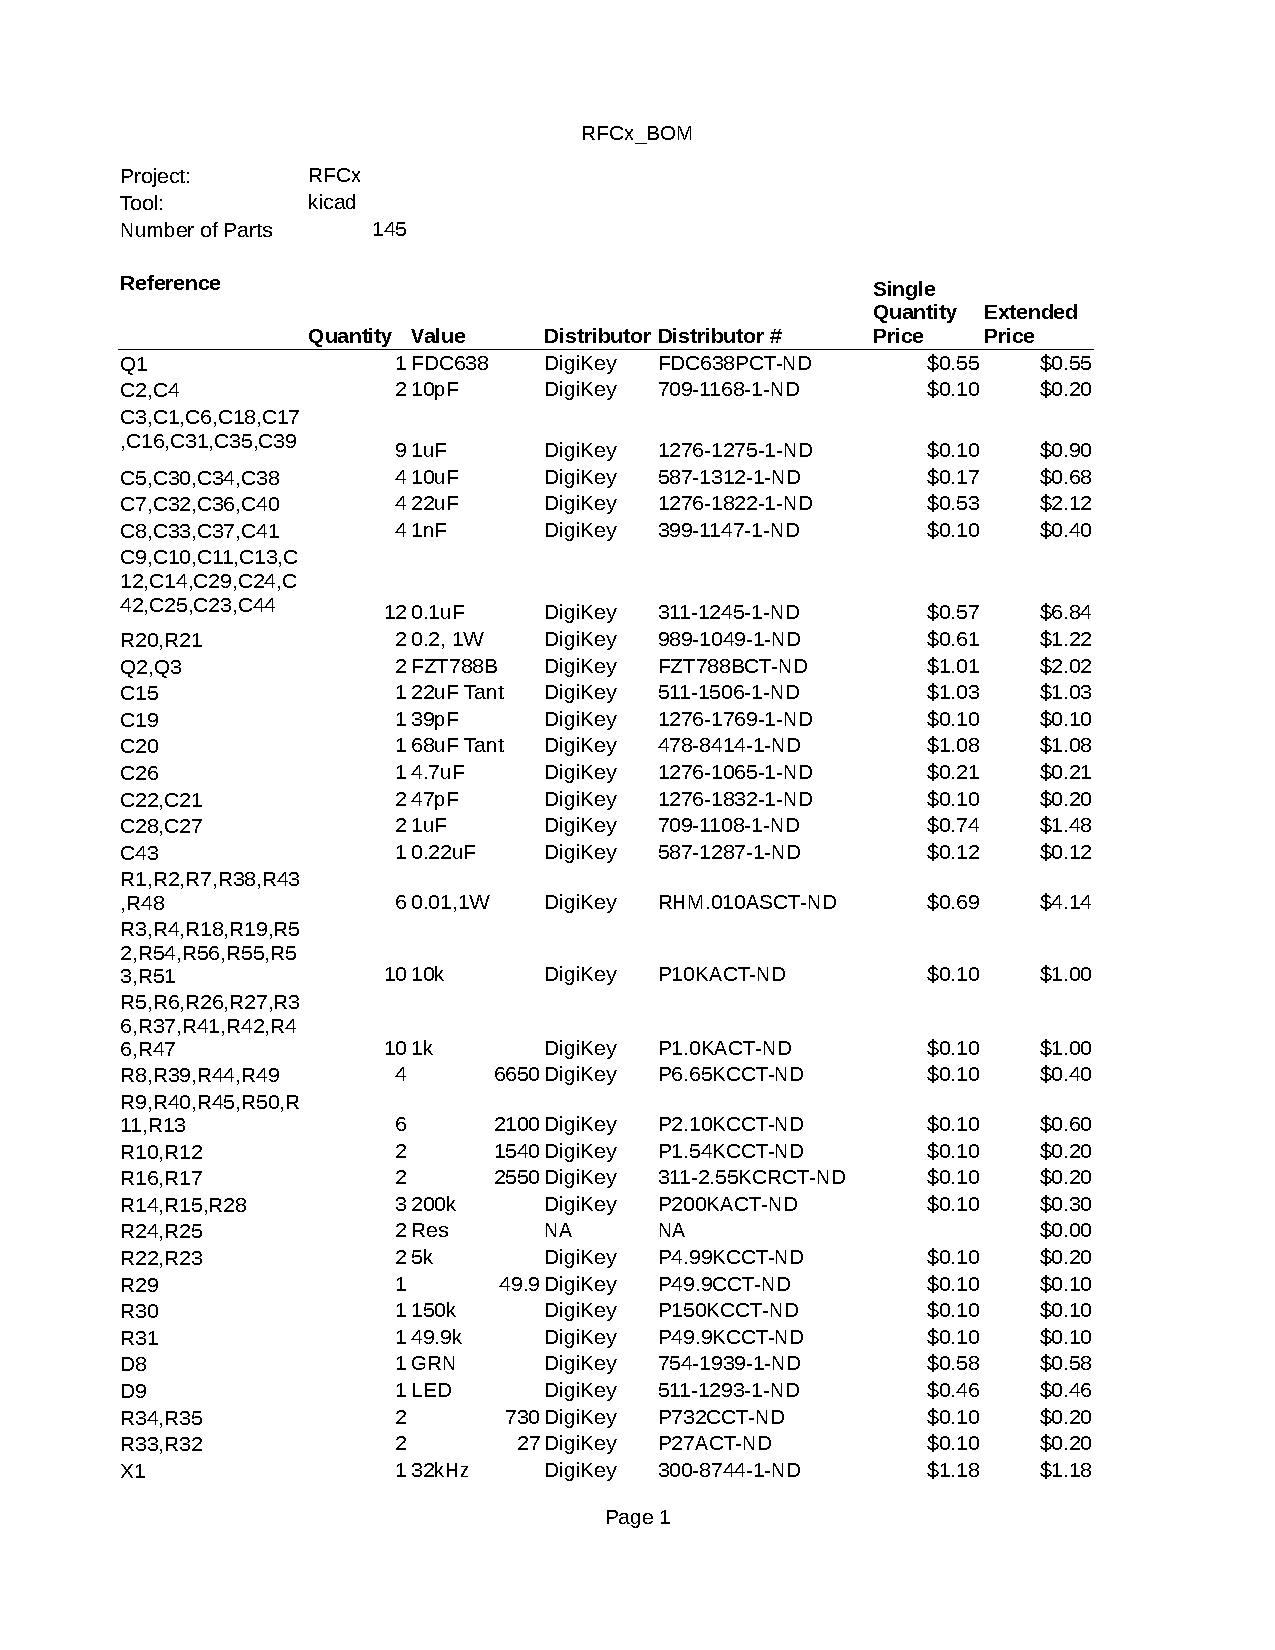
\includegraphics[page=1,width=0.9\textwidth]{RFCx_BOM.pdf}
	\caption{}
	\label{fig:bom1}
\end{figure}
\begin{figure}[H]
	\centering
	\includegraphics[page=2,width=0.9\textwidth]{RFCx_BOM.pdf}
	\caption{}
	\label{fig:bom2}
\end{figure}


\newpage
\section{Mechanical Drawings} \label{sect:appendixC}
\begin{figure}[H]
	\centering
	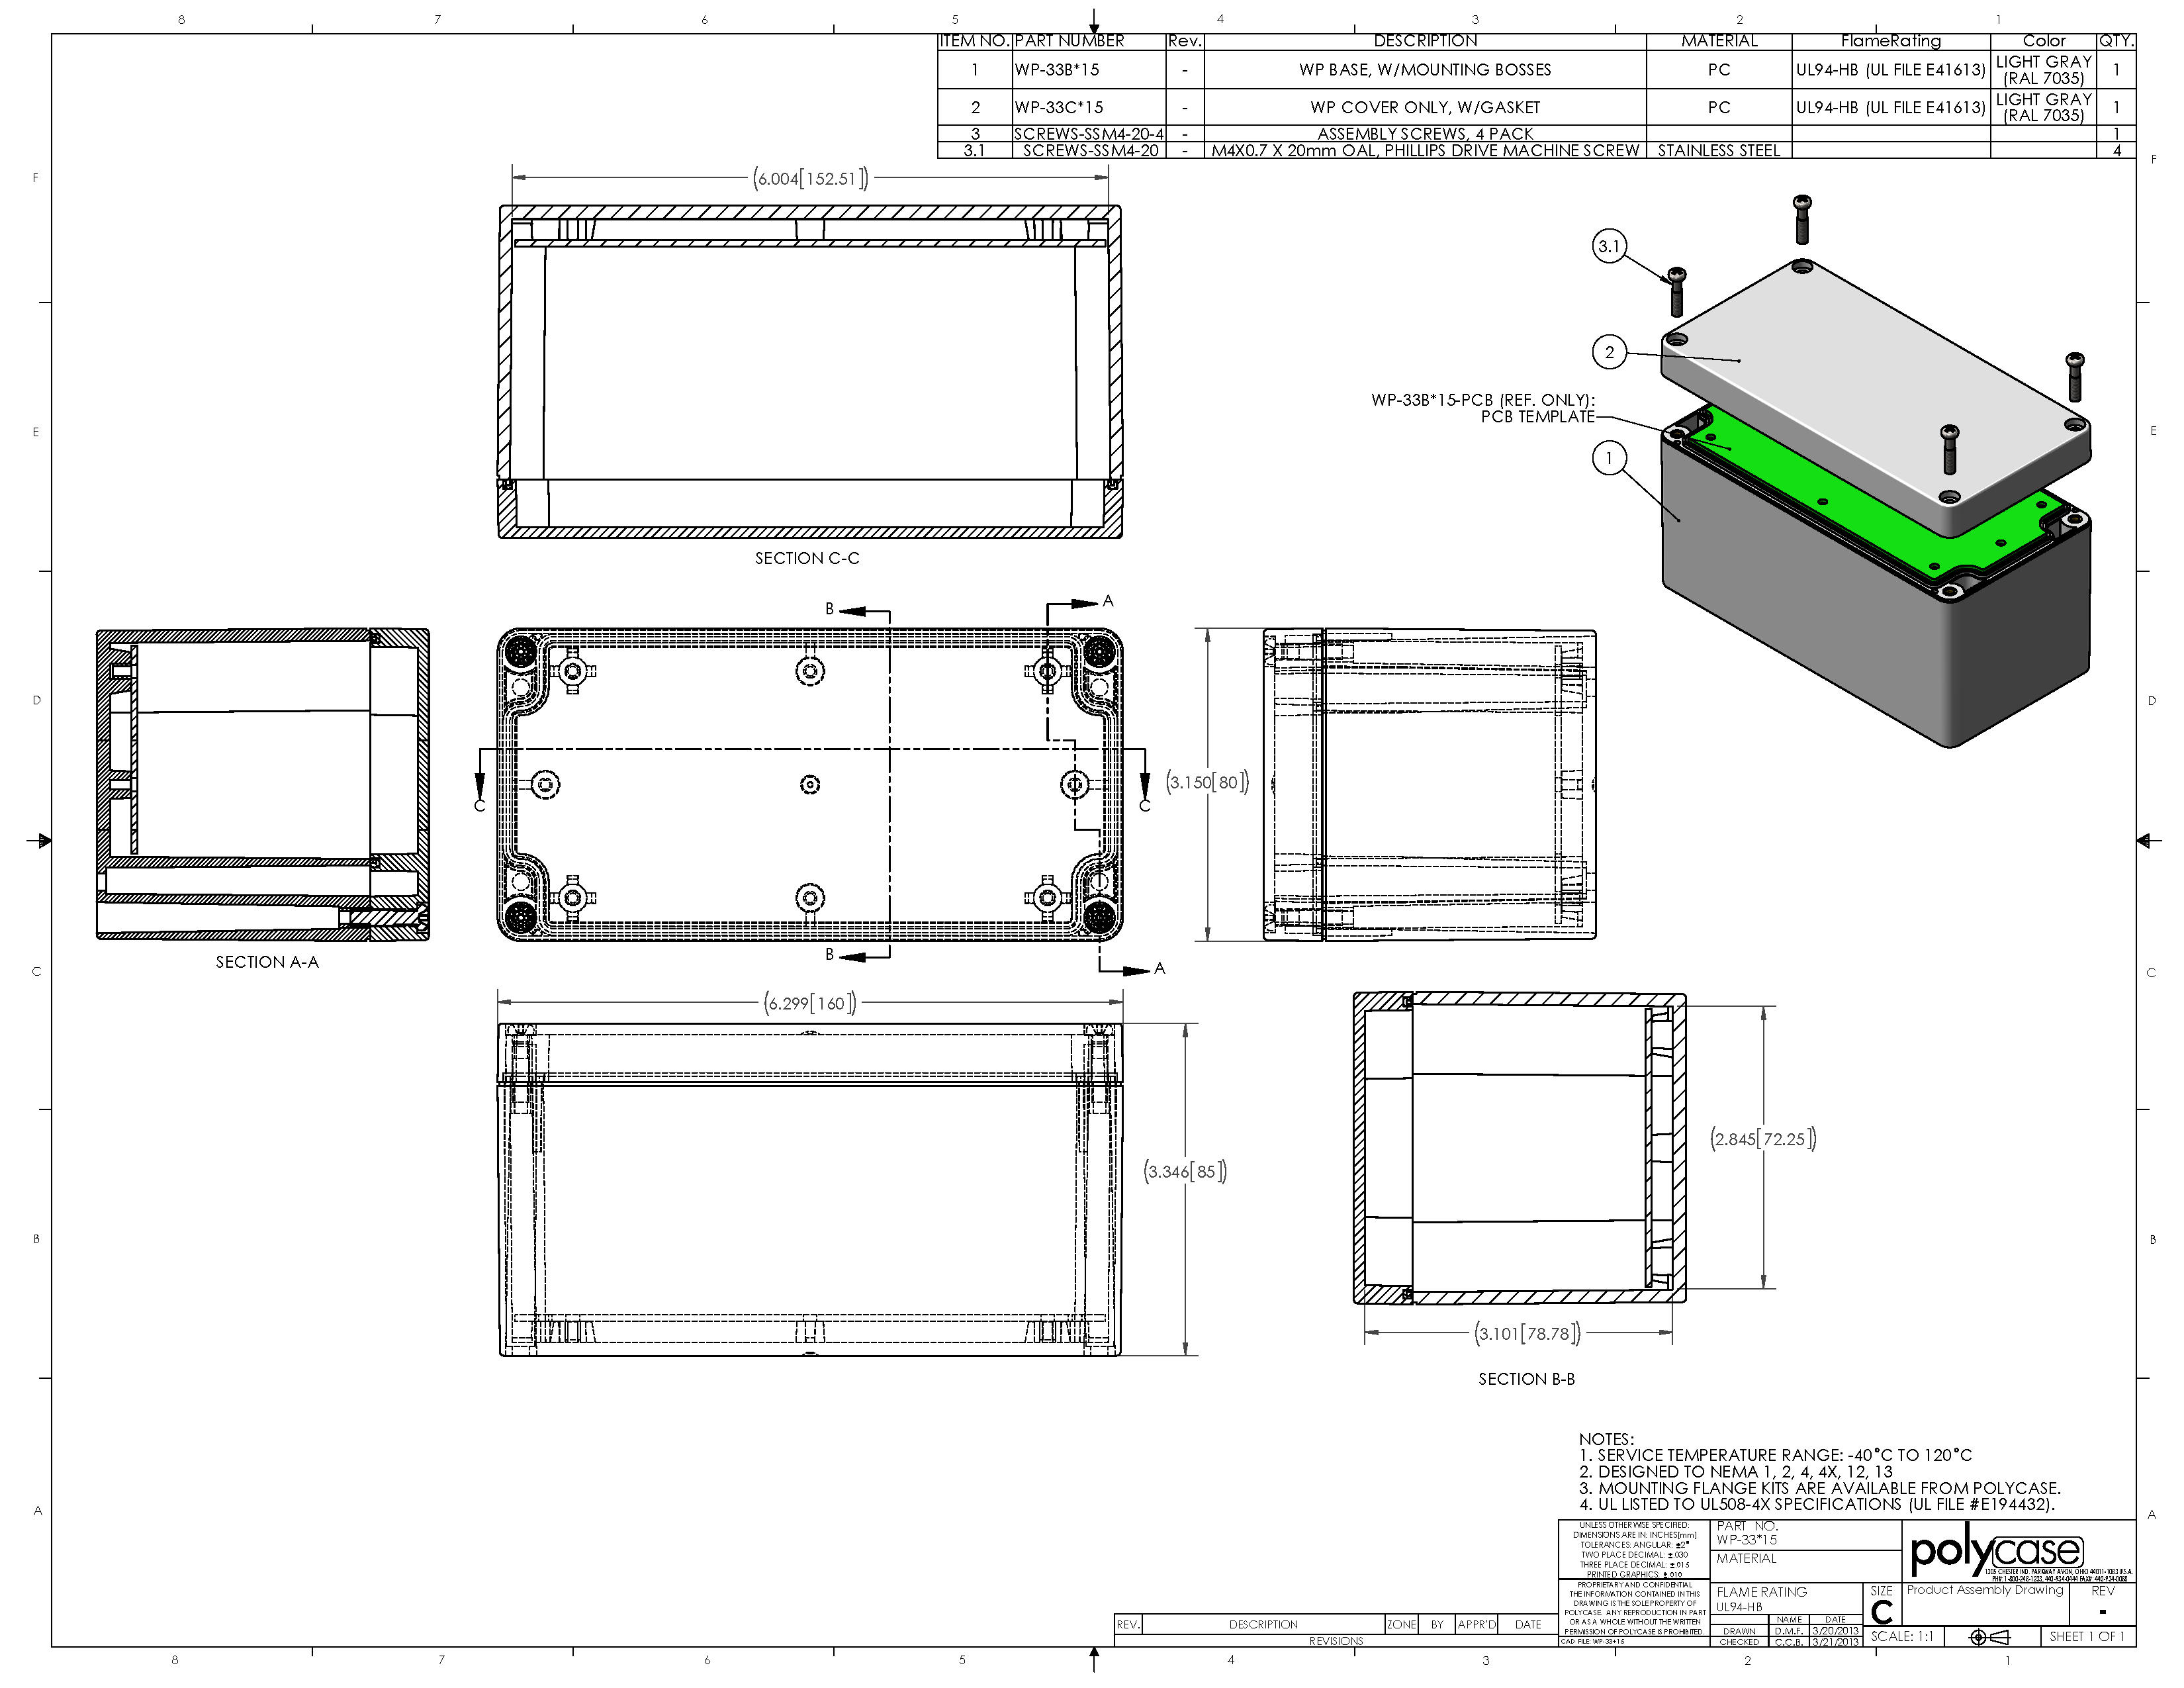
\includegraphics[width=0.8\textwidth]{NewCase.pdf}
	\caption{New Case}
	\label{fig:append_new_case}
\end{figure}

\begin{figure}[H]
	\centering
	\includegraphics[width=0.8\textwidth]{NewAssembly}
	\caption{Panel Assembly}
	\label{fig:append_panel_assembly}
\end{figure}

\begin{figure}[H]
	\centering
	\includegraphics[width=0.8\textwidth]{NewAssembly2}
	\caption{Panel and Case Assembly}
	\label{fig:append_panel_case_assembly}
\end{figure}

\begin{figure}[H]
	\centering
	\includegraphics[width=0.8\textwidth]{PCB}
	\caption{PCB Dimensions}
	\label{fig:append_pcbdimensions}
\end{figure}

\begin{figure}[H]
	\centering
	\includegraphics[width=0.8\textwidth]{PhoneAndPCB}
	\caption{PCB Dimensions}
	\label{fig:append_pcbphone}
\end{figure}

\begin{figure}[H]
	\centering
	\includegraphics[width=0.8\textwidth]{Assembly1}
	\caption{USB Micro A Connector attached to the PCB with strain relief: A small flexible cable}
	\label{fig:append_usbcable}
\end{figure}

\begin{figure}[H]
	\centering
	\includegraphics[width=0.8\textwidth]{Assembly2}
	\caption{Front View of the Enclosure}
	\label{fig:append_enclosurefront}
\end{figure}

\begin{figure}[H]
	\centering
	\includegraphics[width=0.8\textwidth]{Assembly3}
	\caption{Back View of the Enclosure}
	\label{fig:append_enclosureback}
\end{figure}

\begin{figure}[H]
	\centering
	\includegraphics[width=0.8\textwidth]{Assembly4}
	\caption{Heatsink attached to PCB and protruding through the enclosure}
	\label{fig:append_heatsink}
\end{figure}

\begin{figure}[H]
	\centering
	\includegraphics[width=0.8\textwidth]{thermal4}
	\caption{An Energy 2D simulation: On the left: Phone in enclosure with no heatsink. On the right: Phone in enclosure and attached to heatsink}
	\label{fig:append_thermal}
\end{figure}

\newpage
\section{Calculations} \label{sect:appendixD}
\subsection{bq2057CTS Battery Management Calculations} \label{sect:bqcalcs}
\textbf{Current Regulation}
\begin{align}
  \label{eq:currentreg}
  R_{SNS} &= \frac{V_{SNS}}{IO_{REG}} \\
  &= \frac{105mV}{0.2 \cdot 4400mAHr} \\
  &= 119m\Omega
\end{align}
\textbf{Voltage Regulation}
\begin{align}
  \label{eq:voltreg}
  \frac{R_{B1}}{R_{B2}} &= \left(N \cdot \frac{V_{CELL}}{V_{OREG}}\right) - 1
\end{align}

\textbf{Temperature Monitoring} \newline
Using PTC thermistor

\textbf{External PNP Transistor} \newline
Max Power disipation when battery is lowest (3V)
\begin{align*}
  V_{in} &= 5.2 \\
  I_{REG} &= 880mA \\
  V_{CS} &= 0.176 \\
  V_D &= 0.3
\end{align*}
\begin{align}
  \label{eq:diodepwr}
  P_D &= \left(\left(V_{in} - V_D - V_{CS}\right) - V_{BAT}\right) * I_{REG} \\
  &= \left(5.2 - 0.3 - 0.176 - 3\right) \cdot 0.88 \\
  &= 1.517 W
\end{align}
\textbf{Calculate $\beta_{min}$}
\begin{align}
  \label{eq:betamin}
  \beta_{min} &= \frac{I_{Cmax}}{I_{B}} \\
  &= \frac{0.88}{0.035} \\
  &= 25.14
\end{align}
\textbf{Input Capacitor} \newline
$0.1\mu F$ Ceramic recommended on Vcc and Vss pins

\textbf{Automatic Charge Rate Compensation}
\begin{align}
  \label{eq:comp}
  V(z) &= 0.154 \\
  V(comp) &= \frac{0.154}{2.2} \\
  &= 0.07
\end{align}
\begin{align}
  \label{eq:comp2}
  V(pack) &= 4.2 + (2.2 \cdot 0.07)\\
  &= 4.354
\end{align}
\begin{align}
  \label{eq:comp3}
  \frac{V_{comp}}{V_{sns}} &= \frac{R_{comp2}}{R_{comp1}+R_{comp2}}
\end{align}
The data sheet recommended that $R_{comp2}$ be $10k\Omega$ and that $V_{sns}$ be $105mV$
\begin{align}
  \label{eq:rcomps}
  R_{comp1}&=\frac{R_{comp2} \cdot \left(V_{sns}-V_{comp}\right)}{V_{comp}} \\
  R_{comp1}&=\frac{10k \cdot (0.105 - 0.07)}{0.07} \\
  R_{comp1}&=5k\Omega
\end{align}

\textbf{NTC Calculations}
The BC2384-ND $47k\Omega$ NTC Thermistor was used
$RT_2$ was calculated because only the upper bound is of interest
The upper bound temperature was set to $50^{\circ}C$
\begin{align}
  \label{eq:ntc}
  R_{TH} &= 18k\Omega \mbox{ (Property of the NTC)}\\
  R_{TC} &= 673k\Omega \mbox{ Property of the NTC)}\\
  R_{T2} &= \frac{5 \cdot R_{TH} \cdot R_{TC}}{(2\cdot R_{TC})-(7\cdot R_{TH})} \\
  &= 49.65k\Omega \\
  &\cong 49.9\Omega
\end{align}


\subsection{Current and Voltage Sensing}\label{app:cvsense}
Using the LTC6800
\textbf{Output Voltage}
\begin{align}
  \label{eq:vout}
  V_{out} &= \left(1+\frac{R_2}{R_1}\right)\cdot V_{in}
\end{align}
\textbf{ADC Resolution 12-bit}
\begin{align}
  \label{eq:adcres}
  \frac{3.3V}{2^{12}} &= 805\mu V
\end{align}

\textbf{Choose gain of LTC6800}
\begin{align}
  \label{eq:asense}
  ADCres &= \frac{805\mu V}{bit} \\
  \mbox{I want 1mA/bit resolution} \\
  1mA &= \frac{805\mu V}{1bit} \cdot \frac{I}{V_{AmpOut}} \\
  V_{AmpOut} &= 3.3V \mbox{ (Limited by ADC supplly)} \\
  I &= 4.099 \\
  V_{AmpOut} &= Gain \cdot I \cdot R_{sense} \\
  R_{sense} &= 0.01 \Omega \\
  Gain &= 80.5
\end{align}
\textbf{Choose resistors for gain}
\begin{align}
  \label{eq:gainresistors}
  V_{out} &= \left(1+\frac{R_2}{R_1}\right)\cdot V_{in} + V_{REF} \\
  V_{REF} &= 0V \\
  V_{in} &= 0.04V \\
  V_{out} &= 3.3V \\
  Gain &= 1+\frac{R_2}{R_1} = 80.5
\end{align}
Choose resistors to be $R_2=200k\Omega$ and $R_1=2.55k\Omega$.

\subsection{SPV1040 Calculations}\label{app:spvcalcs}
\textbf{Component Values} \\
These are constraints or known values for the calculations
\begin{align*}
  F_{SW}&=70k-130k,typ:100k \\
  V_{IN_RP_MAX}&=1V \\
  I_{SC} &= 1A \\
  T_{MPP} &= ~1ms \mbox{ (tracking time)} \\
  R_{MPPTset} &= 1k\Omega \\
  I_{MP} &= 0.44A\mbox{ (current at maximum power point)} \\
  I_{SC} &= 0.5A\mbox{ (short circuit current)} \\
  V_{MP} &= 3.0V\mbox{ (Voltage at maximum power point) }\\
  V_{OC} &= 3.4V\mbox{ (Open Circuit voltage)} \\
  V_{out_rp_max} &=  0.01 \mbox{ (Maximum output voltage ripple} \\
  V_{OUT_MAX} &= 5.2V \mbox{ (Desired Maximum output voltage)} \\
  I_{OUT_MAX} &= 1.8V \mbox{ (Limitation of the SPV1040)}
\end{align*}
\textbf{Input Capacitor}
\begin{align}
  \label{eq:incap}
  C_{IN}&\geq \frac{I_{SC}}{F_{SW}\cdot V_{IN_RP_MAX}} \\
  &\geq \frac{1}{70k\cdot 1} \\
  &\geq 14.3\mu F
\end{align}
\textbf{Input Voltage Sensing Capacitor}
\begin{align}
  \label{eq:vincap}
  C_{MPPTset}&\leq T_{MPP} \cdot \frac{1}{R_{MPPTset}} \\
  C_{MPPTset}&\leq 10\mu F
\end{align}
\textbf{Inductor Selection}
\begin{align}
  \label{eq:spvind}
  I_{Lrms} &\cong I_{MP}\leq I_{SC} \\
  I_{peak} &= I_{Lrms} + \frac{9e-6 \cdot V_{MP}}{2\cdot L} \\
  I_{Lpeak} &\leq 1.8 \mbox{ Limitation of SPV1040} \\
  L &\geq \frac{1}{2} \frac{9e-6\cdot V_{MP}}{2-I_{Lrms}} = \frac{1}{2}\frac{9e-6\cdot V_{MP}}{2-I_{MP}}\\
  L&\geq 8.5 \mu H
\end{align}
\textbf{Output Voltage Capacitor}
\begin{align}
  \label{eq:outcap}
  Cout &\geq \frac{I_{SC}}{F_{SW}\cdot V_{out_rp_max}} \\
  Cout &\geq 142\mu F
\end{align}
\textbf{Output Voltage Partitioning}
\begin{align}
  \label{eq:outputvpart}
  \frac{R_{VctrlTOP}}{R_{VctrlBOT}} &= \frac{V_{OUT_MAX}}{1.25}-1 \\
  R_{VctrlTOP} &= 76.8k\Omega \\
  R_{VctrlBOT} &= 24.3k\Omega
\end{align}
\textbf{Output Voltage Sense Capacitor}
\begin{align}
  \label{eq:outsensecap}
  C_{Vctrl} &\cong 10\cdot \frac{1}{F_{SW}}\cdot \frac{1}{R_{VctrlTOP}/R_{VctrlBOT}} \\
  C_{Vctrl} &\cong 45.2 \mu F
\end{align}
\textbf{Output Current sensing filter}
\begin{align}
  \label{eq:currentsense}
  R_{S}&= \frac{50mV}{I_{OUT_MAX}} \\
  R_{S}&= 27m\Omega
\end{align}
\textbf{Schottky Diode} \\
Must satisfy the following:
\begin{align*}
  V_F \leq 5.5-V_{BATT_MAX} \mbox{ and } I_F \geq I_{Lmax}
  V_F \leq 0.8 \mbox{ and } I_F \geq I_{Lmax}
\end{align*}
The \textit{Diodes Incorporated }1N5819HW has a $V_F$ of 450mV and a non repetitive peak current of 25A.

\subsection{LM61428 Calculations} \label{app:lm61calcs}
The values for the components were recommended by the data sheet.
\begin{align*}
  L &= 6.8\mu H \\
  C_{in} &= 22\mu F \\
  C_{out} &= 68\mu F
\end{align*}
The diode was recommended to be a Schottky with $I_f$ higher than the load current, 500mA. The reverse voltage must be higher than the output voltage and it must be able to switch fast.

\newpage
\section{Data Sheet Snippets} \label{sect:appendixE}
This appendix contains the 1st sheet of the data sheets for the parts used in this project.
\begin{figure}[H]
	\centering
	\includegraphics[page=1,width=0.9\textwidth]{combined.pdf}
	\caption{1st Page of ADS1013 Datasheet}
	\label{fig:adsdat}
\end{figure}
\newpage
\begin{figure}[H]
	\centering
	\includegraphics[page=2,width=0.9\textwidth]{combined.pdf}
	\caption{1st Page of ATmega328P Datasheet}
	\label{fig:atmeldat}
\end{figure}

\begin{figure}[H]
	\centering
	\includegraphics[page=3,width=0.9\textwidth]{combined.pdf}
	\caption{1st Page of bq2057 Datasheet}
	\label{fig:bq2057dat}
\end{figure}

\begin{figure}[H]
	\centering
	\includegraphics[page=4,width=0.9\textwidth]{combined.pdf}
	\caption{1st Page of FZT788B Datasheet}
	\label{fig:ftzdat}
\end{figure}

\begin{figure}[H]
	\centering
	\includegraphics[page=5,width=0.9\textwidth]{combined.pdf}
	\caption{1st Page of HIH6130 Datasheet}
	\label{fig:hihdat}
\end{figure}

\begin{figure}[H]
	\centering
	\includegraphics[page=6,width=0.9\textwidth]{combined.pdf}
	\caption{1st Page of Li-Ion Battery Pack Datasheet}
	\label{fig:batdat}
\end{figure}

\begin{figure}[H]
	\centering
	\includegraphics[page=7,width=0.9\textwidth]{combined.pdf}
	\caption{1st Page of LM75B Datasheet}
	\label{fig:lm75dat}
\end{figure}

\begin{figure}[H]
	\centering
	\includegraphics[page=8,width=0.9\textwidth]{combined.pdf}
	\caption{1st Page of LMR61428 Datasheet}
	\label{fig:lmrdat}
\end{figure}

\begin{figure}[H]
	\centering
	\includegraphics[page=9,width=0.9\textwidth]{combined.pdf}
	\caption{1st Page of LTC4412 Datasheet}
	\label{fig:ltc4412dat}
\end{figure}

\begin{figure}[H]
	\centering
	\includegraphics[page=10,width=0.9\textwidth]{combined.pdf}
	\caption{1st Page of LTC6800 Datasheet}
	\label{fig:ltc6800dat}
\end{figure}

\begin{figure}[H]
	\centering
	\includegraphics[page=11,width=0.9\textwidth]{combined.pdf}
	\caption{1st Page of SM72238 Datasheet}
	\label{fig:sm72dat}
\end{figure}

\begin{figure}[H]
	\centering
	\includegraphics[page=12,width=0.9\textwidth]{combined.pdf}
	\caption{1st Page of SPV1040 Datasheet}
	\label{fig:spvdat}
\end{figure}

\begin{figure}[H]
	\centering
	\includegraphics[page=13,width=0.9\textwidth]{combined.pdf}
	\caption{1st Page of FTDI Datasheet}
	\label{fig:ftdidat}
\end{figure}
\newpage
\section{Source Code} \label{sect:appendixF}
\subsection{Microcontroller Source Code}\label{sect:mcu-source}
The microcontroller code is all open source and can be found at \href{https://github.com/rfcx/rfcx-microcontroller}{https://github.com/rfcx/rfcx-microcontroller}.
\subsubsection{rfcx-mcu.c}\label{sect:rfcx-mcu.c}
\begin{lstlisting}[language=C,label=lst:rfcx-mcu.c,caption=rfcx-mcu.c]
    /**********************************************************
    *	RFCx Microcontroller Software - Main
    *
    *	Kalee Stutzman 	(stutzmak@mail.gvsu.edu)
    *	Joe Gibson		(gibsjose@mail.gvsu.edu)
    *
    *	08 July 2015
    *
    *   www.rfcx.org
    **********************************************************/

    #include "rfcx-mcu.h"

    //Don't forget `volatile`!
    volatile bool sensors = false;

    //Timer 1 Compare Interrupt Vector (1s CTC Timer)
    ISR(TIMER1_COMPA_vect) {
    	//Blink LED
    	PORTB ^= _BV(LED_PIN);

    	//Initiate a sensor reading
    	sensors = true;
    }

    int main(void) {
    	//Sensor/battery structures
    	batteries_t batteries;
    	temp_data_t lm75;
    	adc_data_t ads1015;
    	humid_data_t hih6130;

    	//Android Serial Structure
    	android_serial_t android;

    	char message[128];
    #ifndef ARDUINO
    	char humid_status[32];
    	char battery_1_status[32];
    	char battery_2_status[32];
    	char tmp_str[6];
    #endif//ARDUINO

    	int ret = 0;

    	memset(message, 0, 128);

    	//Initialize USART at 9600 baud (UBRR defined in rfcx-mcu.h)
    	usart_init(UBRR);

    	//Initialization
    #ifndef ARDUINO
    	usart_send_string("Initializing...\r\n");
    #endif
    	ret = init();
    #ifndef ARDUINO
    	if(ret) {
    		usart_send_string("<-- ERROR: Initialization failed -->\r\n");
    	} else {
    		usart_send_string("Initialization successful\r\n");
    	}
    #endif

    	rfcx_temp_data_init(&lm75);
    	rfcx_humid_data_init(&hih6130);
    	rfcx_adc_data_init(&ads1015);
    	rfcx_batteries_data_init(&batteries);

    	//Main Loop
    	while(true) {
    		//Sensor Loop
    		if(sensors) {
    #ifdef ARDUINO
    			rfcx_read_temp(&lm75);
    			//rfcx_read_humid(&hih6130);
    			//rfcx_read_adc(&ads1015);
    			//rfcx_batteries_status(&batteries);

    			rfcx_android_package(&android, &lm75, &hih6130, &ads1015, &batteries);
    			rfcx_android_serialize(message, &android);

    			usart_send_string(message);
    #else//MAIN BOARD
    			usart_send_string("\r\n-----------------------------\r\n");
    			//Temperature Sensor
    			rfcx_read_temp(&lm75);

    			usart_send_string("LM75BD:\r\n");
    			dtostrf((double)lm75.temperature, 5, 2, tmp_str);
    			sprintf(message, "\tTemperature: %sC\r\n", tmp_str);
    			usart_send_string(message);

    			//Humidity Sensor
    			rfcx_read_humid(&hih6130);

    			usart_send_string("HIH6130:\r\n");
    			dtostrf((double)hih6130.humidity, 5, 2, tmp_str);
    			sprintf(message, "\tHumidity: %s%%\r\n", tmp_str);
    			usart_send_string(message);

    			dtostrf((double)hih6130.temperature, 5, 2, tmp_str);
    			sprintf(message, "\tTemperature: %sC\r\n", tmp_str);
    			usart_send_string(message);

    			rfcx_humid_status_string(humid_status, hih6130.status);
    			sprintf(message, "\tStatus: %s\r\n", humid_status);
    			usart_send_string(message);

    			//Voltage/Current ADC
    			// rfcx_read_adc(&ads1015);
    			//
    			// dtostrf((double)ads1015.input_voltage, 5, 2, tmp_str);
    			// sprintf(message, "Input Voltage: %sV\r\n", tmp_str);
    			// usart_send_string(message);
    			//
    			// dtostrf((double)ads1015.output_voltage, 5, 2, tmp_str);
    			// sprintf(message, "Output Voltage: %sV\r\n", tmp_str);
    			// usart_send_string(message);
    			//
    			// dtostrf((double)ads1015.input_current, 5, 2, tmp_str);
    			// sprintf(message, "Input Current: %smA\r\n", tmp_str);
    			// usart_send_string(message);
    			//
    			// dtostrf((double)ads1015.output_current, 5, 2, tmp_str);
    			// sprintf(message, "Output Current: %smA\r\n", tmp_str);
    			// usart_send_string(message);

    			//Battery Status
    			rfcx_batteries_status(&batteries);

    			usart_send_string("Batteries:\r\n");
    			rfcx_battery_status_string(battery_1_status, batteries.battery_1.status);
    			rfcx_battery_status_string(battery_2_status, batteries.battery_2.status);

    			sprintf(message, 	"\tBattery 1 Status: %s\r\n"
    								"\tBattery 2 Status: %s\r\n",
    								battery_1_status,
    								battery_2_status);
    			usart_send_string(message);

    			usart_send_string("-----------------------------\r\n");
    #endif//ARDUINO
    			sensors = false;
    		}
    	}

    	return 0;
    }

    int init(void) {
    	int ret = 0;

    	//Clear interrupts
    	cli();

    	//Initialize ports
    	port_init();

    	//Initialize peripherals
    	peripheral_init();

    	//Initialize devices
    	ret = device_init();

    	//Enable interrupts
    	sei();

    	return ret;
    }

    int port_init(void) {
    	//Initialize LED as output
    	DDRB |= _BV(LED_DD);

    	//Initialize battery inputs/outputs
    	rfcx_batteries_init();

    	return 0;
    }

    int timer1_init(void) {
    	//Initialize Timer 1
    	TCCR1A = 0;
    	TCCR1B = 0;

    	//Set CTC compare value (1 second)
    	OCR1A = TIMER1_COUNT;

    	//Enable CTC mode
    	TCCR1B |= (1 << WGM12);

    	//Enable 1024 prescaler
    	TCCR1B |= (1 << CS10);
    	TCCR1B |= (1 << CS12);

    	//Enable Timer 1 output compare interrupt
    	TIMSK1 |= (1 << OCIE1A);

    	return 0;
    }

    int peripheral_init(void) {
    	//Initialize Timer 1
    	timer1_init();

    	//Initialize I2C (TWI) peripheral as a whole
    	rfcx_i2c_init();

    	return 0;
    }

    int device_init(void) {
    	int ret = 0;

    	//Initialize external I2C temp sensor (LM75BD)
    	ret = rfcx_temp_init();
    	if(ret) {
    #ifndef ARDUINO
    		usart_send_string("<-- ERROR: Error initializing temp sensor -->\r\n");
    #endif
    		return ret;
    	} else {
    #ifndef ARDUINO
    		usart_send_string("Successfully initialized temp sensor\r\n");
    #endif
    	}

    	//Initialize external I2C ADC (ADS1015)
    	// ret = rfcx_adc_init();
    	// if(ret) {
    	// 	 usart_send_string("<-- ERROR: Error initializing ADC -->\r\n");
    	// } else {
    	// 	 usart_send_string("Successfully initialized ADC\r\n");
    	// }

    	//Initialize external I2C humidity sensor (HIH6130)
    	ret = rfcx_humid_init();
    	if(ret) {
    #ifndef ARDUINO
    		usart_send_string("<-- ERROR: Error initializing humidity sensor -->\r\n");
    #endif
    		return ret;
    	} else {
    #ifndef ARDUINO
    		usart_send_string("Successfully initialized humidity sensor\r\n");
    #endif
    	}

    	return ret;
    }
\end{lstlisting}

\subsubsection{rfcx-mcu.h}\label{sect:rfcx-mcu.h}
\begin{lstlisting}[language=C,label=lst:rfcx-mcu.h,caption=rfcx-mcu.h]
    /**********************************************************
    *	RFCx Microcontroller Software - Main
    *
    *	Kalee Stutzman 	(stutzmak@mail.gvsu.edu)
    *	Joe Gibson		(gibsjose@mail.gvsu.edu)
    *
    *	08 July 2015
    *
    *   www.rfcx.org
    **********************************************************/

    #ifndef RFCX_MCU_H
    #define RFCX_MCU_H

    //ARDUINO: DEBUG FOR USART ONLY: Comment out for normal operation
    //#define ARDUINO

    #include "rfcx-globals.h"   //Global definitions

    #include <util/delay.h>
    #include <avr/interrupt.h>
    #include <avr/io.h>
    #include <string.h>
    #include <stdio.h>
    #include <stdbool.h>

    #include "rfcx-i2c.h"
    #include "rfcx-battery.h"
    #include "rfcx-android.h"
    #include "utilities/delay.h"
    #include "utilities/usart.h"

    //USART Settings
    #define FOSC F_CPU          //Clock Speed (Hz)
    #define BAUD 9600           //Baud Rate
    #define UBRR (((((FOSC * 10) / (16L * BAUD)) + 5) / 10) - 1)

    //Timer Definitions
    #define TIMER1_COUNT    ((FOSC / 1024) - 1)     //Timer 1 count value for CTC mode: 1 second, at 1024 prescaler

    //Pin Definitions
    #ifdef ARDUINO
        #define LED_PIN     PB5
        #define LED_DD      DDB5
    #else
        #define LED_PIN     PB2     //PB2 is the board LED, PB5 is the Arduino LED
        #define LED_DD      DDB2
    #endif

    int init(void);
    int port_init(void);
    int timer1_init(void);
    int peripheral_init(void);
    int device_init(void);

    #endif//RFCX_MCU_H
\end{lstlisting}

\subsubsection{rfcx-i2c.c}\label{sect:rfcx-i2c.c}
\begin{lstlisting}[language=C,label=lst:rfcx-i2c.c,caption=rfcx-i2c.c]
    /**********************************************************
    *	RFCx Microcontroller Software - I2C
    *
    *	Kalee Stutzman 	(stutzmak@mail.gvsu.edu)
    *	Joe Gibson		(gibsjose@mail.gvsu.edu)
    *
    *	08 July 2015
    *
    *   www.rfcx.org
    **********************************************************/

    #include <stdio.h>
    #include <stdlib.h>
    #include <math.h>

    #include "rfcx-i2c.h"

    //Initialize I2C peripheral
    void rfcx_i2c_init(void) {
        i2c_init();
    }

    //Initialize temperature sensor
    int rfcx_temp_init() {
        unsigned char value, value2;
        value = 0x01;
        value2 = 0x04;

        int ret = 0;

        char str[512];
        memset(str, 0, 512);

        unsigned char address;

        address = TEMP_ADDR;

        //sprintf(str, "Device address: 0x%02X\r\n", address);
        //usart_send_string(str);

        //Begin TWI communication
        ret = i2c_start(address + I2C_WRITE);
        if(ret) {
            i2c_stop();
            usart_send_string("<-- ERROR: Unable to start communication-->\r\n");
            return ERROR;
        }

        //Set the pointer to the configuration register
        ret = i2c_write(value);
        if(ret) {
            i2c_stop();
            usart_send_string("<-- ERROR: Could not set pointer to LM75 config register -->\r\n");
            return ERROR;
        }

        //Enable the temp sensor
        ret = i2c_write(value2);
        if(ret) {
            i2c_stop();
            usart_send_string("<-- ERROR: Could not enable LM75 -->\r\n");
            return ERROR;
        }

        //Release bus
        i2c_stop();

        return OK;
    }

    //Initialize ADC
    int rfcx_adc_init() {
        unsigned char value, value2, value3;
        value = 0x01;
        value2 = 0x41;
        value3 = 0xEF;

        i2c_start_wait(ADC_ADDR);

        //Set the pointer to the configuration register
        i2c_write(value);

        //Put the ADC in single conversion mode
        i2c_write(value2);

        //Set the data rate to 3300, disable the comparator
        i2c_write(value3);

        return OK;
    }

    //Initialize humidity sensor
    int rfcx_humid_init(void) {
        return OK;
    }

    //Shutdown (stop) I2C peripheral
    //@TODO Does this function even make sense?
    void rfcx_i2c_shutdown(void) {
        i2c_stop();
    }

    void rfcx_temp_data_init(temp_data_t * data) {
        memset(&(data->raw), 0, sizeof(temp_raw_t));
        data->temperature = 0.0;
    }

    void rfcx_humid_data_init(humid_data_t * data) {
        memset(&(data->raw), 0, sizeof(humid_raw_t));
        data->humidity = 0.0;
        data->temperature = 0.0;
        data->status = HUMID_STATUS_NORMAL;
    }

    void rfcx_adc_data_init(adc_data_t * data) {
        memset(&(data->raw), 0, sizeof(adc_raw_t));
        data->input_voltage = 0.0;
        data->input_current = 0.0;
        data->output_voltage = 0.0;
        data->output_current = 0.0;
    }

    //Shutdown temperature sensor:
    // Set Temp Sensor control address to
    // active high comparator mode, shutdown mode
    void rfcx_temp_shutdown() {
        unsigned char value, value2;
        value = 0x01;
        value2 = 0x05;

        i2c_start_wait(TEMP_ADDR);

        //Set the pointer to the configuration register
        i2c_write(value);

        //Put the temp sensor in shutdown mode
        i2c_write(value2);
        i2c_stop();
    }

    void rfcx_adc_shutdown(void) {
        return;
    }

    void rfcx_humid_shutdown(void) {
        return;
    }

    //Read Temperature data from the LM75B
    int rfcx_read_temp(temp_data_t * data) {
        int ret = 0;

        //Write the pointer register in the sensor to point to the temp register
        i2c_start_wait(TEMP_ADDR + I2C_WRITE);
        ret = i2c_write(0x00);
        if(ret) {
            i2c_stop();
            usart_send_string("<-- ERROR: Could not set pointer register to temp (0x00)-->\r\n");
            return ERROR;
        }

        //Read both bytes for the temperature (msb first, then lsb)
        ret = i2c_rep_start(TEMP_ADDR + I2C_READ);
        if(ret) {
            i2c_stop();
            usart_send_string("<-- ERROR: Could not repeat start temp sensor-->\r\n");
            return ERROR;
        }

        data->raw.msb = i2c_readAck();
        data->raw.lsb = i2c_readNak();
        i2c_stop();

        //Convert data
        convert_temp_data(data);

        return OK;
    }

    int rfcx_read_adc(adc_data_t * data) {
        //Perform all reads
        rfcx_read_adc_pin(data, ADC_INPUT_VOLTAGE_PIN);
        rfcx_read_adc_pin(data, ADC_OUTPUT_VOLTAGE_PIN);
        rfcx_read_adc_pin(data, ADC_INPUT_CURRENT_PIN);
        rfcx_read_adc_pin(data, ADC_OUTPUT_CURRENT_PIN);

        //Convert data
        convert_adc_data(data);

        return OK;
    }

    int rfcx_read_adc_pin(adc_data_t * data, int pin) {
        unsigned char value, value2, value3;
        value = 0x01;

        switch(pin) {
            case ADC_INPUT_VOLTAGE_PIN:     //Pin AIN0 - Input voltage
                value2 = 0xC1;
                break;
            case ADC_OUTPUT_VOLTAGE_PIN:    //Pin AIN1 - Output voltage
                value2 = 0xD1;
                break;
            case ADC_INPUT_CURRENT_PIN:     //Pin AIN2 - Input current
                value2 = 0xE1;
                break;
            case ADC_OUTPUT_CURRENT_PIN:    //Pin AIN3 - Output current
                value2 = 0xF1;
                break;
            default:                        //Pin AIN0 - Input voltage
                value2 = 0xC1;
                break;
        }

        value3 = 0xEF;
        i2c_start_wait(ADC_ADDR + I2C_WRITE);

        //Set the pointer to the configuration register
        i2c_write(value);

        //Put the ADC in single conversion mode, read from AIN0
        i2c_write(value2);

        //Set the data rate to 3300, disable the comparator
        i2c_write(value3);

        value = 0x00;
        i2c_rep_start(ADC_ADDR + I2C_WRITE);
        //Set the pointer to the conversion register
        i2c_write(value);
        i2c_stop();

        unsigned char msb, lsb;

        //Read from the conversion register
        i2c_rep_start(ADC_ADDR + I2C_READ);
        msb = i2c_readAck();
        lsb = i2c_readNak();

        //Store correctly based on pin
        switch(pin) {
            case ADC_INPUT_VOLTAGE_PIN:
                data->raw.input_voltage_msb = msb;
                data->raw.input_voltage_lsb = lsb;
                break;
            case ADC_OUTPUT_VOLTAGE_PIN:
                data->raw.output_voltage_msb = msb;
                data->raw.output_voltage_lsb = lsb;
                break;
            case ADC_INPUT_CURRENT_PIN:
                data->raw.input_current_msb = msb;
                data->raw.input_current_lsb = lsb;
                break;
            case ADC_OUTPUT_CURRENT_PIN:
                data->raw.output_current_msb = msb;
                data->raw.output_current_lsb = lsb;
                break;
            default:
                data->raw.input_voltage_msb = msb;
                data->raw.input_voltage_lsb = lsb;
                break;
        }

        return OK;
    }

    int rfcx_read_humid(humid_data_t * data) {
        int ret= 0;

        //Issue a 'Measurement Request' command
        i2c_start_wait(HUMID_ADDR + I2C_WRITE);
        i2c_stop();

        //Delay ~37ms (datasheet specifies 36.65ms)
        // NOTE:    This could be avoided if necessary, and we
        //          will just always get the data from the
        //          previous conversion.
        delay_us(HUMID_CONV_TIME);

        //Fetch humidity + temp data
        ret = i2c_rep_start(HUMID_ADDR + I2C_READ);
        if(ret) {
            i2c_stop();
            usart_send_string("<-- ERROR: Could not repeat start humidity sensor-->\r\n");
            return ERROR;
        }

        data->raw.humid_msb = i2c_readAck();
        data->raw.humid_lsb = i2c_readAck();
        data->raw.temp_msb = i2c_readAck();
        data->raw.temp_lsb = i2c_readNak();
        i2c_stop();

        //Status bits are two msb's of humid_msb
        data->status = (data->raw.humid_msb & 0xC0) >> 6;

        //Perform conversion
        convert_humid_data(data);

        return OK;
    }


    void convert_temp_data(temp_data_t * data) {
        int tmp = 0;
        float result = 0.0;

        int msb = (int)data->raw.msb;
        int lsb = (int)data->raw.lsb;

        //Shift 'dem bits around
        tmp = ((msb << 8) | (lsb & ~0x1F)) >> 5;

        //Check sign of data
        if((msb & 0x80) == 0x80) {
            result = (float)(tmp) * 0.125;
        }
        else {
            result = -1.0 * (float)(~tmp + 1) * 0.125;
        }

        data->temperature = result;
    }

    void convert_adc_data(adc_data_t * data) {
        data->input_voltage = convert_adc_data_pin(data, ADC_INPUT_VOLTAGE_PIN);
        //...
    }

    float convert_adc_data_pin(adc_data_t * data, int pin) {
        //Perform conversion for individual pin
        //Should be able to use pin nubmer as offset into the raw struct to make this easier

        //2-byte conversion register
        int tmp = 0;
        int msb = 0; //Set to correct msb
        int lsb = 0; //Set to correct lsb
        float voltage = 0.0;

        tmp = ((msb << 8) | lsb) >> 4;

        voltage = ((float)tmp / (0x01 << 12)) * 3.3;

        //Rerturn voltage
        return voltage;

        //@TODO RETURN VOLTAGE IF VOLTAGE, ELSE CONVERT TO CURRENT VIA ANOTHER FUNCTION
    }

    void convert_humid_data(humid_data_t * data) {
        uint16_t tmp_humid = 0;
        uint16_t tmp_temp = 0;

        uint16_t humid_msb = (uint16_t)data->raw.humid_msb;
        uint16_t humid_lsb = (uint16_t)data->raw.humid_lsb;
        uint16_t temp_msb = (uint16_t)data->raw.temp_msb;
        uint16_t temp_lsb = (uint16_t)data->raw.temp_lsb;

        //Bit shifting
        tmp_humid = ((humid_msb & ~0xC0) << 8) | humid_lsb;
        tmp_temp = ((temp_msb << 8) | (temp_lsb & ~0x03)) >> 2;

        data->humidity = ((float)tmp_humid / HUMID_COUNTS) * 100.0;
        data->temperature = (((float)tmp_temp / TEMP_COUNTS) * 165.0) - 40.0;

        return;
    }

    void rfcx_humid_status_string(char * str, unsigned char status) {
        switch(status) {
            case HUMID_STATUS_NORMAL:
                sprintf(str, "Normal");
                break;
            case HUMID_STATUS_STALE:
                sprintf(str, "STALE DATA");
                break;
            case HUMID_STATUS_COMMAND:
                sprintf(str, "Command Mode");
                break;
            case HUMID_STATUS_DIAG:
                sprintf(str, "Diagnostic Condition");
                break;
            default:
                sprintf(str, "UNKNOWN");
                break;
        }
    }
\end{lstlisting}

\subsubsection{rfcx-i2c.h}\label{sect:rfcx-i2c.h}
\begin{lstlisting}[language=C,label=lst:rfcx-i2c.h,caption=rfcx-i2c.h]
    /**********************************************************
    *	RFCx Microcontroller Software - I2C
    *
    *	Kalee Stutzman 	(stutzmak@mail.gvsu.edu)
    *	Joe Gibson		(gibsjose@mail.gvsu.edu)
    *
    *	08 July 2015
    *
    *   www.rfcx.org
    **********************************************************/

    #ifndef RFCX_I2C_H
    #define RFCX_I2C_H

    #include <avr/io.h>
    #include <string.h>
    #include "i2cmaster/i2cmaster.h"

    #include "rfcx-globals.h"
    #include "utilities/delay.h"
    #include "utilities/usart.h"

    //Simple Error Representation
    #define OK      0
    #define ERROR   1

    //I2C Addresses
    #define TEMP_ADDR   0x90    //1001CBA0, A = B = C = 0 (pulled up/down in hardware)
    #define ADC_ADDR    0x92    //1001XX1X, ADDR connected to VCC
    #define HUMID_ADDR  0x4E    //01001110, Pre-defined address (0x27 << 1)

    //ADC Pins
    #define ADC_INPUT_VOLTAGE_PIN   0x00
    #define ADC_OUTPUT_VOLTAGE_PIN  0x01
    #define ADC_INPUT_CURRENT_PIN   0x02
    #define ADC_OUTPUT_CURRENT_PIN  0x03

    //Humidity Sensor Status
    #define HUMID_STATUS_NORMAL     0x00    //Normal operation
    #define HUMID_STATUS_STALE      0x01    //Stale data
    #define HUMID_STATUS_COMMAND    0x02    //Command mode
    #define HUMID_STATUS_DIAG       0x03    //Diagnostic condition

    //Humidity Sensor Conversion
    #define HUMID_COUNTS            0x3FFF  //2^14 - 1 = 16383
    #define TEMP_COUNTS             0x3FFF
    #define HUMID_CONV_TIME         0x9088  //37000us -> 37ms (HIH6130 datasheet specifies 36.65ms conversion time)

    //Data structure for LM75BD temp sensor
    typedef struct temp_raw_t {
        unsigned char msb;
        unsigned char lsb;
    }temp_raw_t;

    typedef struct temp_data_t {
        temp_raw_t raw;         //Raw bytes
        float temperature;      //Temperature
    }temp_data_t;

    //Data structure for ADS1015 external ADC
    typedef struct adc_raw_t {
        unsigned char input_voltage_msb;
        unsigned char input_voltage_lsb;
        unsigned char output_voltage_msb;
        unsigned char output_voltage_lsb;
        unsigned char input_current_msb;
        unsigned char input_current_lsb;
        unsigned char output_current_msb;
        unsigned char output_current_lsb;
    }adc_raw_t;

    typedef struct adc_data_t {
        adc_raw_t raw;          //Raw bytes
        float input_voltage;    //Input voltage
        float output_voltage;   //Output voltage
        float input_current;    //Input current
        float output_current;   //Output current
    }adc_data_t;

    //Data structures for HIH6130 humidity + temp sensor
    typedef struct humid_raw_t {
        unsigned char humid_msb;
        unsigned char humid_lsb;
        unsigned char temp_msb;
        unsigned char temp_lsb;
    }humid_raw_t;

    typedef struct humid_data_t {
        humid_raw_t raw;        //Raw bytes
        float humidity;         //Relative humidity
        float temperature;      //Temperature
        unsigned char status;   //Status
    }humid_data_t;

    //Initialization
    void rfcx_i2c_init(void);
    int rfcx_temp_init(void);
    int rfcx_adc_init(void);
    int rfcx_humid_init(void);

    //Data Initialization
    void rfcx_temp_data_init(temp_data_t *);
    void rfcx_humid_data_init(humid_data_t *);
    void rfcx_adc_data_init(adc_data_t *);

    //Shutdown
    void rfcx_i2c_shutdown(void);
    void rfcx_temp_shutdown(void);
    void rfcx_adc_shutdown(void);
    void rfcx_humid_shutdown(void);

    //Read
    int rfcx_read_temp(temp_data_t *);
    int rfcx_read_adc_pin(adc_data_t *, int);
    int rfcx_read_adc(adc_data_t *);
    int rfcx_read_humid(humid_data_t *);

    //Static Conversion Helpers
    void convert_temp_data(temp_data_t *);
    void convert_adc_data(adc_data_t *);
    float convert_adc_data_pin(adc_data_t *, int);
    void convert_humid_data(humid_data_t *);

    //String Conversion Helpers
    void rfcx_humid_status_string(char *, unsigned char);

    #endif//RFCX_I2C_H
\end{lstlisting}

\subsubsection{rfcx-battery.c}\label{sect:rfcx-battery.c}
\begin{lstlisting}[language=C,label=lst:rfcx-battery.c,caption=rfcx-battery.c]
    /**********************************************************
    *	RFCx Microcontroller Software - Battery
    *
    *	Kalee Stutzman 	(stutzmak@mail.gvsu.edu)
    *	Joe Gibson		(gibsjose@mail.gvsu.edu)
    *
    *	08 July 2015
    *
    *   www.rfcx.org
    **********************************************************/

    #include "rfcx-battery.h"

    //Declare pins as inputs/outputs
    void rfcx_batteries_init(void) {
        //Inputs
        DDRC &= ~_BV(BAT_1_INPUT_PIN);
        DDRC &= ~_BV(BAT_2_INPUT_PIN);

        //Outputs
        DDRC |= _BV(BAT_1_OUTPUT_PIN);
        DDRC |= _BV(BAT_2_OUTPUT_PIN);

        //Initialize outputs low
        PORTC &= ~_BV(BAT_1_OUTPUT_PIN);
        PORTC &= ~_BV(BAT_2_OUTPUT_PIN);
    }

    void rfcx_batteries_data_init(batteries_t * batteries) {
        batteries->battery_1.status = BAT_STATUS_ERROR;
        batteries->battery_2.status = BAT_STATUS_ERROR;
    }

    void rfcx_batteries_status(batteries_t * batteries) {
        batteries->battery_1.status = rfcx_battery_status(BATTERY_1);
        batteries->battery_2.status = rfcx_battery_status(BATTERY_2);
    }

    unsigned char rfcx_battery_status(unsigned char id) {
        bool first = 0x00;
        bool second = 0x00;

        unsigned char input_pin = 0x00;
        unsigned char output_pin = 0x00;

        //Battery 1
        if(id == BATTERY_1) {
            input_pin = BAT_1_INPUT_PIN;
            output_pin = BAT_1_OUTPUT_PIN;
        }

        //Battery 2
        else if(id == BATTERY_2){
            input_pin = BAT_2_INPUT_PIN;
            output_pin = BAT_2_OUTPUT_PIN;
        }

        //This should never happen...
        else {
            return BAT_STATUS_ERROR;
        }

        //Clear output pin LOW
        PORTC &= ~_BV(output_pin);

        //Read input pin initially
        first = (bool)(PINC & _BV(input_pin));

        //Set output pin HIGH
        PORTC |= _BV(output_pin);

        //Read again
        second = (bool)(PINC & _BV(input_pin));

        //Clear output again
        PORTC &= ~_BV(output_pin);

        //If input pin followed output (low -> high) it is in High Z mode (sleep mode/temp fault)
        if((!first) && second) {
            return SLEEP_MODE;
        }

        //Remained high both times (charging)
        else if(first && second) {
                return CHARGING;
        }

        //Remained low both times (charged)
        else if(!(first && second)) {
            return CHARGE_COMPLETE;
        }

        //Shouldn't ever get here
        return BAT_STATUS_ERROR;
    }

    void rfcx_battery_status_string(char * str, unsigned char status) {
    	switch(status) {
    		case CHARGING:
    			sprintf(str, "Charging");
    			break;
    		case CHARGE_COMPLETE:
    			sprintf(str, "Charge Complete");
    			break;
    		case SLEEP_MODE:
    			sprintf(str, "Sleep Mode");
    			break;
    		//@TODO How to identify between Sleep Mode and Temp Fault?
    		// case TEMPERATURE_FAULT:
    		// 	sprintf(str, "Temperature Fault");
    		// 	break;
    		case BAT_STATUS_ERROR:
    			sprintf(str, "ERROR");
    		default:
    			sprintf(str, "UNKNOWN");
    			break;
    	}
    }
\end{lstlisting}

\subsubsection{rfcx-battery.h}\label{sect:rfcx-battery.h}
\begin{lstlisting}[language=C,label=lst:rfcx-battery.h,caption=rfcx-battery.h]
    /**********************************************************
    *	RFCx Microcontroller Software - Battery
    *
    *	Kalee Stutzman 	(stutzmak@mail.gvsu.edu)
    *	Joe Gibson		(gibsjose@mail.gvsu.edu)
    *
    *	08 July 2015
    *
    *   www.rfcx.org
    **********************************************************/

    #ifndef RFCX_BATTERY_H
    #define RFCX_BATTERY_H

    #include <avr/io.h> //Pin definitions
    #include <stdbool.h>
    #include <stdio.h>

    //Battery Identifiers
    #define BATTERY_1           0x01
    #define BATTERY_2           0x02

    //Battery Status Pins
    #define BAT_1_INPUT_PIN     PC0
    #define BAT_1_OUTPUT_PIN    PC1
    #define BAT_2_INPUT_PIN     PC2
    #define BAT_2_OUTPUT_PIN    PC3

    //Battery Charging Status
    #define CHARGING            0x01    //HIGH
    #define CHARGE_COMPLETE     0x00    //LOW
    #define SLEEP_MODE          0x02    //HIGH_Z (Input = Output)
    #define TEMPERATURE_FAULT   SLEEP_MODE    //Temperature fault and sleep mode share the same value for some reason...
    #define BAT_STATUS_ERROR    0xE0    //Error indicator

    typedef struct battery_t {
        unsigned char status;
    }battery_t;

    typedef struct batteries_t {
        battery_t battery_1;
        battery_t battery_2;
    }batteries_t;

    void rfcx_batteries_init(void);
    void rfcx_batteries_data_init(batteries_t *);
    void rfcx_batteries_status(batteries_t *);
    unsigned char rfcx_battery_status(unsigned char);
    void rfcx_battery_status_string(char *, unsigned char);

    #endif//RFCX_BATTERY_H
\end{lstlisting}

\subsubsection{rfcx-android.c}\label{sect:rfcx-android.c}
\begin{lstlisting}[language=C,label=lst:rfcx-android.c,caption=rfcx-android.c]
    /**********************************************************
    *	RFCx Microcontroller Software - Android Serial Comm.
    *
    *	Kalee Stutzman 	(stutzmak@mail.gvsu.edu)
    *	Joe Gibson		(gibsjose@mail.gvsu.edu)
    *
    *	08 July 2015
    *
    *   www.rfcx.org
    **********************************************************/

    #include "rfcx-android.h"

    //Package all sensor structure pointers in a single android_serial_t structure
    void rfcx_android_package(android_serial_t * android, temp_data_t * lm75, humid_data_t * hih6130, adc_data_t * ads1015, batteries_t * batteries) {
        android->lm75 = lm75;
        android->hih6130 = hih6130;
        android->ads1015 = ads1015;
        android->batteries = batteries;
    }

    //Serialize the data to the correct format expected by the Android application:
    //
    //The format is as follows (all comma separated)
    //  ANDROID_BEGIN_FLAG (0x7B)
    //  Input Voltage
    //  Input Current
    //  Output Voltage
    //  Output Current
    //  Temperature
    //  Humidity
    //  Humidity Sensor Status
    //  Battery 1 Status
    //  Battery 2 Status
    //  ANDROID_END_FLAG (0x7E)
    //
    void rfcx_android_serialize(char * buffer, android_serial_t * android) {
        char iv_str[6];
        char ic_str[6];
        char ov_str[6];
        char oc_str[6];
        char temp_str[6];
        char humid_str[6];

        //Convert from float to strings
        dtostrf((double)android->ads1015->input_voltage, 5, 2, iv_str);
        dtostrf((double)android->ads1015->input_current, 5, 2, ic_str);
        dtostrf((double)android->ads1015->output_voltage, 5, 2, ov_str);
        dtostrf((double)android->ads1015->output_current, 5, 2, oc_str);
        dtostrf((double)android->lm75->temperature, 5, 2, temp_str);
        dtostrf((double)android->hih6130->humidity, 5, 2, humid_str);

        //Serialize in buffer
        sprintf(buffer, "%lu,%s,%s,%s,%s,%s,%s,%lu,%lu,%lu,%lu\r\n",
            (unsigned long)ANDROID_BEGIN_FLAG,
            iv_str,
            ic_str,
            ov_str,
            oc_str,
            temp_str,
            humid_str,
            (unsigned long)android->hih6130->status,
            (unsigned long)android->batteries->battery_1.status,
            (unsigned long)android->batteries->battery_2.status,
            (unsigned long)ANDROID_END_FLAG);
    }
\end{lstlisting}

\subsubsection{rfcx-android.h}\label{sect:rfcx-android.h}
\begin{lstlisting}[language=C,label=lst:rfcx-android.h,caption=rfcx-android.h]
    /**********************************************************
    *	RFCx Microcontroller Software - Android Serial Comm.
    *
    *	Kalee Stutzman 	(stutzmak@mail.gvsu.edu)
    *	Joe Gibson		(gibsjose@mail.gvsu.edu)
    *
    *	08 July 2015
    *
    *   www.rfcx.org
    **********************************************************/

    #ifndef RFCX_ANDROID_H
    #define RFCX_ANDROID_H

    #include <stdio.h>
    #include <string.h>

    //Include for struct definitions
    #include "rfcx-i2c.h"
    #include "rfcx-battery.h"

    //Packet Framing Bytes
    #define ANDROID_BEGIN_FLAG  0x7B  //Marks the beginning of a packet  //0111 1011
    #define ANDROID_END_FLAG    0x7E  //Marks the end of a packet        //0111 1110

    typedef struct android_serial_t {
        temp_data_t * lm75;
        humid_data_t * hih6130;
        adc_data_t * ads1015;
        batteries_t * batteries;
    }android_serial_t;

    void rfcx_android_package(android_serial_t *, temp_data_t *, humid_data_t *, adc_data_t *, batteries_t *);
    void rfcx_android_serialize(char *, android_serial_t *);

    #endif//RFCX_ANDROID_H
\end{lstlisting}

\subsubsection{rfcx-globals.h}\label{sect:rfcx-globals.h}
\begin{lstlisting}[language=C,label=lst:rfcx-globals.h,caption=rfcx-globals.h]
    /**********************************************************
    *	RFCx Microcontroller Software - Global Definitions
    *
    *	Kalee Stutzman 	(stutzmak@mail.gvsu.edu)
    *	Joe Gibson		(gibsjose@mail.gvsu.edu)
    *
    *	08 July 2015
    *
    *   www.rfcx.org
    **********************************************************/

    #ifndef RFCX_GLOBALS_H
    #define RFCX_GLOBALS_H

    #ifdef ARDUINO
        #define F_CPU 16000000UL
    #else
        #define F_CPU 8000000UL     //Clock Speed (Hz)
    #endif

    #endif//RFCX_GLOBALS_H
\end{lstlisting}

\subsubsection{delay.c}\label{sect:delay.c}
\begin{lstlisting}[language=C,label=lst:delay.c,caption=delay.c]
    #include "delay.h"

    int delay_us(unsigned long int microseconds) {
    	volatile unsigned cycles = microseconds/64;
    	TCCR2A	= 0x00;
    	TCCR2B =_BV(CS22) | _BV(CS21) | _BV(CS20); // set timer to use internal clock with 1:1024 pre-scale
    	if(microseconds < 16321) {
    		TCNT2 = 0;
    		OCR2A = cycles;
    		TIFR2 = _BV(OCF2A); // Set to clear bit 1
    		while ((TIFR2 & _BV(OCF2A)) == 0); // NULL
    		return(0);
    	}
    	else {
    		TCNT2 = 0;
    		OCR2A = 255;
    		TIFR2 = _BV(OCF2A); // Set to clear bit 1
    		while ((TIFR2 & _BV(OCF2A)) == 0); // NULL
    		return(delay_us(microseconds - 16320));
    	}
    }
\end{lstlisting}

\subsubsection{delay.h}\label{sect:delay.h}
\begin{lstlisting}[language=C,label=lst:delay.h,caption=delay.h]
    #ifndef DELAY_H
    #define DELAY_H

    #include "../rfcx-globals.h"    //F_CPU definition

    #include <util/delay.h>
    #include <avr/interrupt.h>

    int delay_us(unsigned long int);

    #endif//DELAY_H
\end{lstlisting}

\subsubsection{usart.c}\label{sect:usart.c}
\begin{lstlisting}[language=C,label=lst:usart.c,caption=usart.c]
    /*
     * usart.cpp
     *
     * Created: 07/12/2011 15:17:35
     *  Author: Boomber
     * Modified: 09/15/2013 by R. Bossemeyer to usart.c
     * changed one line to placate GCC
     *
     */
    #include "usart.h"
    #include <avr/io.h>
    #include <avr/interrupt.h>
    #include <avr/pgmspace.h>
    #include <stdio.h>			// Conversions

    void usart_init( unsigned int ubrr)
    {
    /*Set baud rate */
    UBRR0H = (unsigned char)(ubrr>>8);
    UBRR0L = (unsigned char)ubrr;
    //Enable receiver and transmitter */
    UCSR0B = (1<<RXEN0)|(1<<TXEN0);
    /* Set frame format: 8data, 2stop bit */
    UCSR0C = (1<<USBS0)|(3<<UCSZ00);
    }




    void usart_send_byte( unsigned char data )
    {
    /* Wait for empty transmit buffer */
    while ( !( UCSR0A & (1<<UDRE0)) )
    ;
    /* Put data into buffer, sends the data */
    //UDR0 = char(data);
    UDR0 = data;
    }

    void usart_send_string(const char *str)
    {

    	  while (*str)
          usart_send_byte(*str++);

    }

    void usart_send_int(unsigned int d )
    {
    	char str[10];
    	sprintf(str,"%u",d);
    	usart_send_string(str);

    }



    unsigned char usart_receive( void )
    {
    /* Wait for data to be received */
    while ( !(UCSR0A & (1<<RXC0)) )
    ;
    /* Get and return received data from buffer */
    return UDR0;
    }
\end{lstlisting}

\subsubsection{usart.h}\label{sect:usart.h}
\begin{lstlisting}[language=C,label=lst:usart.h,caption=usart.h]
    /*
     * usart.h
     *
     * Created: 07/12/2011 15:16:27
     *  Author: Boomber
     */


    #ifndef USART_H_
    #define USART_H_

    void usart_init( unsigned int ubrr);

    void usart_send_byte( unsigned char data );
    void usart_send_string(const char *str);
    void usart_send_int(unsigned int d);

    unsigned char usart_receive( void );


    #endif /* USART_H_ */
\end{lstlisting}

\subsection{Peter Fleury's I2C Library}\label{sect:sect:fleury-source}
Peter Fleury's open source AVR I2C library was used for the I2C/TWI communication. The library and documentation can be found at \href{http://homepage.hispeed.ch/peterfleury/avr-software.html}{http://homepage.hispeed.ch/peterfleury/avr-software.html}.
\subsubsection{twimaster.c}\label{sect:twimaster.c}
\begin{lstlisting}[language=C,label=lst:twimaster.c,caption=twimaster.c]
    /*************************************************************************
    * Title:    I2C master library using hardware TWI interface
    * Author:   Peter Fleury <pfleury@gmx.ch>  http://jump.to/fleury
    * File:     $Id: twimaster.c,v 1.3 2005/07/02 11:14:21 Peter Exp $
    * Software: AVR-GCC 3.4.3 / avr-libc 1.2.3
    * Target:   any AVR device with hardware TWI
    * Usage:    API compatible with I2C Software Library i2cmaster.h
    **************************************************************************/
    #include <inttypes.h>
    #include <compat/twi.h>

    #include <i2cmaster.h>

    #include "../utilities/usart.h"

    /* define CPU frequency in Mhz here if not defined in Makefile */
    #ifndef F_CPU
    #define F_CPU 8000000UL
    #endif

    /* I2C clock in Hz */
    #define SCL_CLOCK  100000L

    /*************************************************************************
     Initialization of the I2C bus interface. Need to be called only once
    *************************************************************************/
    void i2c_init(void)
    {
      /* initialize TWI clock: 100 kHz clock, TWPS = 0 => prescaler = 1 */

      TWSR = 0;                         /* no prescaler */
      TWBR = ((F_CPU/SCL_CLOCK)-16)/2;  /* must be > 10 for stable operation */

    }/* i2c_init */


    /*************************************************************************
      Issues a start condition and sends address and transfer direction.
      return 0 = device accessible, 1= failed to access device
    *************************************************************************/
    unsigned char i2c_start(unsigned char address)
    {
        uint8_t   twst;

    	// send START condition
    	TWCR = (1<<TWINT) | (1<<TWSTA) | (1<<TWEN);

    	// wait until transmission completed
    	while(!(TWCR & (1<<TWINT)));

    	// check value of TWI Status Register. Mask prescaler bits.
    	twst = TW_STATUS & 0xF8;
    	if ( (twst != TW_START) && (twst != TW_REP_START)) return 1;

    	// send device address
    	TWDR = address;
    	TWCR = (1<<TWINT) | (1<<TWEN);

    	// wail until transmission completed and ACK/NACK has been received
    	while(!(TWCR & (1<<TWINT)));

    	// check value of TWI Status Register. Mask prescaler bits.
    	twst = TW_STATUS & 0xF8;
    	if ( (twst != TW_MT_SLA_ACK) && (twst != TW_MR_SLA_ACK) ) return 1;

    	return 0;

    }/* i2c_start */


    /*************************************************************************
     Issues a start condition and sends address and transfer direction.
     If device is busy, use ack polling to wait until device is ready

     Input:   address and transfer direction of I2C device
    *************************************************************************/
    void i2c_start_wait(unsigned char address)
    {
        uint8_t   twst;


        while ( 1 )
        {
    	    // send START condition
    	    TWCR = (1<<TWINT) | (1<<TWSTA) | (1<<TWEN);

        	// wait until transmission completed
        	while(!(TWCR & (1<<TWINT)));

        	// check value of TWI Status Register. Mask prescaler bits.
        	twst = TW_STATUS & 0xF8;
        	if ( (twst != TW_START) && (twst != TW_REP_START)) continue;

        	// send device address
        	TWDR = address;
        	TWCR = (1<<TWINT) | (1<<TWEN);

        	// wail until transmission completed
        	while(!(TWCR & (1<<TWINT)));

        	// check value of TWI Status Register. Mask prescaler bits.
        	twst = TW_STATUS & 0xF8;
        	if ( (twst == TW_MT_SLA_NACK )||(twst ==TW_MR_DATA_NACK) )
        	{
        	    /* device busy, send stop condition to terminate write operation */
    	        TWCR = (1<<TWINT) | (1<<TWEN) | (1<<TWSTO);

    	        // wait until stop condition is executed and bus released
    	        while(TWCR & (1<<TWSTO));

        	    continue;
        	}
        	//if( twst != TW_MT_SLA_ACK) return 1;
        	break;
         }

    }/* i2c_start_wait */


    /*************************************************************************
     Issues a repeated start condition and sends address and transfer direction

     Input:   address and transfer direction of I2C device

     Return:  0 device accessible
              1 failed to access device
    *************************************************************************/
    unsigned char i2c_rep_start(unsigned char address)
    {
        return i2c_start( address );

    }/* i2c_rep_start */


    /*************************************************************************
     Terminates the data transfer and releases the I2C bus
    *************************************************************************/
    void i2c_stop(void)
    {
        /* send stop condition */
    	TWCR = (1<<TWINT) | (1<<TWEN) | (1<<TWSTO);

    	// wait until stop condition is executed and bus released
    	while(TWCR & (1<<TWSTO));

    }/* i2c_stop */


    /*************************************************************************
      Send one byte to I2C device

      Input:    byte to be transfered
      Return:   0 write successful
                1 write failed
    *************************************************************************/
    unsigned char i2c_write( unsigned char data )
    {
        uint8_t   twst;

    	// send data to the previously addressed device
    	TWDR = data;
    	TWCR = (1<<TWINT) | (1<<TWEN);

    	// wait until transmission completed
    	while(!(TWCR & (1<<TWINT)));

    	// check value of TWI Status Register. Mask prescaler bits
    	twst = TW_STATUS & 0xF8;
    	if( twst != TW_MT_DATA_ACK) return 1;
    	return 0;

    }/* i2c_write */


    /*************************************************************************
     Read one byte from the I2C device, request more data from device

     Return:  byte read from I2C device
    *************************************************************************/
    unsigned char i2c_readAck(void)
    {
    	TWCR = (1<<TWINT) | (1<<TWEN) | (1<<TWEA);
    	while(!(TWCR & (1<<TWINT)));

        return TWDR;

    }/* i2c_readAck */


    /*************************************************************************
     Read one byte from the I2C device, read is followed by a stop condition

     Return:  byte read from I2C device
    *************************************************************************/
    unsigned char i2c_readNak(void)
    {
    	TWCR = (1<<TWINT) | (1<<TWEN);
    	while(!(TWCR & (1<<TWINT)));

        return TWDR;

    }/* i2c_readNak */
\end{lstlisting}

\subsubsection{i2cmaster.h}\label{sect:i2cmaster.h}
\begin{lstlisting}[language=C,label=lst:i2cmaster.h,caption=i2cmaster.h]
    #ifndef _I2CMASTER_H
    #define _I2CMASTER_H   1
    /*************************************************************************
    * Title:    C include file for the I2C master interface
    *           (i2cmaster.S or twimaster.c)
    * Author:   Peter Fleury <pfleury@gmx.ch>  http://jump.to/fleury
    * File:     $Id: i2cmaster.h,v 1.10 2005/03/06 22:39:57 Peter Exp $
    * Software: AVR-GCC 3.4.3 / avr-libc 1.2.3
    * Target:   any AVR device
    * Usage:    see Doxygen manual
    **************************************************************************/

    #ifdef DOXYGEN
    /**
     @defgroup pfleury_ic2master I2C Master library
     @code #include <i2cmaster.h> @endcode

     @brief I2C (TWI) Master Software Library

     Basic routines for communicating with I2C slave devices. This single master
     implementation is limited to one bus master on the I2C bus.

     This I2c library is implemented as a compact assembler software implementation of the I2C protocol
     which runs on any AVR (i2cmaster.S) and as a TWI hardware interface for all AVR with built-in TWI hardware (twimaster.c).
     Since the API for these two implementations is exactly the same, an application can be linked either against the
     software I2C implementation or the hardware I2C implementation.

     Use 4.7k pull-up resistor on the SDA and SCL pin.

     Adapt the SCL and SDA port and pin definitions and eventually the delay routine in the module
     i2cmaster.S to your target when using the software I2C implementation !

     Adjust the  CPU clock frequence F_CPU in twimaster.c or in the Makfile when using the TWI hardware implementaion.

     @note
        The module i2cmaster.S is based on the Atmel Application Note AVR300, corrected and adapted
        to GNU assembler and AVR-GCC C call interface.
        Replaced the incorrect quarter period delays found in AVR300 with
        half period delays.

     @author Peter Fleury pfleury@gmx.ch  http://jump.to/fleury

     @par API Usage Example
      The following code shows typical usage of this library, see example test_i2cmaster.c

     @code

     #include <i2cmaster.h>


     #define Dev24C02  0xA2      // device address of EEPROM 24C02, see datasheet

     int main(void)
     {
         unsigned char ret;

         i2c_init();                             // initialize I2C library

         // write 0x75 to EEPROM address 5 (Byte Write)
         i2c_start_wait(Dev24C02+I2C_WRITE);     // set device address and write mode
         i2c_write(0x05);                        // write address = 5
         i2c_write(0x75);                        // write value 0x75 to EEPROM
         i2c_stop();                             // set stop conditon = release bus


         // read previously written value back from EEPROM address 5
         i2c_start_wait(Dev24C02+I2C_WRITE);     // set device address and write mode

         i2c_write(0x05);                        // write address = 5
         i2c_rep_start(Dev24C02+I2C_READ);       // set device address and read mode

         ret = i2c_readNak();                    // read one byte from EEPROM
         i2c_stop();

         for(;;);
     }
     @endcode

    */
    #endif /* DOXYGEN */

    /**@{*/

    #if (__GNUC__ * 100 + __GNUC_MINOR__) < 304
    #error "This library requires AVR-GCC 3.4 or later, update to newer AVR-GCC compiler !"
    #endif

    #include <avr/io.h>

    /** defines the data direction (reading from I2C device) in i2c_start(),i2c_rep_start() */
    #define I2C_READ    1

    /** defines the data direction (writing to I2C device) in i2c_start(),i2c_rep_start() */
    #define I2C_WRITE   0


    /**
     @brief initialize the I2C master interace. Need to be called only once
     @param  void
     @return none
     */
    extern void i2c_init(void);


    /**
     @brief Terminates the data transfer and releases the I2C bus
     @param void
     @return none
     */
    extern void i2c_stop(void);


    /**
     @brief Issues a start condition and sends address and transfer direction

     @param    addr address and transfer direction of I2C device
     @retval   0   device accessible
     @retval   1   failed to access device
     */
    extern unsigned char i2c_start(unsigned char addr);


    /**
     @brief Issues a repeated start condition and sends address and transfer direction

     @param   addr address and transfer direction of I2C device
     @retval  0 device accessible
     @retval  1 failed to access device
     */
    extern unsigned char i2c_rep_start(unsigned char addr);


    /**
     @brief Issues a start condition and sends address and transfer direction

     If device is busy, use ack polling to wait until device ready
     @param    addr address and transfer direction of I2C device
     @return   none
     */
    extern void i2c_start_wait(unsigned char addr);


    /**
     @brief Send one byte to I2C device
     @param    data  byte to be transfered
     @retval   0 write successful
     @retval   1 write failed
     */
    extern unsigned char i2c_write(unsigned char data);


    /**
     @brief    read one byte from the I2C device, request more data from device
     @return   byte read from I2C device
     */
    extern unsigned char i2c_readAck(void);

    /**
     @brief    read one byte from the I2C device, read is followed by a stop condition
     @return   byte read from I2C device
     */
    extern unsigned char i2c_readNak(void);

    /**
     @brief    read one byte from the I2C device

     Implemented as a macro, which calls either i2c_readAck or i2c_readNak

     @param    ack 1 send ack, request more data from device<br>
                   0 send nak, read is followed by a stop condition
     @return   byte read from I2C device
     */
    extern unsigned char i2c_read(unsigned char ack);
    #define i2c_read(ack)  (ack) ? i2c_readAck() : i2c_readNak();


    /**@}*/
    #endif
\end{lstlisting}
\subsection{Android Source Code}\label{sect:android-source}
\begin{lstlisting}[language=Java,label=lst:devicelist,caption=DeviceListActivity.java]
    /**
     * Copyright 2015 RFCx <www.rfcx.org>
     * Copyright 2015 Grand Valley State University <www.gvsu.edu>
     *
     * This library is free software; you can redistribute it and/or
     * modify it under the terms of the GNU Lesser General Public
     * License as published by the Free Software Foundation; either
     * version 2.1 of the License, or (at your option) any later version.
     *
     * This library is distributed in the hope that it will be useful,
     * but WITHOUT ANY WARRANTY; without even the implied warranty of
     * MERCHANTABILITY or FITNESS FOR A PARTICULAR PURPOSE.  See the GNU
     * Lesser General Public License for more details.
     *
     * You should have received a copy of the GNU Lesser General Public
     * License along with this library; if not, write to the Free Software
     * Foundation, Inc., 51 Franklin Street, Fifth Floor, Boston, MA  02110-1301,
     * USA.
     *
     * Project Home Page: www.github.com/gibsjose/RFCxSentinel
     */

    package org.rfcx.sentinel;

    import android.app.Activity;
    import android.content.Context;
    import android.hardware.usb.UsbDevice;
    import android.hardware.usb.UsbManager;
    import android.os.AsyncTask;
    import android.os.Bundle;
    import android.os.Handler;
    import android.os.Message;
    import android.os.SystemClock;
    import android.util.Log;
    import android.view.LayoutInflater;
    import android.view.View;
    import android.view.ViewGroup;
    import android.widget.AdapterView;
    import android.widget.ArrayAdapter;
    import android.widget.ListView;
    import android.widget.ProgressBar;
    import android.widget.TextView;
    import android.widget.TwoLineListItem;

    import com.hoho.android.usbserial.driver.UsbSerialDriver;
    import com.hoho.android.usbserial.driver.UsbSerialPort;
    import com.hoho.android.usbserial.driver.UsbSerialProber;
    import com.hoho.android.usbserial.util.HexDump;

    import java.util.ArrayList;
    import java.util.List;

    /**
     * Shows a {@link ListView} of available USB devices.
     *
     * @author Joe Gibson (gibsjose@mail.gvsu.edu)
     * @author Mike Wakerly (opensource@hoho.com)
     */
    public class DeviceListActivity extends Activity {

        private final String TAG = DeviceListActivity.class.getSimpleName();

        private UsbManager mUsbManager;
        private ListView mListView;
        private TextView mProgressBarTitle;
        private ProgressBar mProgressBar;

        private static final int MESSAGE_REFRESH = 101;
        private static final long REFRESH_TIMEOUT_MILLIS = 5000;

        private final Handler mHandler = new Handler() {
            @Override
            public void handleMessage(Message msg) {
                switch (msg.what) {
                    case MESSAGE_REFRESH:
                        refreshDeviceList();
                        mHandler.sendEmptyMessageDelayed(MESSAGE_REFRESH, REFRESH_TIMEOUT_MILLIS);
                        break;
                    default:
                        super.handleMessage(msg);
                        break;
                }
            }

        };

        private List<UsbSerialPort> mEntries = new ArrayList<UsbSerialPort>();
        private ArrayAdapter<UsbSerialPort> mAdapter;

        @Override
        public void onCreate(Bundle savedInstanceState) {
            super.onCreate(savedInstanceState);
            setContentView(R.layout.main);

            mUsbManager = (UsbManager) getSystemService(Context.USB_SERVICE);
            mListView = (ListView) findViewById(R.id.deviceList);
            mProgressBar = (ProgressBar) findViewById(R.id.progressBar);
            mProgressBarTitle = (TextView) findViewById(R.id.progressBarTitle);

            mAdapter = new ArrayAdapter<UsbSerialPort>(this,
                    android.R.layout.simple_expandable_list_item_2, mEntries) {
                @Override
                public View getView(int position, View convertView, ViewGroup parent) {
                    final TwoLineListItem row;
                    if (convertView == null){
                        final LayoutInflater inflater =
                                (LayoutInflater) getSystemService(Context.LAYOUT_INFLATER_SERVICE);
                        row = (TwoLineListItem) inflater.inflate(android.R.layout.simple_list_item_2, null);
                    } else {
                        row = (TwoLineListItem) convertView;
                    }

                    final UsbSerialPort port = mEntries.get(position);
                    final UsbSerialDriver driver = port.getDriver();
                    final UsbDevice device = driver.getDevice();

                    final String title = String.format("Vendor %s Product %s",
                            HexDump.toHexString((short) device.getVendorId()),
                            HexDump.toHexString((short) device.getProductId()));
                    row.getText1().setText(title);

                    final String subtitle = driver.getClass().getSimpleName();
                    row.getText2().setText(subtitle);

                    return row;
                }

            };
            mListView.setAdapter(mAdapter);

            mListView.setOnItemClickListener(new ListView.OnItemClickListener() {
                @Override
                public void onItemClick(AdapterView<?> parent, View view, int position, long id) {
                    Log.d(TAG, "Pressed item " + position);
                    if (position >= mEntries.size()) {
                        Log.w(TAG, "Illegal position.");
                        return;
                    }

                    final UsbSerialPort port = mEntries.get(position);
                    showConsoleActivity(port);
                }
            });
        }

        @Override
        protected void onResume() {
            super.onResume();
            mHandler.sendEmptyMessage(MESSAGE_REFRESH);
        }

        @Override
        protected void onPause() {
            super.onPause();
            mHandler.removeMessages(MESSAGE_REFRESH);
        }

        private void refreshDeviceList() {
            showProgressBar();

            new AsyncTask<Void, Void, List<UsbSerialPort>>() {
                @Override
                protected List<UsbSerialPort> doInBackground(Void... params) {
                    Log.d(TAG, "Refreshing device list ...");
                    SystemClock.sleep(1000);

                    final List<UsbSerialDriver> drivers =
                            UsbSerialProber.getDefaultProber().findAllDrivers(mUsbManager);

                    final List<UsbSerialPort> result = new ArrayList<UsbSerialPort>();
                    for (final UsbSerialDriver driver : drivers) {
                        final List<UsbSerialPort> ports = driver.getPorts();
                        Log.d(TAG, String.format("+ %s: %s port%s",
                                driver, Integer.valueOf(ports.size()), ports.size() == 1 ? "" : "s"));
                        result.addAll(ports);
                    }

                    return result;
                }

                @Override
                protected void onPostExecute(List<UsbSerialPort> result) {
                    mEntries.clear();
                    mEntries.addAll(result);
                    mAdapter.notifyDataSetChanged();
                    mProgressBarTitle.setText(
                            String.format("%s device(s) found",Integer.valueOf(mEntries.size())));
                    hideProgressBar();
                    Log.d(TAG, "Done refreshing, " + mEntries.size() + " entries found.");
                }

            }.execute((Void) null);
        }

        private void showProgressBar() {
            mProgressBar.setVisibility(View.VISIBLE);
            mProgressBarTitle.setText(R.string.refreshing);
        }

        private void hideProgressBar() {
            mProgressBar.setVisibility(View.INVISIBLE);
        }

        private void showConsoleActivity(UsbSerialPort port) {
            //Uncomment this to use the Serial Activity for Raw Serial Data
            //SerialConsoleActivity.show(this, port);
            SentinelActivity.show(this, port);
        }

    }
\end{lstlisting}

\begin{lstlisting}[language=Java,label=lst:sentlist,caption=SentinelActivity.java]
    /**
     * Copyright 2015 RFCx <www.rfcx.org>
     * Copyright 2015 Grand Valley State University <www.gvsu.edu>
     *
     * This library is free software; you can redistribute it and/or
     * modify it under the terms of the GNU Lesser General Public
     * License as published by the Free Software Foundation; either
     * version 2.1 of the License, or (at your option) any later version.
     *
     * This library is distributed in the hope that it will be useful,
     * but WITHOUT ANY WARRANTY; without even the implied warranty of
     * MERCHANTABILITY or FITNESS FOR A PARTICULAR PURPOSE.  See the GNU
     * Lesser General Public License for more details.
     *
     * You should have received a copy of the GNU Lesser General Public
     * License along with this library; if not, write to the Free Software
     * Foundation, Inc., 51 Franklin Street, Fifth Floor, Boston, MA  02110-1301,
     * USA.
     *
     * Project Home Page: www.github.com/gibsjose/RFCxSentinel
     */

    package org.rfcx.sentinel;

    import android.app.Activity;
    import android.content.Context;
    import android.content.Intent;
    import android.graphics.Color;
    import android.hardware.usb.UsbDeviceConnection;
    import android.hardware.usb.UsbManager;
    import android.os.Bundle;
    import android.util.Log;
    import android.widget.TextView;

    import com.hoho.android.usbserial.driver.UsbSerialPort;
    import com.hoho.android.usbserial.util.SerialInputOutputManager;

    import java.io.IOException;
    import java.util.concurrent.ExecutorService;
    import java.util.concurrent.Executors;

    /**
     * Shows a {@link android.widget.TextView} of relevant data (power, temperature, humidity)
     *
     * @author Joe Gibson (gibsjose@mail.gvsu.edu)
     */
    public class SentinelActivity extends Activity {
        private final String TAG = SentinelActivity.class.getSimpleName();
        //private final long BEGIN_FLAG = 0xBB;
        //private final long END_FLAG = 0xEE;

        private static UsbSerialPort sPort = null;

        private TextView mStatus;
        private TextView mInputCurrentValue;
        private TextView mInputVoltageValue;
        private TextView mOutputCurrentValue;
        private TextView mOutputVoltageValue;
        private TextView mTemperatureValue;
        private TextView mHumidityValue;

        private final ExecutorService mExecutor = Executors.newSingleThreadExecutor();

        private SerialInputOutputManager mSerialIoManager;

        private final SerialInputOutputManager.Listener mListener = new SerialInputOutputManager.Listener() {

            @Override
            public void onRunError(Exception e) {
                Log.d(TAG, "Runner stopped.");
            }

            @Override
            public void onNewData(final byte[] data) {
                SentinelActivity.this.runOnUiThread(new Runnable() {
                    @Override
                    public void run() {
                        SentinelActivity.this.updateReceivedData(data);
                    }
                });
            }
        };

        @Override
        protected void onCreate(Bundle savedInstanceState) {
            super.onCreate(savedInstanceState);
            setContentView(R.layout.sentinel);
            mStatus = (TextView) findViewById(R.id.status);
            mInputCurrentValue = (TextView)findViewById(R.id.inputCurrentValue);
            mInputVoltageValue = (TextView)findViewById(R.id.inputVoltageValue);
            mOutputCurrentValue = (TextView)findViewById(R.id.outputCurrentValue);
            mOutputVoltageValue = (TextView)findViewById(R.id.outputVoltageValue);
            mTemperatureValue = (TextView)findViewById(R.id.temperatureValue);
            mHumidityValue = (TextView)findViewById(R.id.humidityValue);
        }

        @Override
        protected void onPause() {
            super.onPause();
            stopIoManager();
            if (sPort != null) {
                try {
                    sPort.close();
                } catch (IOException e) {
                    // Ignore.
                }
                sPort = null;
            }
            finish();
        }

        @Override
        protected void onResume() {
            super.onResume();
            Log.d(TAG, "Resumed, port=" + sPort);
            if (sPort == null) {
                mStatus.setText("No serial device.");
                mStatus.setTextColor(0xFFFF5F69);
            } else {
                final UsbManager usbManager = (UsbManager) getSystemService(Context.USB_SERVICE);

                UsbDeviceConnection connection = usbManager.openDevice(sPort.getDriver().getDevice());
                if (connection == null) {
                    mStatus.setText("Opening device failed");
                    mStatus.setTextColor(0xFFFF5F69);
                    return;
                }

                try {
                    sPort.open(connection);

                    //115200 Baud rate
                    //8 data bits
                    //1 stop bit
                    //No parity bit
                    sPort.setParameters(115200, 8, UsbSerialPort.STOPBITS_1, UsbSerialPort.PARITY_NONE);
                } catch (IOException e) {
                    Log.e(TAG, "Error setting up device: " + e.getMessage(), e);
                    mStatus.setText("Error opening device: " + e.getMessage());
                    mStatus.setTextColor(0xFFFF5F69);
                    try {
                        sPort.close();
                    } catch (IOException e2) {
                        // Ignore.
                    }
                    sPort = null;
                    return;
                }
                mStatus.setText("Device: " + sPort.getClass().getSimpleName());
                mStatus.setTextColor(0xFFFFFFFF);
            }
            onDeviceStateChange();
        }

        private void stopIoManager() {
            if (mSerialIoManager != null) {
                Log.i(TAG, "Stopping io manager ..");
                mSerialIoManager.stop();
                mSerialIoManager = null;
            }
        }

        private void startIoManager() {
            if (sPort != null) {
                Log.i(TAG, "Starting io manager ..");
                mSerialIoManager = new SerialInputOutputManager(sPort, mListener);
                mExecutor.submit(mSerialIoManager);
            }
        }

        private void onDeviceStateChange() {
            stopIoManager();
            startIoManager();
        }

        private void updateReceivedData(byte[] data) {
            final String message = new String(data);

            /**
             *  values[0] = Input Current (mA)
             *  values[1] = Input Voltage (V)
             *  values[2] = Output Current (mA)
             *  values[3] = Output Voltage (V)
             *  values[4] = Temperature (C)
             *  values[5] = Humidity (RH)
             */
            String[] values = message.split(",");

            //Ensure the length is correct (8), and use framing
            //if((values.length >= 8) && (Long.parseLong(values[0]) == BEGIN_FLAG) && (Long.parseLong(values[7]) == END_FLAG)) {
            if(values.length >= 8) {
                    mStatus.setTextColor(Color.GREEN);
                    mInputCurrentValue.setText(values[1] + " mA");
                    mInputVoltageValue.setText(values[2] + " V");
                    mOutputCurrentValue.setText(values[3] + " mA");
                    mOutputVoltageValue.setText(values[4] + "V");
                    mTemperatureValue.setText(values[5] + " C");
                    mHumidityValue.setText(values[6] + " % RH");
            } else {
                mStatus.setTextColor(Color.RED);
                //mStatus.setText(message);
                //mInputCurrentValue.setText("Length: " + values.length);
            }
        }

        /**
         * Starts the activity, using the supplied driver instance.
         *
         * @param context the Context
         * @param port the USB Serial port
         */
        static void show(Context context, UsbSerialPort port) {
            sPort = port;
            final Intent intent = new Intent(context, SentinelActivity.class);
            intent.addFlags(Intent.FLAG_ACTIVITY_SINGLE_TOP | Intent.FLAG_ACTIVITY_NO_HISTORY);
            context.startActivity(intent);
        }
    }
\end{lstlisting}

\end{document}

% ======== For Reference =============
% H parameter for the figure environment
% keeps it from floating
\begin{figure}[H]
	\centering
	\includegraphics[width=0.8\textwidth]{FIG2_1b}
	\caption{Convolution of Identical Unit Step Sequences}
	\label{fig:21b}
\end{figure}
% To turn off caption numbering place this:
%\captionsetup[figure]{labelformat=empty}
% Before the figure, To turn back on:
%captionsetup[figure]{labelformat=default}
\begin{equation}
	\begin{array}{rcl}

	y[n] &=& 0.5x[n]+x[n-1]+2x[n-2]\\
	y[n] &=& 0.8y[n-1]+2x[n]\\
	y[n]-0.8y[n-1] &=& 2x[n-1]
	\end{array}
\end{equation}

\begin{subequations}
	\begin{align}
		h[n] &= 2\delta[n+1]-2\delta[n-1]\\
		x[n] &= \delta[n] + \delta[n-2]
	\end{align}
\end{subequations}

% Resize used to make table width of text, may be omitted
\begin{table}[h]
\resizebox{\textwidth}{!}{
\centering
\begin{tabular}{|c|c|c|c|}
\hline
Case & $Z_c$          & $l$           & $c$       \\ \hline
1    & $110.9 \Omega$ & 0.593 $\mu H$ & 0.048 nF  \\ \hline
2    & $171.3 \Omega$ & 0.803 $\mu H$  & 27.408 pF \\ \hline
3    & $327.3 \Omega$ & 1.102 $\mu H$  & 10.294 pF \\ \hline
\end{tabular}}
\caption{Calculated Parameters}
\label{tbl:calcd}
\end{table}

% Code Snippet:
\begin{lstlisting}[language=C,label=lala,caption=this thing]
  code snippet
\end{lstlisting}

% bulleted list
\begin{itemize}
\item this is an item
\end{itemize}

\renewcommand*\contentsname{ }
\tableofcontents
\listoffigures
